\documentclass[12pt,english]{report}
\usepackage{setspace} %linespacing
\onehalfspacing
\setlength{\parskip}{1em} % paragraph spacing
\usepackage[affil-it]{authblk}
\usepackage{graphicx}
\usepackage[space]{grffile}
\usepackage{latexsym}
\usepackage{textcomp}
\usepackage{longtable}
\usepackage{multirow,booktabs}
\usepackage{amsfonts,amsmath,amssymb}
\usepackage{gensymb}  % to show special symbols like degree
\usepackage{url}
%\usepackage[utf8]{inputenc}
\usepackage{hyperref}
\hypersetup{colorlinks=false,pdfborder={0 0 0}}
%\usepackage{latexml}
\newcommand{\truncateit}[1]{\truncate{0.8\textwidth}{#1}}
\newcommand{\scititle}[1]{\title[\truncateit{#1}]{#1}}
\usepackage{lmodern}
\usepackage[T1]{fontenc}
\usepackage[latin9]{inputenc}
\usepackage{geometry}
\geometry{verbose,tmargin=2.5cm,bmargin=2.5cm,lmargin=3cm,rmargin=2.5cm}
\providecommand{\tabularnewline}{\\}
\usepackage[nolist]{acronym}
\usepackage{ltablex,array} % to scale longtables
\usepackage{lipsum}
\usepackage[flushleft]{threeparttable}  %adds notes to tables
\usepackage{caption}

%fix problem with narrower table once using caption inside tabularx environment as suggested in lat response here http://www.latex-community.org/forum/viewtopic.php?f=45&p=39951
\usepackage{etoolbox}% http://ctan.org/pkg/etoolbox
\makeatletter
\patchcmd{\TX@endtabularx}% <cmd>
  {\def\caption}% <search>
  {\def\caption{\caption@withoptargs\TX@caption}%
   \def\TX@caption##1##2}% <replace>
  {}{}% <success><failure>
\makeatother


\usepackage{graphicx}
\usepackage[Export]{adjustbox}
%\newcommand{\sym}[1]{\ensuremath{^{#1}}} % for symbols in Table
%landscape pages
\usepackage{pdflscape}
\newcommand{\comment}[1]{}  %allows multiline comments
%\usepackage[english]{babel}% Recommended
%\usepackage{csquotes}
\usepackage[
maxcitenames=2, 
style=authoryear-comp,
firstinits=true,
maxbibnames=99,
backend=biber,
uniquename=false,
url=true,
isbn=false]{biblatex}

\DeclareNameAlias{sortname}{last-first}
\DeclareFieldFormat{pages}{#1}%
\renewcommand*{\nameyeardelim}{\addcomma\space} %adds comma between name and years in citations

\renewbibmacro{in:}{}
\renewbibmacro*{volume+number+eid}{%
  \printfield{volume}%
  \setunit*{\adddot}% DELETED
  \setunit*{\addnbspace}% NEW (optional); there's also \addnbthinspace
 \printfield{number}%
 \setunit{\addcomma\space}%
 \printfield{eid}}
\DeclareFieldFormat[article]{number}{\mkbibparens{#1}}
\DeclareLanguageMapping{english}{english-apa}  %needed for APA style
\AtEveryBibitem{
  \clearfield{labelmonth}
}

\addbibresource{/home/till/Dokumente/BibTex/Thesis.bib}
%\usepackage[authoryear]{natbib}


% paper margins
\usepackage{geometry}
\geometry{
letterpaper,
left=25mm,
right=30mm,
top=20mm,
bottom=30mm,
}   
%limiting tables to only float within section
\usepackage[section]{placeins}
  
%use for commands only working with pdf
  


% *****************************************************************
% siunitx
% *****************************************************************
\usepackage{siunitx} % centering in tables
	\sisetup{
		detect-mode,
		tight-spacing		= true,
		group-digits		= false ,
		input-signs		= ,
		input-symbols		= ( ) [ ] - + *,
		input-open-uncertainty	= ,
		input-close-uncertainty	= ,
		table-align-text-post	= false
        }

%acronymx
\usepackage[nolist]{acronym}
\begin{acronym}
\acro{2SLS} {two-stage least squares}
\acro{ATE} {average treatment effect}
\acro{ATT} {average treatment effect on the treated}
\acro{AUD} {Australian Dollar}
\acro{BLUE} {best linear unbiased estimator}
\acro{BMI} {body mass index}  
\acro{BP} {bivariate probit}
\acro{CHNS} {China Health and Nutrition Survey}
\acro{CHARLS} {The China Health and Retirement Longitudinal Study}
\acro{COI} {cost-of-illness} 
\acro{DAG} {direct acyclic graph}
\acro{DALYs} {disability-adjusted life years}
\acro{EUR} {Europe}
\acro{ENSA} {La Encuesta Nacional de Salud}
\acro{FE} {fixed effects}  
\acro{ENSANUT}{Encuesta Nacional de Salud y Nutricion}
\acro{FGLS} {Feasible General Least Squares}
\acro{GDP} {gross-domestic-product} 
\acro{HbA1c} {glycated hemoglobin}  
\acro{HIC} {high-income country} 
\acro{ICD}{International Statistical Classification of Diseases and Related Health Problems}
\acro{IDF} {International Diabetes Federation}
\acro{INEGI} {Instituto Nacional de Estadistica y Geografia} 
\acro{IV} {instrumental variable}
\acro{LATE} {local average treatment effect}
\acro{LIC} {low-income country} 
\acro{LMIC} {low- and middle-income country} 
\acro{LPM} {linear probability model}
\acro{MSM} {marginal structural model} 
\acro{MENA} {Middle East and North Africa}
\acro{MIC} {middle-income country}  
\acro{MxFLS} {Mexican Family Life Survey}
\acro{NAC} {North American and Caribbean}
\acro{NCD} {non-communicable disease}
\acro{OLS} {ordinary least squares}
\acro{OOP} {out-of-pocket}   
\acro{PML} {pseudo-maximum-likelihood}
\acro{PPP}{purchasing-power-parity}
\acro{PRISMA} {Preferred Reporting Items for Systematic Reviews and Meta-Analyses}
\acro{RE} {random effects}
\acro{SACA} {South and Central America}
\acro{SEA} {South East Asia}
\acro{SSA} {Sub-Saharan Africa}
\acro{UK} {United Kingdom}
\acro{WHO} {World Health Organization}
\acro{WP} {Western Pacific}
\acro{WTP} {willingness to pay}    

\end{acronym}

\acrodefplural{LMIC}[LMICs]{low- and middle-income countries}  

\acrodefplural{HIC}[HICs]{high-income countries}

\acrodefplural{MIC}[MICs]{middle-income countries}
 
\acrodefplural{LIC}[LICs]{low-income countries} 

%For tables commands, especially tabularx
\newcolumntype{b}{X}  %large columns http://tex.stackexchange.com/questions/84400/table-layout-with-tabularx-column-widths-502525
\newcolumntype{m}{>{\hsize=.5\hsize}X} % medium columns
\newcommand{\merge}[1]{\multicolumn{2}{>{\hsize=\dimexpr2\hsize+2\tabcolsep+\arrayrulewidth\relax}X}{#1}}  %allows merging of two columns in tabularx http://tex.stackexchange.com/questions/236155/tabularx-and-multicolumn

\newcolumntype{Y}{>{\centering\arraybackslash}X} %new columntype for X columns in tabularx to center them http://tex.stackexchange.com/questions/89166/centering-in-tabularx-and-x-columns
\newcolumntype{Z}{>{\raggedright\let\newline\\\arraybackslash\hspace{0pt}}X} %left aligned X columns http://tex.stackexchange.com/questions/97180/how-to-get-column-alignment-in-tabularx
\newcolumntype{z}{>{\hsize=.5\hsize\\\raggedright\let\newline\\\arraybackslash\hspace{0pt}}X} %left aligned X columns http://tex.stackexchange.com/questions/97180/how-to-get-column-alignment-in-tabularx
\newcolumntype{y}{>{\hsize=.5\hsize}Y} % small columns


% Title Page
\title{The Economics of Diabetes in Middle-Income-Countries}
\author{Till Seuring}


\begin{document}
\maketitle

\begin{abstract}
\end{abstract}
\chapter{The Economic Costs of Type 2 Diabetes: A Global Systematic Review}
%

\begin{abstract}
There has been a widely documented and recognized increase in diabetes prevalence not only in \acp{HIC} but also in \acp{LMIC}, over recent decades. It is less clear what is the economic burden associated with diabetes, especially in \acp{LMIC}. We provide a systematic review of the global evidence on the costs of type II diabetes. Our review seeks to update and considerably expand the previous major review of the costs of diabetes by capturing the evidence on overall, direct and indirect costs of type II diabetes worldwide that was published since 2001. In addition we include a body of economic evidence that has hitherto been distinct from the \ac{COI} work, i.e. studies on the labour market impact of diabetes. PubMed, EMBASE, EconLit and IBSS were searched (without language restrictions) for studies assessing the economic burden of type 2 diabetes published from January 2001 to October 2014. Costs reported in the included studies were converted to international dollars (\$) adjusted for 2011 values. Alongside the narrative synthesis and methodological review of the studies we conduct an exploratory linear regression analysis, examining the factors behind the considerable heterogeneity in existing cost estimates between and within countries. We identified 86 \ac{COI} and 22 labour market studies. \ac{COI} studies varied considerably in both methods and cost estimates, with most studies not using a control group, though the use of either regression analysis or matching has increased. Direct costs were generally found to be higher than indirect costs. Direct costs ranged from \$242 for a study on \ac{OOP} expenditures in Mexico to \$11917 for a study on the cost of diabetes in the USA, while indirect costs ranged from \$45 for Pakistan to \$16914 for the Bahamas. In \acp{LMIC}---in much contrast to \acp{HIC}---substantial part of the cost burden arose to patients from \ac{OOP} treatment costs. Our regression analysis revealed that direct diabetes costs are closely and positive associated with a country's gross domestic product (GDP) per capita, and that the USA stood out as having particularly high costs, even after controlling for GDP per capita. Studies on the labour market impact of diabetes were almost exclusively confined to \acp{HIC} and found strong adverse effects, particularly for male employment probabilities. Many of these studies also took into account the possible endogeneity of diabetes, which was not the case for \ac{COI} studies. The reviewed studies indicate a large economic burden of diabetes, most directly affecting patients in \acp{LMIC}. The magnitude of the cost estimates differs considerably between and within countries, calling for the contextualization of the study results. There remains large scope for adding to the evidence base on labour market effects of diabetes in \acp{LMIC}. Further, there is a need for future \ac{COI} studies to incorporate more advanced statistical methods in their analysis to account for possible biases in the estimated costs.

\end{abstract}



\section{Introduction}
Diabetes is a chronic disease that has spread widely, not only in high-income but also in many \acp{LMIC} over the last decades. The most recent data from the International Diabetes Federation indicate that diabetes affected 382 million people worldwide in 2013, a number that is expected to grow to 592 million by 2035. The estimated global prevalence in 2013 amounts to 8.3\% among people aged 20--79 years, with the world's most populous countries India and China reaching prevalence rates between 9 and 10\%, corresponding to 65 and 100 million in absolute numbers, respectively. Particularly high prevalence rates are found in Mexico (12.6\%) and Egypt (16.8\%), surpassing the rates of most \acp{HIC}, including the USA (9.2\%) and Germany (8.2\%) \parencite{InternationalDiabetesFederation2013}. Taken together, in 2013 about two-thirds of all individuals with diabetes lived in \acp{LMIC} \parencite{InternationalDiabetesFederation2013}. The rising prevalence of diabetes in \acp{LMIC} appears to be fuelled by rapid urbanization, nutrition transition and increasingly sedentary lifestyles \parencite{Hu2011}. The most prevalent form of diabetes by far is type 2 diabetes, affecting about 90\% of people with diabetes while the remaining 10\% mainly have type 1 diabetes or gestational diabetes \parencite{InternationalDiabetesFederation2013}.

Due to its adverse effect on people's health diabetes also imposes an economic burden on individuals and households affected as well as on healthcare systems. The economic burden of diabetes was confirmed by   in a review of \ac{COI} studies on diabetes mellitus, published in 2004, covering the literature up to the year 2000. The authors concluded that the direct and indirect economic burden of diabetes was ``large'', and that costs had increased over time. However, the review also noted that significant variation in costing methodologies made it near impossible to directly compare the cost estimates. However, the studies reviewed by \textcite{Ettaro2004} were almost exclusively focused on the USA, with a small part coming from European \acp{HIC} and none from \acp{LMIC}. The aim of this study is therefore to systematically review the literature on the economic costs of diabetes published since 2001 (i.e. the first year not covered by the \textcite{Ettaro2004} review), as we expect a considerable number of new studies, also from \acp{LMIC}. In addition to the \ac{COI} studies we review the literature on labour market outcomes, with a specific interest in the methodological challenges involved. In doing so we substantively update and expand the scope of the \textcite{Ettaro2004} review, allowing us to revisit its findings regarding the evidence base about the economic burden of type 2 diabetes globally.

\ac{COI} studies generally assess the direct and indirect costs of a particular illness, where the former represent the opportunity cost of resources used for treatment. The indirect costs measure the value of resources lost due the illness, most commonly those caused by losses in productivity due to mortality and morbidity as measured in lost earnings \parencite{Segel2006}. In addition, another approach also focuses on estimating the impact of diabetes on labour market outcomes. However, rather than trying to estimate the monetary losses that arise from a decrease in productivity, these studies typically compare labour market outcomes (e.g. employment probabilities, earnings or lost work days) between people with and without diabetes, while accounting for differences in age, education and other demographic and socioeconomic variables, that might arise between both groups and that could affect labour market outcomes as well as the chances of developing diabetes. The aim of studies in this field is to obtain a clearer picture of how diabetes causally affects these labour market outcomes, without necessarily monetizing the results. Because of the different methodologies and data requirements, these studies tend to differ considerably from traditional \ac{COI} studies, which is why we reviewed them separately. To the best of our knowledge this is the first review that systematically assesses the studies in this particular field.

\section{Methods}

\ac{PRISMA} guidelines were used as a basis for the overall study approach \parencite{Moher2009b}.
\subsection{Search strategy}
The electronic search was based on the following search terms: "Diabetes Mellitus"[Mesh] AND ("Costs and Cost Analysis"[Mesh] OR "Cost of Illness"[Mesh] OR "Employment"[Mesh] OR "labour Market"[All fields] OR "Labour Market"[All fields] OR "Productivity"OR "Willingness to pay"[All fields]). The above search was run in PubMed and was then adapted for searches in EMBASE, EconLit and the International Bibliography of the Social Sciences (IBSS). The search was carried out from October 2012 to October 2014 and restricted to studies published between January 2001 and October 2014, as the earlier review had covered \ac{COI} studies until 2000 \parencite{Ettaro2004}. No language restrictions were applied. The references were downloaded in RIS format where possible and then transferred to Mendeley. Authors were contacted for further information if clarification was needed after the full text analysis.

\subsection{Inclusion and exclusion criteria}
Studies were eligible if a monetary estimate of the direct and/or indirect costs of diabetes was presented in the results section or if studies provided an estimate of the impact of diabetes on labour market outcomes (employment probabilities, labour income, wages and lost work days). We did not exclude studies with a small sample size as this might have discriminated against studies in \acp{LMIC}. Studies on types of diabetes explicitly different from type 2 diabetes were excluded. However, we included studies that did not explicitly mention the type of diabetes, given that type 2 diabetes accounts for about 90\% of all diabetes cases. Studies exclusively assessing the costs of diabetes complications or the costs of management strategies were excluded as were studies estimating the costs for specific groups with diabetes (e.g. costs for people with poorly controlled diabetes), since we were interested in the costs incurred to populations comprising the whole spectrum of people with type 2 diabetes. Editorials, reviews and studies for which the full text could not be retrieved or only an abstract was available were also excluded.

\subsection{Data extraction and analysis}
Data extraction was carried out by two investigators (TS and OA). After duplicates were removed, titles and abstracts were scanned by one researcher (TS) to identify studies suitable for a full text review. The process was checked by a second researcher (OA) on a random subsample of 2000 studies of the retrieved references. The full text was subsequently retrieved for the identified studies and they were reviewed by two researchers (TS and OA), with disagreements resolved by discussion. Finally, 109 studies were identified (see Figure \ref{fig:review_prisma_flowchart}) that fulfilled the inclusion criteria and data extraction was carried out using a pre-defined extraction table. Primary outcomes were the total costs, the direct costs, and the indirect costs of type 2 diabetes and the respective per capita estimates of these outcomes, as well as the impact of type 2 diabetes on employment probabilities, income, wages and lost work days. Secondary outcomes comprised the methodology used to assess the monetary costs of type 2 diabetes, the range of cost factors included in the analysis, as well as the methodology used to assess the labour market impact of diabetes. Further extracted information included the year of publication, year of data collection, the time horizon, the country or region studied, the data source, sample size and age as well as information on whether the study distinguished between types of diabetes.


\begin{figure}[p]
\caption{\label{fig:review_prisma_flowchart}\acs*{PRISMA} flowchart.}%
\centering
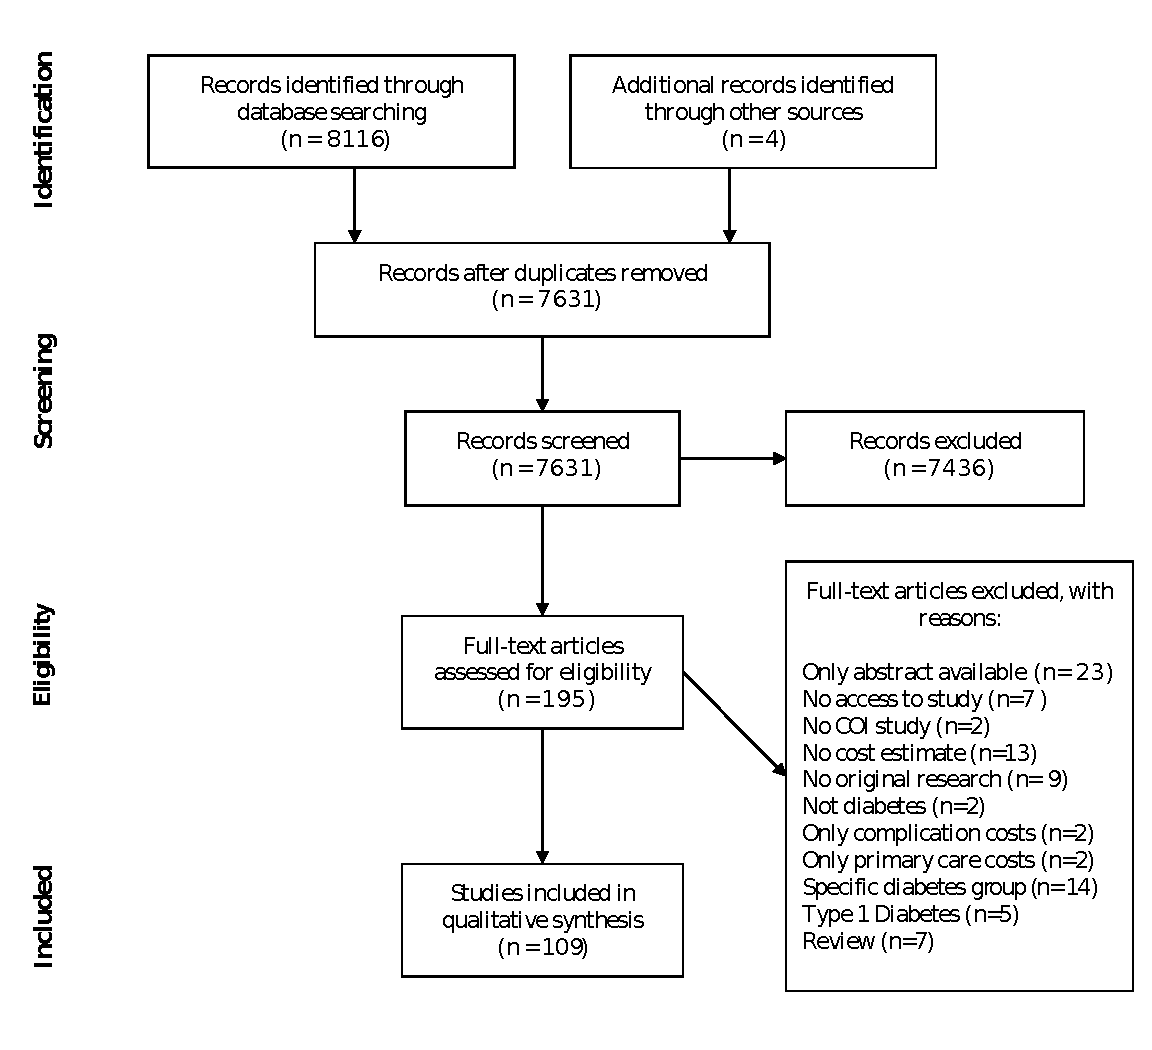
\includegraphics[width=0.9\linewidth]{Review/Figures/Fig1.eps}
\end{figure}

We present the \ac{COI} study results in per capita values to facilitate comparability across countries. For studies presenting overall population level estimates rather than per capita costs information, we calculated those costs, whenever possible, using the diabetes prevalence mentioned in the respective study. If no total cost estimate was presented but information on direct and indirect costs was available, then direct and indirect costs were added up to produce a total cost estimate. We converted costs into \ac{PPP} adjusted estimates, also called international dollars and henceforth denoted with the \$ sign, in order to further increase comparability. Since some studies did not present the data in the country's local currency but in USA\$ or some other major currency, we used the exchange rate given in the article to convert the estimates back into the local currency. If no exchange rate was provided in the study itself, the average exchange rate (midpoint exchange rate according to OANDA historical exchange rates---[\url{http://www.oanda.com/currency/historical-rates/}]) for the reported year. The \ac{PPP} adjusted estimates for the year 2011 were then calculated using the Campbell and Cochrane Economics Methods Group Evidence for Policy and Practice Information and Coordination Centre (CCEMG-EEPPI Centre) cost converter \parencite{Shemilt2010}. For all additional analyses carried out in the following sections only studies for which a mean cost estimate was presented or could be calculated, were included. Further, in the case of a study presenting estimates for more than 1 year, only the estimate for the most recent year was used for the analysis. For studies presenting both incremental and total cost estimates, only the incremental cost estimate was taken into account.

Studies were further classified into two groups according to the level of economic development of the investigated country---(1) high-income and (2) \acp{LMIC} (\acp{LMIC})---according to the historical World Bank income group classification of the respective country in the year that data collection for the respective study had taken place \parencite{WorldBank}. Where necessary due to space constraints we used abbreviations for country names, as detailed in Table \ref{tab:review_countries} in the appendix.

In order to explore the factors involved in the variation of direct costs reported in \ac{COI} studies, we first plotted the direct per capita costs in relation to the \ac{GDP} per capita of the respective country and provided an estimate of the relationship using linear regression. We then conducted an exploratory regression analysis, with the annual direct cost per patient as the dependent variable to investigate what other factors might explain the variation in direct cost estimates. The set of independent variables comprised (1) the estimation approach in each study, (2) the year of data used, (3) \ac{GDP} per capita of the studied country in international dollars, (4) an indicator of whether the study was conducted in the USA, (5) an indicator of whether the study was deemed to be nationally representative, and (6) a variable indicating whether the study had explicitly taken diabetes-related complications into account. The year of the data used was considered because the development of social security systems and treatment methods may affect how the direct costs evolve over time. We categorized this variable into groups: studies using data from before 1995, 1995 to 1999, 2000 to 2004, 2005--2009 and 2010--2004.  The dummy variable for studies on the USA was included to account for the generally higher healthcare expenditures in the USA compared which other \acp{HIC} with similar per capita income levels \parencite{Laugesen2011}. Accounting for national representativeness should cancel out any effects that might be driven by those studies that estimate costs for sub-national, regional- or city-level population samples. Including an estimator for diabetes complications should account for the possible underestimation of diabetes costs in studies excluding complications. We exclude country estimates extracted from multi-country studies in our preferred specification, as their inclusion would lead to an over-statement of the cost effect of the estimation method employed in the given multi-country study. 

\section{Results}
Due to the differences in methodologies, we first present the findings on the identified \ac{COI} studies and subsequently turn to studies on labour market outcomes.

\subsection{Cost-of-illness studies on type 2 diabetes}

\subsubsection{Number of studies}
We identified a total of 86 relevant \ac{COI} studies (see Table \ref{tab:COI_charactersitics} in the appendix for a detailed description of the included studies), of which 62 focused on \acp{HIC}, 23 on \acp{LMIC}, and one multi-country study covered both \acp{HIC} and \acp{LMIC}. Studies in \acp{LMIC} increased over time, with the majority of the \ac{LMIC} studies being published between 2007 and 2014. Six of the selected studies were multi-country studies, of which two \parencite{Kirigia2009,Smith-Spangler2012} did not provide detailed cost estimates for every country in the study and one did not provide a year for the estimated costs, so that we could not calculate estimates in international dollars \parencite{Boutayeb2014}. Therefore, we could not include these particular studies in our country-specific analysis.

\subsubsection{Regional distribution}
In terms of geographic regions, most studies were carried out on countries in Latin America and the Caribbean (n=38) and Europe (n=37), followed by the USA and Canada (n=26), East Asia and Pacific (n=11), the Middle East and North Africa (n=5), South Asia (n=4), Sub-Saharan Africa (n=4) and Australia (n=1). The number of countries studied is higher than the number of articles reviewed due to four multi-country studies \parencite{Boutayeb2014,Barcelo2003,Jonsson2002b,Abdulkadri2009b}, estimating costs for multiple countries. The USA were the most studied country (n=19), followed by Canada (n=7) and Germany (n=5). Mexico (n=6) and China (n=4) were the most frequently studied \acp{LMIC}.

\subsubsection{Data sources}
Especially in \acp{LMIC}, self-administered surveys represented a popular method to retrieve data on the cost of diabetes. These were mostly limited regionally, i.e. to a city or hospital, and usually only representative of these regional diabetes populations but not of a national population. In \acp{HIC}, databases of insurance and healthcare providers were the main source of information in most studies. These data tended to be representative either at a national or at some sub-national level. As a result, the size of the samples in \acp{HIC} was mostly between 1,000 and several million. By contrast, studies in low- and lower-middle-income countries were generally characterized by smaller sample sizes, ranging from 35 \parencite{Suleiman2006} to about 2,433 \parencite{Yang2012} in the studies reviewed here.

\subsubsection{Variation in costing approaches}
As discussed in more detail in Text Box 1, a range of costing approaches can be found in the \ac{COI} literature. Figure \ref{fig:review_COI_number} shows that the most common costing method for the direct costs of diabetes in \acp{HIC} was the sum-all medical approach for people with diabetes without using control groups \parencite{Kirigia2009,Boutayeb2014,Barcelo2003,Jonsson2002b,Ohinmaa2004,Lau2011a,Pohar2007,Gonzalez2009b,Horak2009,Martin2007b,Nolan2006c,Lucioni2003,Morsanutto2006b,Nakamura2008,Arredondo2004,Arredondo2007,Arredondo2005a,Arredondo2011b,Redekop2002b,Bjegovic2007b,Oliva2004a,Ringborg2008a,Chi2011a,Zhou2005a,Condliffe2014,Brandle2003d,Peele2002a,Lee2006,Maciejewski2004}. 

The disease-attributable costing approach \parencite{Suleiman2006,Abdulkadri2009b,Davis2006b,Simpson2003,RodriguezBolanos2010a,Solli2010a,Ballesta2006,Mata2002a,Lin2004,Dall2003a,Buescher2010,Tunceli2010c,Johnson2006d,Honkasalo2014,Bastida2002} and the attributable-fraction approach were also used widely, though mainly in the USA \parencite{AmericalDiabetesAssociation2008,Dawson2002b,Schmitt-Koopmann2004b,Dall2010,Bolin2009d,Honeycutt2009a,Lesniowska2014}. 

The incremental cost approach was applied primarily in studies on \acp{HIC} \parencite{Smith-Spangler2012,Yang2012,Tunceli2010c,Honeycutt2009a,Pohar2007a,Ricordeau2003,Koster2011c,Koster2006c,Koster2012,Esteghamati2009,Chodick2005a,Marchesini2011b,Bruno2012,Norlund2001a,Wirehn2008b,Birnbaum2003c,Durden2009b,Rodbard2010b,Oconnell2012,Trogdon2008a,Ramsey2002a,VanderLinden2009c}.  

For \acp{LMIC}, the survey approach was the most used \parencite{Wang2009b,Wang2009f,Chan2007a,Ramachandran2007d,Javanbakht2011b,Khowaja2007a,Biorac2009a,Elrayah-Eliadarous2010b,Chatterjee2011c,Al-Maskari2010c,Druss2001,Tharkar2010a,Wang2010c}.


\begin{figure}[p]
\caption{\label{fig:review_COI_number}Number of \acs*{COI} studies, by costing approach and income group.}%

\begin{minipage}{\linewidth}
\begin{center}
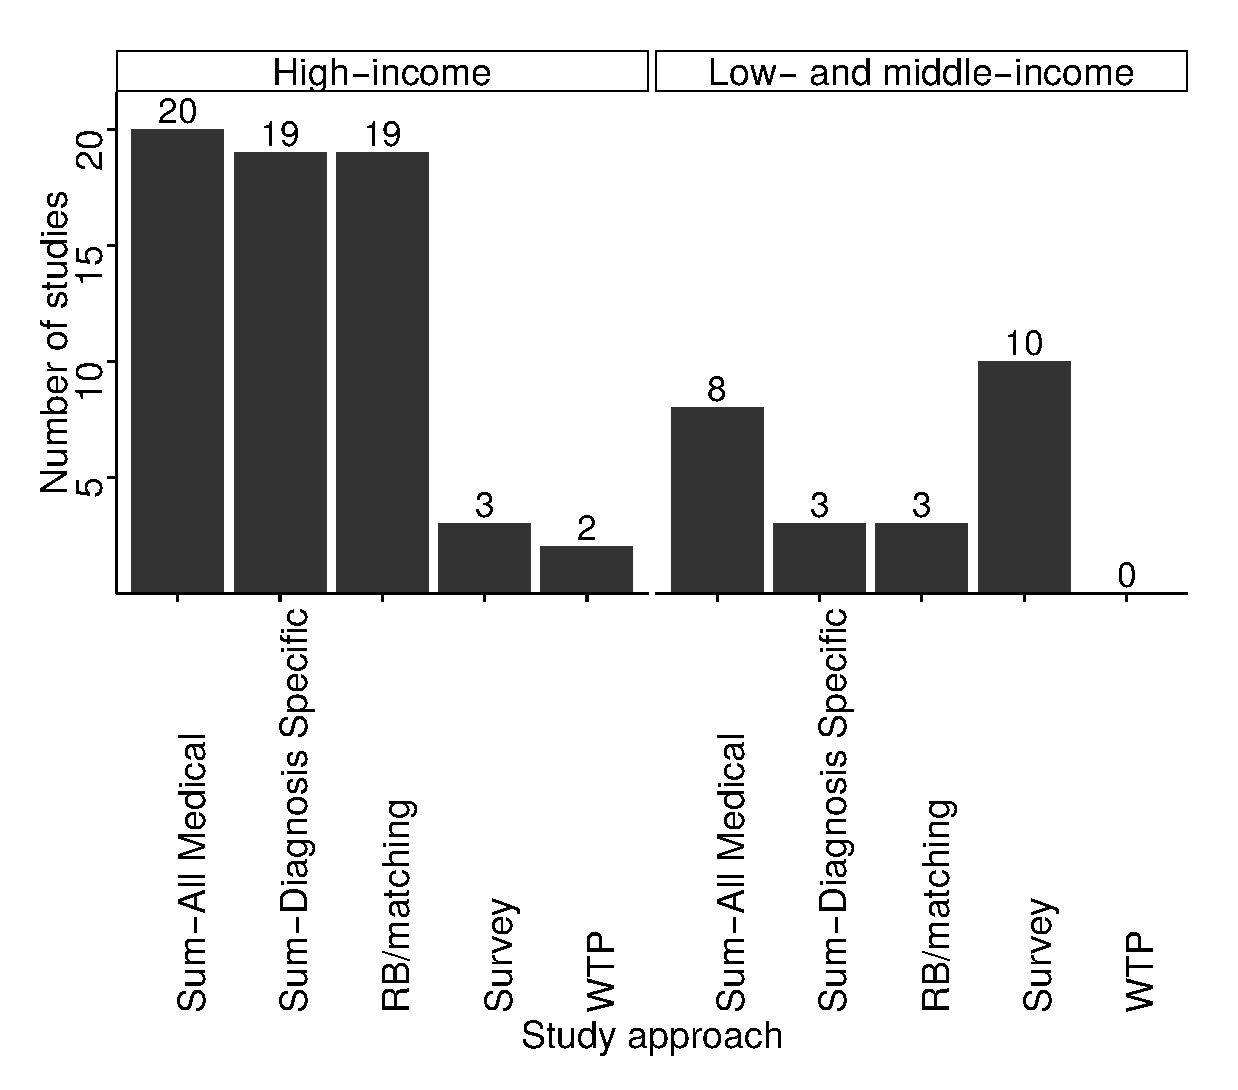
\includegraphics[width=0.8\linewidth]{Review/Figures/Fig2.eps}\\
\end{center}
\footnotesize \textit{Notes} For \acp{LMIC} no \ac{WTP} study is counted, because the only study \parencite{Tharkar2010a} presenting a \ac{WTP} estimate for a \ac{LMIC} used primarily a different approach to estimate costs, and the \ac{WTP} estimate was only presented additionally. Therefore this study was not counted under \ac{WTP} here. Two studies are counted twice as they give estimates for a sum-diagnosis specific and a RB/matching approach.
\end{minipage}
\end{figure}

By contrast, almost all indirect cost assessments followed the same methodology, i.e. the human capital approach. This approach considers all forgone labour earnings of a patient or caregiver that are attributable to diabetes. A minority of three studies \parencite{Tharkar2010a,Chang2010b,Gyldmark2001}, estimated the indirect costs using the \ac{WTP} approach, which tries to measure how much individuals would be willing to pay to reduce the risk of an illness \parencite{Segel2006}, here diabetes (or certain complications associated with it). One of the studies included \ac{WTP} estimates in addition to the direct and indirect costs measured by the human capital approach \parencite{Tharkar2010a} but did not include the \ac{WTP} estimate in the overall cost estimate, while the other two studies estimated exclusively the \ac{WTP} \parencite{Chang2010b,Gyldmark2001}.


\subsubsection{Study perspective}
Studies also varied in their perspective, again compromising direct comparability of the cost estimates across studies. Overall, most studies either took a societal (n=32) or healthcare system perspective (n=48). The former generally takes into account the direct and indirect monetary costs that arise to society, including costs to the healthcare system, costs due to lost productivity and sometimes \ac{OOP} costs \parencite{Segel2006}. The latter was especially common in \acp{HIC} where many studies assessed the cost of diabetes to private or public health insurances. In \acp{LMIC}, studies often took the patient perspective (n=5), estimating \ac{OOP} expenditures and in some cases productivity losses, directly arising to the diabetes patient.

%Textbox
\fbox{\parbox[c]{\linewidth}{\textbf{Text box 1 \ac{COI} methodologies}
\begin{footnotesize}

Methodologies for \ac{COI} studies can broadly be categorized into two main categories:(1) estimating the total disease costs and (2) estimating the incremental costs \parencite{Akobundu2006}. Studies can then be divided further according to the specific approach used for estimation. Our categorization builds on that by \textcite{Akobundu2006} in their review of \ac{COI} methodologies.

\begin{enumerate}

\item Total disease costs
\begin{enumerate}
\item Sum-All Medical: captures all medical expenditures of a person diagnosed with diabetes, irrespective of the relation of the expenditures with diabetes.

\item Sum-Diagnosis Specific: includes the costs that are related to diabetes. This can be done by using a disease-attributable costing approach, using administrative claims databases to identify the cost of diabetes by respective \ac{ICD} codes that link the expenditures to a primary or secondary diagnosis of diabetes as the reason for the healthcare utilization. Alternatively, a similar technique used at the population level is the attributable-fraction approach, where the relative contribution of, e.g., diabetes, to the risk of developing another disease (e.g. renopathy or cardiovascular disease) is used to determine how much of the costs of this disease can be attributed to diabetes.

\item Survey approach: while not specifically mentioned by \textcite{Akobundu2006}, for this review we create a separate category capturing studies using surveys of people with diabetes. This category differs from the two approaches a) and b) above in that estimations rely solely on the individual, reported experience of people with diabetes, without use of any diagnostic data at an aggregate level. The survey approach was also used as a separate category in the earlier review on diabetes \ac{COI} studies by \textcite{Ettaro2004}.
\end{enumerate}

\item Incremental disease costs

There are two main approaches for the estimation of incremental medical costs:
\begin{enumerate}

\item Regression approach: a statistical technique which can account for observable differences between the group with diabetes and the control group (i.e. those without diabetes) to find---ideally---the independent effect of diabetes on healthcare costs. The differences typically accounted for are age, region and gender.

\item Matching approach: uses a control group to directly compare those with diabetes to those without diabetes after matching each person of the 'treatment' group to a 'similar' person of the control group, using various categories like age, region and gender to---again---find the independent effect of diabetes on healthcare cost \parencite{Akobundu2006}.
\end{enumerate}
\end{enumerate}

All of the above approaches can be used in prevalence or an incidence based study. In the former case the costs of diabetes are estimated for a certain point in time, typically one year, while the latter approach estimates costs over a person's lifetime or several years, always starting with the point at which the disease is diagnosed. Both approaches may also be combined in studies estimating the future cost burden of type 2 diabetes by first taking a prevalence approach to calculate current costs and then using predictions about future diabetes incidence rates to arrive at an estimate of diabetes costs at a certain point in the future.\end{footnotesize}
}}

\subsubsection{Costing components}
Of the 75 studies that reported the cost components they used to estimate direct costs, 72 took into account outpatient hospital visits, 70 inpatient hospital visits, 63 physician visits, 58 drug costs, 51 laboratory costs for diagnostic tests and check-ups, 37 equipment costs and 21 non-medical and transportation costs. A total of 46 studies had at least included the costs of hospital, outpatient and physician visits as well as drugs (see Table \ref{tab:costing_components} for a detailed description of cost components used in each study).

\subsubsection{Cost estimates of diabetes using a prevalence approach}

Two basic epidemiological approaches exist for the estimation of \ac{COI}, and they  are not directly comparable. The incidence approach follows people with diabetes, usually starting with their diagnosis at a common base year, estimating yearly costs for a sample of people at the same disease stage, finally giving an estimate of diabetes costs over a certain time period, such as from diagnosis to death or over a distinct period of, for example, 10 years. This approach can also document how costs of diabetes change and develop over the progression of the disease \parencite{Larg2011}. By contrast, the prevalence approach estimates the costs of diabetes for a cross-section of people with diabetes at a certain point in time, normally a year, who are at different stages of the disease. It is most suitable for assessing the total economic burden of diabetes at a certain point in time. Due to this difference in time periods and the data used, the estimates of prevalence-based studies are not directly comparable with those of incidence-based studies. Hence, we present the cost estimates, starting with the prevalence approach.

Table \ref{tab:review_regression} shows the range of direct cost estimates by estimation approach and income status.  As can be observed, direct cost estimates varied widely, both between and within the different estimation approaches. Cost estimates for direct costs, irrespective of the costing method applied and the cost components included, ranged from \$242 for Mexico \parencite{Arredondo2005a} in 2010 to \$11,917 for the USA \parencite{Condliffe2014} in 2007. Also, studies from \acp{LMIC} generally indicated smaller direct costs than studies from \acp{HIC}.

For indirect costs, studies using the human capital approach estimated costs ranging from \$45 for Pakistan \parencite{Khowaja2007a} in 2006 to \$16,914 for the Bahamas \parencite{Barcelo2003} in 2000. Three studies estimated indirect costs by using the \ac{WTP} approach and found costs ranging from \$191 in a study on the \ac{WTP} for a health insurance for type 2 diabetes in Denmark in 1993 \parencite{Gyldmark2001}, a \ac{WTP} \$4,004 per year for a cure of type 2 diabetes \parencite{Chang2010b} in Taiwan  and an annual payment of \$4,737 to halt disease progression/prevent future complications of diabetes in India \parencite{Tharkar2010a}. 

Societal costs of type 2 diabetes, which are estimated by studies combining direct and indirect costs, ranged from \$544 in a study on the economic costs of diabetes in Iran \parencite{Esteghamati2009} in 2001 to \$18,224 for the Bahamas \parencite{Barcelo2003} in 2000. 

\begin{table}[p]
\begin{center}

\begin{threeparttable}
\begin{tabularx}{\linewidth}{X X X X X X X X X}
\caption{\label{tab:review_direct_costs_summary}Summary of direct costs by estimation approach and income status in international dollars \$ (2011) for prevalence-based studies.}\\
\toprule
& \multicolumn{4}{l}{High-income countries} & \multicolumn{4}{l}{Low- and middle-income countries} \\ \midrule
 & Sum-all medical costs & Sum-diagnosis specific & RB / matching & own survey & Sum-all medical costs & Sum-diagnosis specific & RB / matching & own survey \\ \midrule \endfirsthead
\caption[]{Summary of direct costs by estimation approach and income status in international dollars \$ (2011) for prevalence-based studies.}\\
 \toprule
 & \multicolumn{4}{l}{High-income countries} & \multicolumn{4}{l}{Low- and middle-income countries} \\ \midrule
  & Sum-all medical costs & Sum-diagnosis specific & RB / matching & own survey & Sum-all medical costs & Sum-diagnosis specific & RB / matching & own survey \\ \midrule \endhead
Min & 1117 & 907 & 264 & 1495 & 242 & 662 & 443 & 456 \\
Max & 11917 & 9346 & 8306 & 5585 & 4129 & 4672 & 1136 & 3401 \\
N & 25\textsuperscript{a} & 19\textsuperscript{a} & 18 & 3 & 27\textsuperscript{a} & 5\textsuperscript{a} & 2 & 10\\
 \bottomrule
\end{tabularx}
\begin{tablenotes}
\item \footnotesize \textit{Notes} \textsuperscript{a} Includes country estimates from multi-country studies; RB Regression based
\end{tablenotes}
\end{threeparttable}
\end{center}
\end{table}


In order to improve the cross-country comparability of the costs of diabetes we plotted the results from studies providing a direct per capita cost estimate against the \ac{GDP} per capita estimate of the respective country (we limited this comparison to studies using samples representative of their entire population). Figure \ref{fig:review_GDPtocost_ratio} confirms the expectation that costs do increase with economic wealth: \ac{GDP} per capita explains about one-third of the variation in cost estimates (see r2 in Figure \ref{fig:review_GDPtocost_ratio}). Also, studies on the USA seem to estimate costs consistently higher than would be expected on the basis of its \ac{GDP} per capita. 

The USA, however, spend consistently more than what would be expected on the basis of its \ac{GDP} per capita. Again, the wide variation in estimated costs for many countries underscores the point that the studies need to be contextualized and may not be directly comparable per se. On the whole---though by no means always---the matching and regression as well as the sum-diagnosis specific approaches appear to produce lower cost estimates than especially the total cost results, particularly so for \acp{HIC}. In an inevitably crude attempt to quantitatively explore the driving factors behind the heterogeneity in cost estimates, we estimated a simple linear regression model with per capita direct costs as the dependent variable; explanatory variables included \ac{GDP} per capita, the estimation approach employed by the study, the number of included cost components, a dummy for studies carried out in the USA, the year of data collection, the representativeness of the study and if the study included diabetes complications as explanatory variables. The results, displayed in Table \ref{tab:review_regression}, show a strong relationship between \ac{GDP} per capita and expenditures for diabetes, with every additional international dollar in per capita \ac{GDP} translating into an average increase in direct diabetes expenditures of about \$0.04. The estimation approach is not found to matter significantly, nor is the year of study. Estimates from USA studies put the costs at over \$3,000 higher (on average) than studies from other countries, indicating that costs in the USA may indeed be unusually high. The number of costing components and the inclusion of complications likely also explain some of the variance in estimates, although they are just below and above the 10\% significance level, respectively. Overall, the included independent variables explain about 56\% of the variation in direct cost estimates. In a sensitivity analysis, we included the results from multi-country
studies providing country estimates in the regression analysis. The
only major difference to the presented analysis is that the inclusion of
complications as well as the number of included cost components
were now significant at the 1\% and 5\% significance level, respectively.
The effect size and significance of the other estimates did not change
considerably.


\begin{figure}[p]
\caption{\label{fig:review_GDPtocost_ratio}\acs*{GDP} to direct costs ratio by estimation approach.}%
\begin{minipage}{\linewidth}
\begin{center}
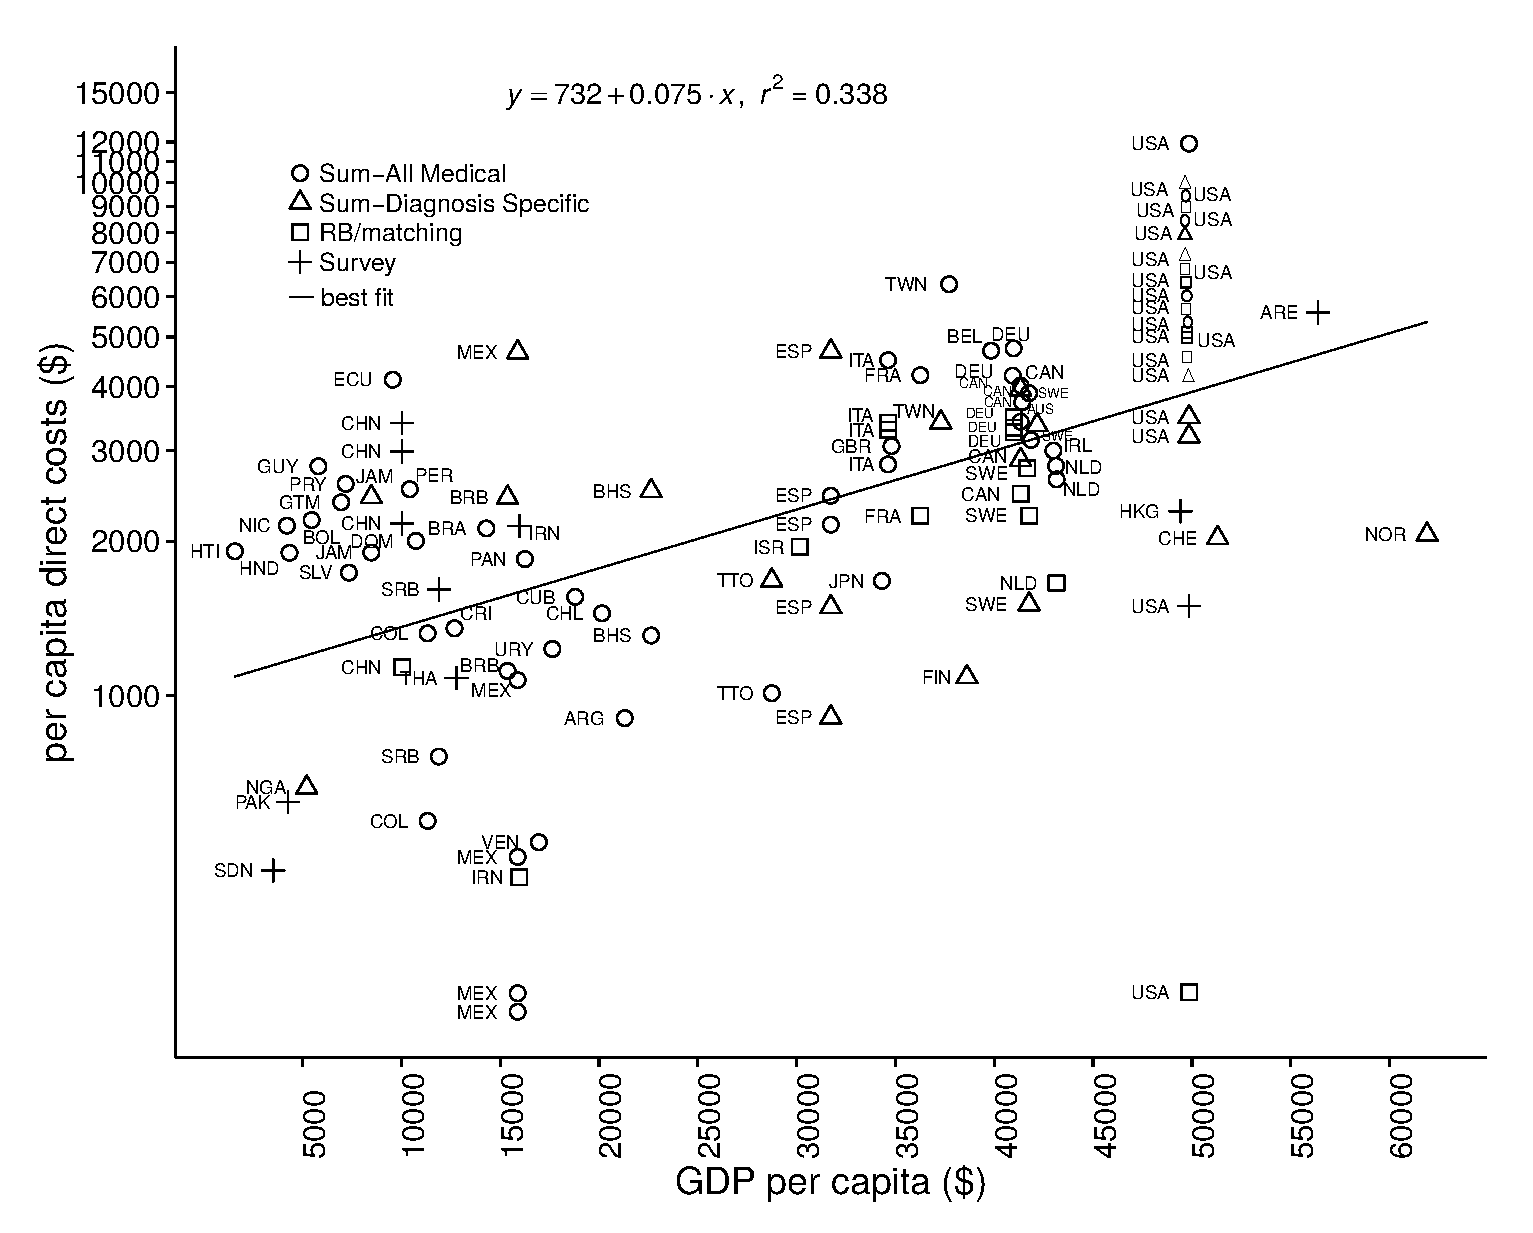
\includegraphics[width=1\linewidth]{Review/Figures/Fig3.eps}\\
\end{center}
\footnotesize
\textit{Notes}  The line depicts the best fit based on the linear regression of direct costs on \ac{GDP} per capita in international dollars.
\end{minipage}
\end{figure}





\begin{table}[p]
\caption{\label{tab:review_regression}Relationship between direct costs and study characteristics (robust linear regression).}
\begin{center}
\begin{adjustbox}{max width=\linewidth}
\begin{threeparttable}
{
\def\sym#1{\ifmmode^{#1}\else\(^{#1}\)\fi}
\begin{tabular}{l*{2}{SS}}
\toprule
                 &\multicolumn{1}{c}{Estimate} &\multicolumn{1}{c}{Std. Error} \\ \midrule
                Constant & 2133 & 1773.922 \\
                GDP per capita (\$) & .045\sym{**} & 0.017 \\
                Estimation Approach &  &  \\
                \hspace*{10mm}Sum-All medical (Ref.) & &  \\
                \hspace*{10mm}Sum-Diagnosis Specific & -413.880 &  528.766 \\
                \hspace*{10mm}RB/matching & -719.868 &  526.896 \\
                \hspace*{10mm}Survey & -689.806 & 671.020 \\
                At least four costing components & 702.966\sym{*} & 403.968 \\
                USA study & 3111.067\sym{***} & 533.534 \\
                Year of study &  &  \\
                \hspace*{10mm}\textless1995 (Ref.) &  &  \\
                \hspace*{10mm}1995-1999 & -1744.799 & 1632.498 \\
                \hspace*{10mm}2000-2004 & -816.647 & 1586.966 \\
                \hspace*{10mm}2005-2009 & -1021.685 & 1592.595 \\
                \hspace*{10mm}2010-2014 & -2744.739 & 1839.689 \\
                Study representative & -598.670 & 409.070 \\
                Complications & 666.803 & 414.727 \\
\midrule
                R-squared adj. & .559 &  \\
                N & 70 &  \\ 
 \bottomrule
\end{tabular}
\begin{tablenotes}
\item \footnotesize \textit{Notes} Standard errors in parenthesis. Ref. reference category.
\sym{*} \(p<0.10\), \sym{**} \(p<0.05\), \sym{***} \(p<0.01\).
\end{tablenotes}
}
\end{threeparttable}
\end{adjustbox}
\end{center}
\end{table}

The sensitivity of the cost results to the estimation approach was also examined by two studies that investigated the effect of different estimation techniques in diabetes \ac{COI} studies. \textcite{Honeycutt2009a} compared the use of a regression-based and an attributable-fraction approach and found that the cost estimate of the former exceeded the latter by 43\%. \textcite{Tunceli2010c} compared the matching and the diabetes (disease)-attributable costs approach and found a 14--29\% higher cost estimate using matching, depending on the assumptions used. Both studies concluded that an incremental cost approach results in a higher, and likely more exact, estimate of the direct costs of diabetes than disease-attributable approaches. The authors attributed this to the fact that a regression or matching approach can assign costs to diabetes that cannot be linked to diabetes otherwise. Those approaches are therefore in a position to account for all costs of co-morbidities caused by diabetes, while this is not automatically the case with the other approaches.

\subsubsection{Direct and indirect costs of diabetes}

Comparing the relative importance of direct and indirect costs across countries may provide some information regarding the underlying drivers of costs due to diabetes in different countries. For instance, a higher ratio of direct to indirect costs may indicate that the higher direct expenditures have led to better treatment and less complications and thereby have reduced the productivity losses due to diabetes. We therefore plotted direct against indirect costs from studies that provided both estimates and drew a 45\degree line depicting the equal share of direct and indirect costs (see Figure \ref{fig:review_direct_indirect}). Studies above the line found higher direct costs compared to indirect costs and studies below the line found higher indirect costs compared to direct costs.

Most studies found a larger share for direct costs in comparison with indirect costs. This is especially true for \acp{HIC}, where only a study on Sweden \parencite{Bolin2009d} found a larger share for indirect costs. For \acp{LMIC}, a study on Colombia \parencite{Gonzalez2009b} found considerably higher indirect costs, as did the multi-country study of \textcite{Barcelo2003} and a study on various countries in the African region \parencite{Kirigia2009}, which both found higher indirect costs for almost every country in the study and also on average for the entire region, represented as the mean overall study estimate in Figure \ref{fig:review_direct_indirect}.  Both studies used similar approaches to estimate costs, and indirect cost estimates were likely so high because evidence from only a few countries within the region was used as a basis for estimating indirect costs for every other country in the respective study. Further, the studies took the countries' per capita gross national product as a proxy for earnings, which might have led to an over-estimation of the indirect costs \parencite{Kirigia2009}. 

Overall, no clear pattern emerges that would indicate that in \acp{LMIC} indirect costs would be higher than direct costs due to their less extensive healthcare systems, or that \acp{HIC} would be able to prevent indirect costs as a result of their higher healthcare spending. For instance, while some studies indicated that \acp{MIC} such as Colombia and Mexico have higher indirect costs, studies on China, Pakistan and, again, Mexico showed the opposite. Difficulties in measuring costs could be one of the main reasons for the heterogeneity in results even for the same country and may make a comparison of direct and indirect costs difficult. In particular in \acp{LMIC} countries, direct healthcare expenditures may be low due to limited availability and access to healthcare so that direct costs would be higher if more treatment options were available. Indirect costs may also be incorrectly measured, for example the use of the human capital approach---which estimates the potential instead of of the actual lost production, e.g. assuming that a sick individual cannot be replaced by a previously unemployed individual, even though in reality production losses may only be temporary until the employer has found a replacement---may lead to an overestimation of the losses in productivity \parencite{Segel2006}. 

\begin{figure}[p]
\caption{\label{fig:review_direct_indirect}Direct and indirect cost relation in studies estimating total costs of type 2 diabetes.}%
\begin{minipage}{\linewidth}
\begin{center}
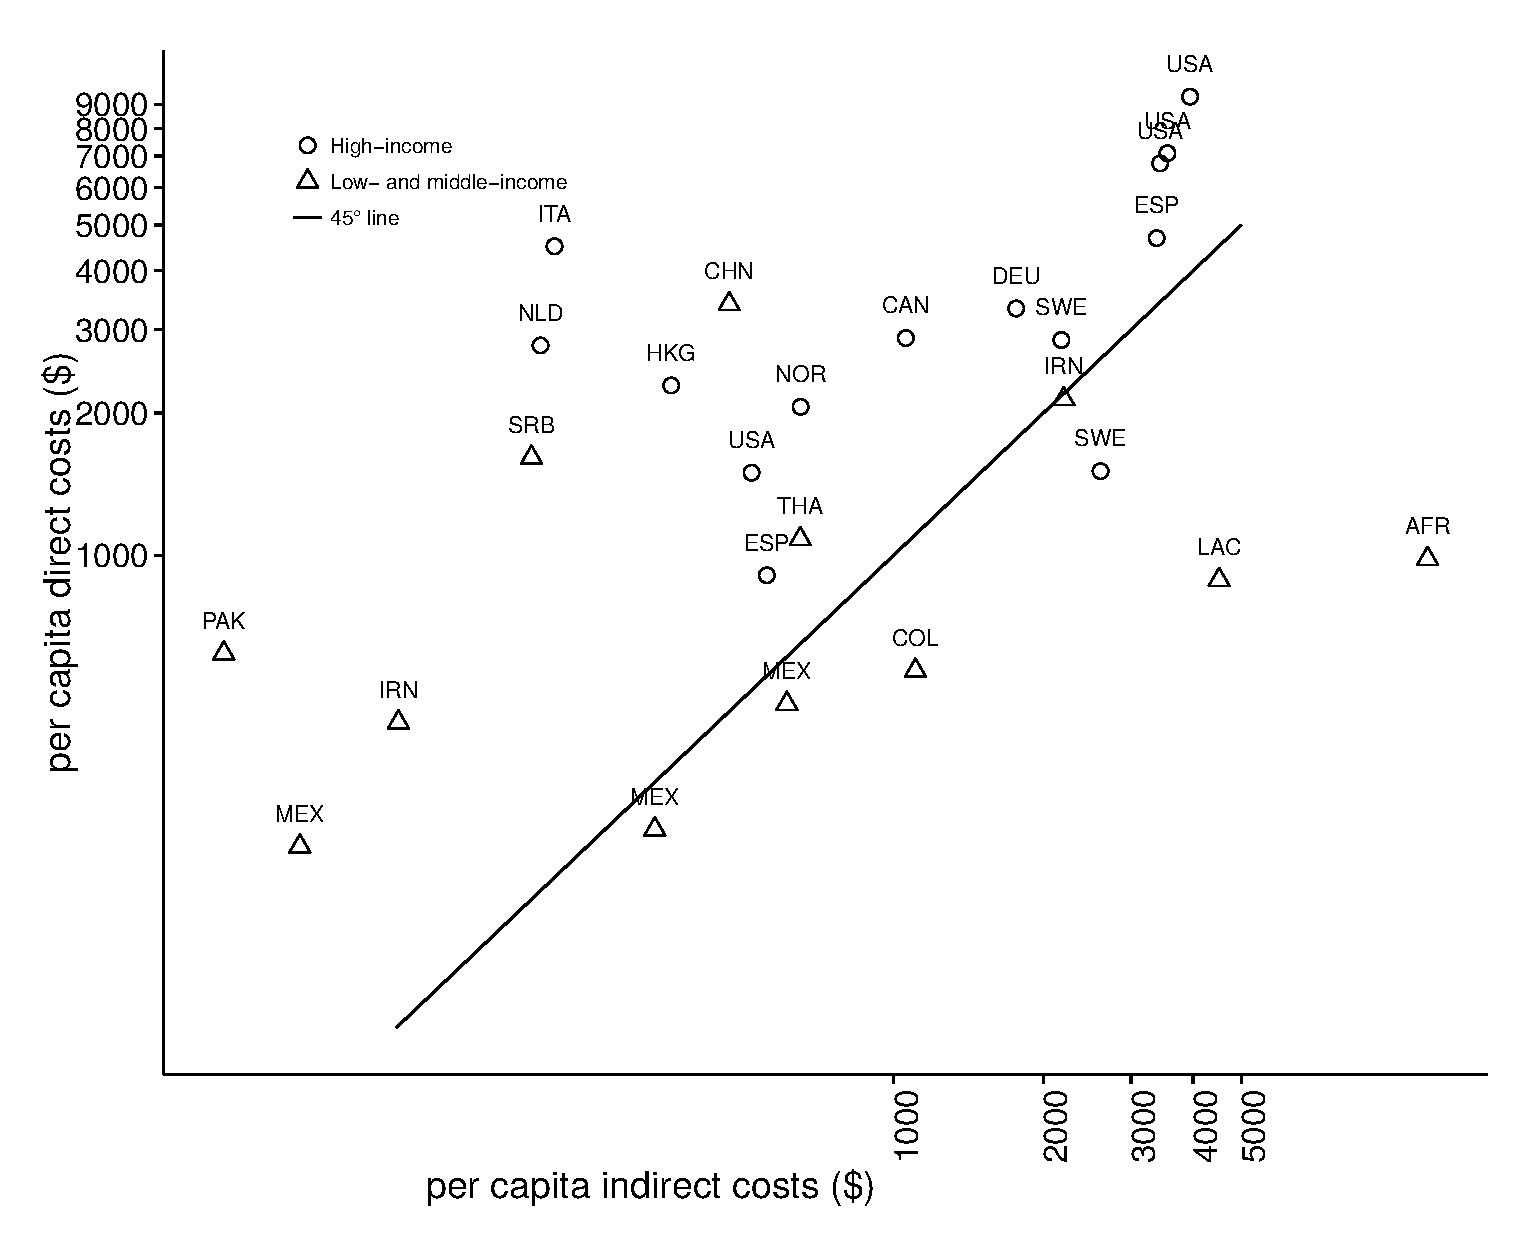
\includegraphics[width=1\linewidth]{Review/Figures/Fig4.eps}\\
\end{center}
\footnotesize
\textit{Notes} The 45\degree line depicts the points where direct and indirect costs would be equal. Above the line direct costs are higher than indirect costs and vice versa. For better visibility both coordinate axes are expressed in log scale
\end{minipage}
\end{figure}

\subsubsection{Studies using the incidence approach}
The four studies that used an incidence approach (see Table \ref{tab:review_incidence}) estimated the cost of diabetes either over a person's lifetime \parencite{Gonzalez2009b,Birnbaum2003c} or over a certain period after diagnosis \textcite{Johnson2006d,Martin2007b}. \textcite{Gonzalez2009b} modelled the lifetime (direct and indirect) costs of a typical diabetes patient in Colombia, arriving at a mean cost estimate of \$54,000. The second study providing lifetime estimates by \textcite{Birnbaum2003c}, estimated incremental lifetime healthcare costs for USA females with diabetes of \$283,000.

Two studies followed patients over a limited time period and found different patterns in the development of type 2 diabetes-attributable healthcare costs. In Germany costs increased from  \$1634 in the first year after diagnosis to \$4881 in the seventh year \parencite{Martin2007b}. In Canada, \textcite{Johnson2006d} found the highest costs in the year of diagnosis with \$7635, up from \$2755 the year prior to diagnosis. In the year after diagnosis costs decreased to \$4273 and then only increased slightly to \$4618 in year ten. In Germany and Canada, costs related to complications or hospital visits were the most important components and in Germany increased steadily over time. In Canada costs related to prescriptions increased the most.

\clearpage
\begin{landscape}

\begin{tabularx}{\linewidth}{m m m b m b}
\caption{Incidence studies on the costs of diabetes}\label{tab:review_incidence}\\
\toprule
Ref. &  Country & Time horizon & Population & Approach & \multicolumn{1}{c}{Results} \\
 \midrule \endfirsthead
\caption[]{Incidence studies on the costs of diabetes}\\
\toprule
Ref. &  Country & Time horizon & Population & Approach & \multicolumn{1}{c}{Results} \\ \midrule \endhead
\textcite{Johnson2006d} &  Canada & 1992--2001 & Incidence T2D patients from Saskatchewan Health's administrative database in Canada & Sum-all medical & Highest  total healthcare costs at year of diagnosis with CAN\$7343 (\$7635), then increased from a low of CAN\$3880 (\$4034) 3 years after diagnosis to CAN\$4441   10 years thereafter (\$4618). \\
	\textcite{Gonzalez2009b} & Colombia & 32 years & Hypothetical average Columbian T2D patient & Sum-all medical & Total lifetime costs (32 year  period) of average diabetes patient, including direct and indirect costs,  57.565 million Colombian pesos (\$54,351). \\
\textcite{Martin2007b} & Germany & 1995--2003 & Newly  diagnosed T2D patients from randomly drawn practices across Germany & Sum-all medical & EUR 1,288   (\$1635) for the first treatment year after diabetes diagnosis and increased   to EUR 3845 (\$4880) in the seventh year. \\
\textcite{Birnbaum2003c} & United  States & 1997--1998 & Women employed by nationwide operating company and hypothetical women above age 64 receiving Medicare & RB / matching & \$282973 incremental lifetime direct healthcare costs, using incidence-based, steady-state methodology. \\ \bottomrule
\multicolumn{6}{l}{\footnotesize \textit{T2D} type 2 diabetes}
\end{tabularx}


\end{landscape}



\subsubsection{Country level costs prediction studies}
Four studies projected costs of diabetes over a certain period of time \parencite{Ohinmaa2004,Lau2011a,Davis2006b,Wang2009f}, making assumptions about the future development of diabetes prevalence and population ageing (see Table \ref{tab:review_prediction}). For Canada, a 1.7-fold increase from 2000 to 2016 \parencite{Ohinmaa2004} and a 2.4-fold increase from 2008 to 2035 in diabetes healthcare costs was estimated \parencite{Lau2011a}. Taking a health care system perspective, both studies found that the estimated increase would be mostly driven by an ageing population. For Australia, \textcite{Davis2006b} estimated a 2.5- to 3.4-fold increase in diabetes attributable healthcare costs from 2000 to 2051, depending on the underlying assumptions about population ageing and diabetes prevalence rates. For China, \textcite{Wang2009f} extrapolated total costs of diabetes from the year 2007 to 2030, estimating the costs of diabetes to increase 1.8-fold, solely accounting for the expected increase in prevalence.

\begin{table}[p]
\begin{tabularx}{\linewidth}{m m m m m b}
\caption{Country level costs prediction studies}\label{tab:review_prediction}\\
\toprule
Ref. & Country & Population   & Approach & Time  horizon & \multicolumn{1}{c}{Results}                                                                                                                                            \\ \midrule
\textcite{Davis2006b}  & Australia & Australian   population                       & Sum diagnosis  Specific & 2000--2051                                                              & If age and sex specific prevalence remains unchanged a 2.5-fold increase; if age and sex specific prevalence allowed to change as well a 3.4-fold increase. \\
\textcite{Ohinmaa2004}  & Canada    & Canadian   population                         & Sum-all   medical costs  & 2000--2016                                                              & 1.7-fold increase.                                                                                                                                          \\
\textcite{Lau2011a}  & Canada    & Four   Alberta Health and Wellness databases  & Sum-all  medical costs  & 2008--2035                                                              & 2.4-fold increase.                                                                                                                                          \\
\textcite{Wang2009f}  & China     & In   patients and outpatients in 20 hospitals & Own   survey             & 2007 and  2030 (projection) & Increase from \$73 billion in 2007 to \$132 billion in 2030 (1.8 fold increase).                                       \\ \bottomrule
\end{tabularx}
\end{table}

\subsection{The impact of diabetes on employment probabilities and productivity}
Besides studies that determined the cost of diabetes by costing related expenditures, another body of research has investigated---using econometric techniques---the impact of diabetes on 'productivity', a term used here to comprise outcomes including employment probabilities and lost work days and income or earnings. A recent study systematically reviewed evidence on the impact of diabetes on the ability to work, focusing on studies assessing the impact of diabetes on early retirement, lost work hours, absenteeism and presenteeism \parencite{Breton2013}. We focused particularly on studies exploring the impact of diabetes on employment probabilities and earnings---both issues that were not covered in the mentioned review---and we took a more detailed look at the empirical challenges posed by the issue of endogeneity (see page \pageref{sec:appendix_endogeneity} in the Appendix for a more detailed discussion of endogeneity).

Tables \ref{tab:rev_Diab_employment} and \ref{tab:rev_Diab_productivity} synthesize the relevant information from the 23 identified studies on the effect of diabetes on employment and other labour market outcomes. Almost all studies were conducted on \acp{HIC}, mainly the USA (n=13) and European countries (n=4). Only one study focused on a \ac{LMIC} investigating the effect of diabetes on labour income in China.

\subsubsection{Employment probabilities}
Most studies examined the impact of diabetes on employment probability (n=17), applying a range of econometric techniques. These have evolved over time, and more recent studies took into account the possibility that diabetes might be endogenous: it is conceivable that especially personal traits such as motivation and drive could influence the propensity to develop type 2 diabetes as well as a persons' job market opportunities. Further, being employed or unemployed could also lead to changes in lifestyles, due to changes in income, stress or leisure time, that could themselves affect the chances of developing diabetes \parencite{Brown2005}. Of the studies that tried to account for this problem \parencite{Brown2005,Minor2011,Latif2009,Lin2011b,Zhang2009,Harris2009}, the majority used an \ac{IV} technique. This approach allows for the consistent estimation of the effect of diabetes on employment if a variable can be found that is causally related to diabetes without affecting the employment probabilities through any other unobserved pathway apart from its effect on diabetes (see Text Box 1). In the case of type 2 diabetes all studies used the family history of diabetes as an \ac{IV} to exploit the fact that the development of type 2 diabetes is much more likely for individuals whose biological parents have also had diabetes. It is argued that, while controlling for education, age and other observable demographic and socioeconomic factors (e.g. wealth, regional and ethnic differences and the number of children in the household), having a family member with diabetes should not affect the person's employment status or other labour market outcomes, while strongly predicting the onset of type 2 diabetes. 

\newpage
\begin{landscape}
\begin{tabularx}{\linewidth}{m m m m b b}
\caption{Studies estimating the relationship between diabetes and employment (2001 -- 2014)}\label{tab:rev_Diab_employment}\\
\toprule
Ref & Survey year & Country  & Age     & \multicolumn{2}{c}{Effect on employment} \\ \cmidrule(l){5-6}                                                                                                                                                                                                                                                                                                                                                                              &  &  &   & \multicolumn{1}{c}{Males} & \multicolumn{1}{c}{Females} \\ \midrule \endfirsthead
\caption[]{Studies estimating the relationship between diabetes and employment (2001 -- 2014)}\\
\toprule
Ref & Survey year & Country  & Age     & \multicolumn{2}{c}{Effect on employment} \\ \cmidrule(l){5-6}                                                                                                                                                                                                                                                                                                                                                                              &  &  &   & \multicolumn{1}{c}{Males} & \multicolumn{1}{c}{Females} \\ \midrule \endhead
\textcite{Harris2009} & 1999-2000      & Australia                                                                                 & \textgreater24              & Exogenous: 10.8 percentage points reduction to be in labour force; endogenous: 7.1 percentage points reduction and test indicates endogeneity.                                                                                                           & Exogenous: 10 percentage points to be in labour force; endogenous: Nine percentage points reduction and test indicates endogeneity                                    \\
\textcite{Zhang2009} & 2001, 2004-2005 & Australia                                                                                 & 18-64                       & 50-64: 11.5 percentage points less likely to be in labour force; 18-49: 3.9 percentage points less likely, all effects increase when other chronic diseases are present.                                                                                   & No significant effect for diabetes alone; significant negative effect if other chronic diseases are present.                                                             \\
\textcite{Latif2009} & 1998           & Canada                                                                                    & 15-64                       & Exogenous: 19 percentage points less likely to be employed; endogenous: not significant and positive and test indicates endogeneity.                                                                                                                       & Exogenous: 17 percentage points less likely to be employed, endogenous: not significant and positive and test indicates exogeneity.                                      \\
\textcite{Kraut2001a} & 1983-1990      & Canada                                                                                    & 18-64                       &\merge{With complications 2 times less likely to be in labour force; no significant effect on employment for those in labour force.\textsuperscript{a}} \\
\textcite{Norlund2001a}  & 1992-1993      & Sweden                                                                                    & \textgreater24              & \merge{14.2 percentage points higher retirement rate (22.9 compared to 8.7).\textsuperscript{a}} \\
\textcite{Alavinia2008a} & 2004           & Sweden, Denmark, Netherlands, Germany, Austria, Switzerland, France, Italy, Spain, Greece & 50-65                       & \merge{For whole dataset: no effect of diabetes on being unemployed, but increased odds ratio of 1.33 on being retired. No information on effects by country.\textsuperscript{a}} \\
\textcite{Lin2011b} & 2005           & Taiwan                                                                                    & 45-64                       & Exogenous: 9 percentage points less likely to be employed; endogenous: 19 percentage points less likely to be employed; test on whole sample indicates endogeneity.                                                                                        & Exogenous: 11 percentage points less likely to be employed, endogenous: not significant and negative.                                                                    \\
\textcite{Brown2005}  &                & USA                                                                             & \textgreater44              & Exogenous: 7.4 percentage points less likely to be employed; endogenous: 10.6 percentage points less likely but test indicates exogeneity.                                                                                                                 & Exogenous: 7.5 percentage points less likely to be employed; Endogenous: no significant effect found and test indicates endogeneity.                                     \\
\textcite{Minor2011}  & 2006           & USA                                                                             & \textgreater19 at diagnosis &                                                                                                                                                                                                                                                            & Exogenous: 25.2 percentage points less likely to be employed, endogenous: 45.1 percentage points less likely to be employed.                                             \\
\textcite{Vijan2004} & 1992-2000      & USA                                                                             & 51-61                       & \merge{More likely to be retired in 1992 (adjusted OR 1.3). Over 8 years follow up spent 0.14 incremental years in retirement.\textsuperscript{a}}\\
\textcite{Bastida2002} & 1996-1997      & USA                                                                             & \textgreater44              & 7.5 percentage points less likely to be employed.                                                                                                                                                                                                          & No significant effect on employment probabilities found.                                                                                                                       \\
\textcite{BrownIII2011} & 2008           & USA                                                                             & 35-64                       & Diabetes negatively related to employment (5 percentage points reduction); better diabetes management (\ac{HbA1c}) positively affects employment probabilities; \ac{HbA1c} lowering of 10\% increases employment probability by 0.44 percentage points.                  & No significant effect on employment probabilities found.                                                                                                                       \\
\textcite{Tunceli2005a} & 1992,1994      & USA                                                                             & 51-61                       & 9 percentage points less likely to work without complications controlled for, with complications controlled for 7.1 percentage points less likely.                                                                                                         & 5.9 percentage points less likely to work without complications controlled for, with complications controlled for 4.4 percentage points less likely but not significant. \\
\textcite{Tunceli2009a} & 1997-2005      & USA                                                                             & 20-44 and 45-64             & \merge{20-44: proportion with work limitations 3.1\% higher; 45-64: proportion not working is 8.1\% higher; the proportion work disabled is 3.4\% higher; proportion with work limitations is 5.7\% higher (all compared to similar age group without diabetes).\textsuperscript{a}}\\
\textcite{Valdmanis2001} & 1990-1995      & USA                                                                             &                             & \merge{Unemployment rate for persons with diabetes was 16\% compared with 3\% among matched comparison group.\textsuperscript{a}} \\
\textcite{Ng2001b} & 1989           & USA                                                                             & \textgreater29 at diagnosis & \merge{3.6\% less likely of being employed (exogenous), 12\% for those with complications.\textsuperscript{a}}                                                                                                                                                                                                                                                                                                                                              \\
\textcite{Minor2013} & 1979-2010      & USA                                                                             & \textgreater14              & Average reduction of employment probability of 28 percentage points; strongest employment penalty in first 5 years after diagnosis.                                                                                                                        & Average reduction of employment probability of 36 percentage points; strongest employment penalty in first 15 years after diagnosis.                                     \\ \bottomrule
\multicolumn{6}{l}{\footnotesize \textsuperscript{a} No gender differentiation in study}
\end{tabularx}
\end{landscape}
\newpage

Because \ac{IV} estimation has worse asymptotic properties than single equation regression results when endogeneity is not an issue, studies tested for the existence of endogeneity to determine which results to rely on for inference \parencite{Brown2005,Minor2011,Latif2009,Lin2011b}. Interestingly, the reviewed studies found diabetes to be endogenous for either males \parencite{Latif2009} or females \parencite{Brown2005,Minor2011}, but never for both. Further, the use of an \ac{IV} sometimes increased the estimated effect\parencite{Minor2011,Lin2011b} whereas in other cases the effect turned insignificant \parencite{Brown2005,Latif2009}. As a result, no unambiguous conclusions can be drawn as to how endogeneity affects diabetes and whether or not it causes biased estimates. Most of the relevant studies also explored whether accounting for \ac{BMI} or other diabetes-related chronic conditions would substantially alter the result and found this not to be the case \parencite{Brown2005,Latif2009,Minor2013}.

Overall, studies more commonly found a significant adverse impact of diabetes on males, ranging from no effect in Canada \parencite{Latif2009} to a 19 percentage point reduction in Taiwan \parencite{Lin2011b}. Conversely, no effect was found for women in Taiwan  \parencite{Lin2011b}, Australia  \parencite{Zhang2009} or for Mexican Americans in Texas \parencite{Brown2005}. However, a 45\% decrease in employment probabilities was observed for women in the USA \parencite{Minor2011}. Extending the scope and looking at how diabetes duration affected labour market outcomes, using pooled longitudinal data from the USA, one study found that the main adverse effect on employment probabilities materialized within the first 5 years after diagnosis for men and 11--15 years after diagnosis for women \parencite{Minor2013}.

\subsubsection{Productivity}
For earnings, no effect was found for Mexican-American men in Texas \parencite{Bastida2002}, while the highest loss was found for women in the USA (\$21,392 per year) \parencite{Minor2011}. Again looking at diabetes duration, a wage penalty was only found for USA men 6--10 years after diagnosis, reducing their wage by about 18 percentage points \parencite{Minor2013}. The only study on a non-\ac{HIC}, China, tried to tease out the psychological effect of a diabetes diagnosis on subsequent labour income, finding a reduction of 22\% in income for males, but not for females. Further, those with an \ac{HbA1c} between 8--10\% experienced the most severe income penalty (29\%). The study further showed that the adverse effect of a diabetes diagnosis was concentrated among the poorest third of the study population \parencite{Liu2014}. Another study investigated the effect on earning losses for caregivers of people with diabetes in the \ac{UK}, finding a reduction of \$2,609 per year, while the person with diabetes experienced a loss of \$1,744 per year \parencite{Holmes2003a}. For income, a reduction of \$6,250 per year was found for older USA adults who had been followed between the years 1992 and 2000 \parencite{Rivera2004}. In terms of lost workdays and work hours due to diabetes, the effects ranged from no impact on lost work days on older people \parencite{Rivera2004} and females in the USA \parencite{Minor2011} to 3.2 lost work days in a USA population within a 2-week period if complications were present \parencite{Ng2001b}.

In terms of the methodology used, these studies tended to rarely account for endogeneity, and they mostly used standard regression or matching methods to estimate the impact of diabetes. Three studies \parencite{Minor2011,Bastida2002,BrownIII2011} corrected for the possibility of a sample selection bias, to account for systematic differences between the working population and the overall population. Only one study additionally applied \ac{IV} methods and found diabetes to be endogenous, so that its effects on earnings were dramatically understated using naive regression results \parencite{Minor2011}. For working hours and days missed due to illness, the same study found no indication of endogeneity. Only one study applied an approach other than \ac{IV} to account for endogeneity, using a difference-in-difference model and exploiting a recent diagnosis of diabetes, which was the result of the collection of biomarkers in the survey used, as a natural experiment to measure how income developed between those who were newly diagnosed and those without diabetes in the years following diagnosis \parencite{Liu2014}.

\begin{landscape}
\begin{tabularx}{\linewidth}{m m m m  b b}
\caption{Studies estimating the relationship between diabetes and other productivity outcomes (2001 -- 2014)}\label{tab:rev_Diab_productivity}\\
\toprule
Ref.      & Survey year & Country        & Age                               & \multicolumn{2}{c}{Effect on other productivity outcomes} \\ \cmidrule(l){5-6}
          &             &                &                                   & \multicolumn{1}{c}{Males}                                                                                                                                                                                                                                 & \multicolumn{1}{c}{Females}                                                                                                                                                                                                                             \\ \midrule \endfirsthead
 \caption[]{Studies estimating the relationship between diabetes and other productivity outcomes (2001 -- 2014)}\\
          \toprule
          Ref.      & Survey year & Country        & Age                               & \multicolumn{2}{c}{Effect on other productivity outcomes} \\ \cmidrule(l){5-6}
                    &             &                &                                   & \multicolumn{1}{c}{Males}                                                                                                                                                                                                                                 & \multicolumn{1}{c}{Females}                                                                                                                                                                                                                             \\ \midrule \endhead
\textcite{Kraut2001a} & 1983--1990 & Canada & 18--64 & Effect on earnings only when complications are present: reduced to 72\% of total income of controls.a &  \\
\textcite{Liu2014} & 2009, 2011 & China & not given &  \merge{16.3\% decrease in annual income; strongest effect for those in lower income quintiles.\textsuperscript{a}} \\
\textcite{Herquelot2011} & 1989--2007 & France & Male 40--50, females 35--50 in 1989 & \merge{1.7 HR to transition from employed to disabled, 1.6 HR to be retired, 7.3 HR to be dead; between age 35 and 60 each person with diabetes lost 1.1 years of time in workforce.\textsuperscript{a}} \\
\textcite{Leijten2014a} & 2010--2013 & Netherlands & 45--64 & \merge{Diabetes reduced work ability measured using Work Ability Index (WAI) by 2\%. No significant effect on productivity was found.\textsuperscript{a}} \\
\textcite{Norlund2001a} & 1992--1993 & Sweden & \textgreater24 & \merge{9.4 more sick days.\textsuperscript{a}} \\
\textcite{Holmes2003a} & 1999 & UK & \textless65 & \merge{GBP 869 lost earnings per year with diabetes; GBP 1300 for carers of people with diabetes.\textsuperscript{a}}\\
\textcite{Minor2011} & 2006 & USA & \textgreater19 at diagnosis &  & Exogenous: \$2865 loss in earnings per year, Endogenous: \$19655; Exogenous: 2 working hours less per week, no significant effect on missed workdays per year, endogenous: no significant effect on working hours or workdays missed. \\
\textcite{Vijan2004} & 1992--2000 & USA & 51--61 & \merge{Lost income of \$50004 from 1992--2000 per capita or \$6250 per year, for whole USA population of same age  \$85.6 billion or \$10.7 billion per year; people with diabetes more likely to have taken sick days in 1992 (adjusted OR 1.3).\textsuperscript{a}} \\
\textcite{Collins2005} & 2002 & USA & working age & \merge{No significant effect on work days.\textsuperscript{a}} \\
\textcite{Bastida2002} & 1996--1997 & USA & \textgreater44 & No significant effect on earnings. & Women with diabetes earn 84\% less. \\
\textcite{BrownIII2011} & 2008 & USA & 35--64 & Wages reduced by 0.74\% due to diabetes; for every 10\% reduction in \ac{HbA1c} wages rise by 0.62\%. \ac{HbA1c} \textgreater 8 was related to decreasing wages. & No significant effect of diabetes on female earnings; no effect of blood sugar management for women, \ac{HbA1c} levels just below 6 to just above 7 were related to lower wages. \\
\textcite{Lenneman2011} & 2005--2009 & USA & \textgreater16 & \merge{Lost earnings per year of \$2146.\textsuperscript{a}}  \\
\textcite{Tunceli2005a} & 1992, 1994 & USA & 51--61 & No significant effect on number of work days. & 2.5 more lost workdays per year. \\
\textcite{Valdmanis2001} & 1990--1995 & USA &  & \merge{71\% of the persons with diabetes had an annual income of less than \$20000 compared with 59\% of the matched respondents.\textsuperscript{a}} \\
 &  &  &  &  &  \\
\textcite{Ng2001b} & 1989 & USA & \textgreater29 at diagnosis & No significant effect on work days for T2D, for those with complications 3.2 days lost within two weeks &  \\
\textcite{Brown3rd2005b} & NA & USA & \textgreater45 & \merge{For every dollar of labour income lost by adults with diabetes, a further income reduction of \$0.48  occurs in the community. Total output reduction for upper bound estimate is \$300 million for the local economy.\textsuperscript{a}} \\
\textcite{Minor2013} & 1979--2010 & USA & \textgreater14 & No general effect of type 2 diabetes on wages; some evidence of wage penalty of about 18\% 6--10 years after diagnosis & No strong evidence found for wage penalty for females \\ \bottomrule
\multicolumn{6}{l}{\footnotesize  \textit{Notes} \textit{T2D} type 2 diabetes \textsuperscript{a} No gender differentiation in study}
\end{tabularx}
\end{landscape}



\section{Discussion}
The objectives of this systematic review were to identify new evidence on the economic impact of type 2 diabetes that emerged since 2001 and extend the scope of the review by including studies on the labour market impact of diabetes. We identified studies from a great variety of countries, with large differences in cost estimates across and within countries.

\subsection{General findings and developments since the 2004 review of diabetes COI studies}
An obvious development since the last review is the emergence of \ac{COI} studies on \acp{LMIC}. The economic burden related to diabetes found in these studies indicated a strong direct impact on those affected by diabetes. This is reflected in the substantial burden of \ac{OOP} treatment costs incurred by patients \parencite{Smith-Spangler2012,Suleiman2006,Arredondo2007,Esteghamati2009,Wang2009b,Ramachandran2007d,Khowaja2007a,Elrayah-Eliadarous2010b,Chatterjee2011c,Tharkar2010a,Wang2010c}, with considerable proportions of the annual income being spent on diabetes care. This relative cost burden was generally higher for people with relatively lower household incomes \parencite{Ramachandran2007d,Khowaja2007a,Tharkar2010a}. Health insurance coverage had some protective effects against \ac{OOP} expenditures, but mainly for those with higher incomes, while the poor often lacked coverage \parencite{Ramachandran2007d,Khowaja2007a,Tharkar2010a}. Nonetheless, once people were covered by health insurance their risk of incurring catastrophic expenditures decreased significantly \parencite{Smith-Spangler2012}. An important cost factor that was predominantly investigated in studies on \acp{LMIC} were non-medical costs for transportation, informal healthcare or food which were found to considerably add to the experienced diabetes cost burden \parencite{Esteghamati2009,Wang2009b,Wang2009f,Chatterjee2011c,Tharkar2010a}.

In terms of the costing methodology applied in \ac{COI} studies, the number of studies estimating the excess costs of diabetes increased since the \textcite{Ettaro2004} review. Those studies either used regression analysis or matching to adjust for the differences between people with diabetes and those without, accounting at least for age and gender, but often also for other socioeconomic, geographic and demographic differences. Other widely used approaches to estimate direct healthcare costs from the perspective of the healthcare system or private insurance included the disease-attributable and---slightly less frequently---the attributable-fraction approach. For cost assessment in \acp{LMIC}, studies often either estimated total healthcare costs or carried out self-administered surveys. While \textcite{Ettaro2004} recommended the use of disease-attributable approaches to arrive at more exact estimates of the costs of diabetes, the evidence found in this review indicates that using an incremental cost approach via matching or regression analysis could provide more accurate results, due to its ability to capture costs otherwise not directly traceable to diabetes. Nonetheless, the use of the estimation technique always hinges on the availability of appropriate data, with regression or matching analyses requiring information on people without diabetes to be used as a control group. Therefore the estimation approach needs to be tailored to the available data. 

Compared with the evidence reviewed by \textcite{Ettaro2004}, the field has generally advanced with respect to the analysis of costs in different ethnic and age groups. Two studies investigated differences between racial groups in the USA, showing that while ethnic minorities spend less on diabetes healthcare than Whites, this difference seems to be mainly based on differences in access to care between Whites and Blacks or Hispanics \parencite{Lee2006,Buescher2010}. In terms of age, studies found an increase in healthcare costs with age as well as with, in some cases, the duration of diabetes. A recurring problem was that many studies did not distinguish diabetes types, making it difficult to exactly attribute the costs to the respective diabetes types.

To explore the reasons for the wide heterogeneity in direct cost estimates across studies, we performed a regression analysis, which indicated that an important determinant for the cost variation across countries could be the economic wealth of the country (proxied by \ac{GDP} per capita), similar to what was found in a review of indirect costs of various chronic diseases \parencite{Zhao2013}, possibly due to differences in the availability and affordability of diabetes care between \acp{HIC} and \acp{LMIC}  \parencite{Cameron2009g,Cameron2011b}. 

Further, studies on the USA seem to estimate consistently higher costs than studies on other countries, even when accounting for differences in \ac{GDP} per capita. The higher direct costs of diabetes estimated for the USA are in line with the generally higher healthcare expenditures in the USA compared with countries with similar income levels, and could be the result of exceptionally high service fees \parencite{Laugesen2011} and prices paid in the USA healthcare system \parencite{Squires2012,Lorenzoni2014}.

Because of the small sample size on which our analysis was based, these results must be interpreted with caution, and other factors could still be important. For instance, other evidence suggests that different costing approaches have a considerable effect on diabetes cost estimates \parencite{Tunceli2010c,Honeycutt2009a}. Furthermore, the perspective taken, different data sources and populations investigated and decisions on the cost components included are likely important in explaining within-country heterogeneity. In particular, the inclusion of diabetes complications and decisions about which complication(s) to include, as well as the extent to which costs for these diseases are attributable to diabetes, can significantly affect the results. Not all studies in the review provide extensive information about how they include complications and some do not include them at all.

Finally, the quality of the data used could have affected the cost estimates. Many studies in \acp{LMIC} relied on self-reported data from small household surveys, limiting their generalizability and leading their results to be prone to recall bias. Further, these studies often identified people with diabetes via their use of healthcare institutions, which excluded a potentially important section of the population in \acp{LMIC} unable to access formal care, possibly leading to an overestimation of the average diabetes-related costs. 

\subsection{Labour market studies}
Turning to the effects of diabetes on the labour market, the existing studies showed, almost consistently, with the exception of Canada \parencite{Latif2009} and one study on the USA \parencite{Minor2013}, that the employment probabilities of men were affected more adversely by the disease than those of women. However, while most studies have tried to tentatively explain these gender differences, the reasons for this have not been investigated in depth.  The studies also showed that, when interpreting this research, it is important to consider whether a study has tried to account for unobservable factors or reverse causality, as otherwise the results might be misleading. Nonetheless, all studies using \ac{IV} techniques used similar instruments to achieve identification, providing scope for further research using different identification strategies to explore how endogeneity might affect the results. What has been apparent is the lack of research on labour market outcomes of diabetes in \acp{LMIC}, with only one study investigating the effect of diabetes on labour income in China \parencite{Liu2014}. This deficit might be due to a limited availability of suitable data sources containing sufficient information to allow for a similar investigation of the topic.

The potential for rich, good-quality data sources to aid the investigation of the economic impact of diabetes can be illustrated by the several studies that used data from the Lower Rio Grande Valley in Texas. These studies demonstrate the evolution of methodology and data from the use of single equation regression models \parencite{Bastida2002} to the use of \ac{IV} methods \parencite{Brown2005} and---finally---biometric data on blood glucose values \parencite{BrownIII2011}. While the first two methods allowed the investigation of the general effect of diabetes on employment probabilities, the latter was able to assess the impact according to how diabetes was managed by the patient, as proxied by the measured biomarkers. The study found that the main adverse effect was due to having diabetes regardless of how it was managed and that improvements in management only had minor positive effects. The authors concluded that investments in the prevention of diabetes would likely be more effective than improved diabetes management.

The latter study and the study by \textcite{Liu2014} also show how biometric data (e.g. blood glucose values) can be used to arrive at a deeper understanding of the economic effects of diabetes. Biometric information makes it possible to investigate the impact of diabetes according to the severity of the disease and also allows for the consideration of previously undiagnosed people with diabetes, increasing the policy relevance of the research.

\subsection{Comparison of COI and labour market studies: common themes and lessons learned}
The results of both fields, \ac{COI} and labour market studies, show a considerable adverse impact of diabetes in terms of costs to society, health systems, individuals and employers and in terms of a reduction in the productive workforce and productivity in general. Both research strands particularly indicate that the adverse effects of diabetes increase with diabetes duration as well as with the severity of the disease, judged by the high complication costs estimated in \ac{COI} studies and the larger employment and income penalties for those with a longer disease duration or higher blood glucose levels. 

Nonetheless, several lessons can be learned for each field from advancements in the other field. Future \ac{COI} studies would, for instance, benefit from the more frequent use of biomarker data. This would allow for a more precise analysis of the costs of diabetes according to the severity of the disease and help inform researchers and policy makers about the possible economic effects of achieving certain treatment goals, e.g., a reduction in blood glucose values.

Also, and in contrast to the labour market outcomes literature, the endogeneity problem has hitherto not been addressed in any form in studies estimating direct healthcare or productivity costs, despite it being an equally important challenge in this domain. A possible bias could arise if some people developed diabetes as a result of an unobserved accident or illness, likely resulting in an overestimation of the costs. Endogeneity could also be introduced if people with diabetes became poorer as a result of the disease and consequently were not able to spend as much on their treatment as they would like to, leading to an underestimation of the true monetary cost of diabetes. Furthermore, an endogeneity bias would be introduced if diabetes was correlated with poverty so that diabetes prevalence would be disproportionately high in subgroups with less resources and consequently less access to care. This would lead to an underestimation of the healthcare costs of diabetes. Endogeneity in \ac{COI} studies has recently been addressed for the estimation of healthcare costs of obesity, suggesting that direct costs would have been underestimated, had the study not accounted for endogeneity \parencite{Cawley2012b}. It appears that, on the basis of the studies identified in our review, a similar---worthwhile---approach could and should be applied to the case of type 2 diabetes.

Yet the labour market studies also stand to gain from adopting certain approaches that are more common in \ac{COI} studies. To date, only few labour market studies have used the incidence approach found for \ac{COI} studies to follow people with diabetes over a certain time period from their diagnosis onwards, in order to further explore how the effect of diabetes on employment and productivity measures develops over time.

Some further recommendations may be derived for future \ac{COI} and labour market studies on diabetes: 
\begin{enumerate}


\item	For \ac{COI} studies the estimation of incremental costs---wherever possible---appears to be most suitable for diabetes, as it more accurately accounts for costs of co-morbidities  and for less obviously related disease costs \parencite{Honeycutt2009a,Tunceli2010c}. More information that can guide researchers in their choice of methods already exists and should be referred to when performing a \ac{COI} study \parencite{Akobundu2006}.

\item	If possible, the use of convenience samples of people with diabetes visiting a health care institution should be avoided, particularly in \acp{LMIC}, as it excludes those not able to visit a clinic for treatment due to economic reasons, leaving out a potentially important proportion of diabetes patients.

\item	The interpretation of the \ac{COI} results always hinges on the amount of information provided about, among others, the aim of the study, the perspective adopted and the cost components included as well as the used estimation approach. A discussion of how these choices might affect the estimates should also be part of every \ac{COI} study. Researchers should therefore consult available guidance from the literature that sets out what information should ideally be included in a \ac{COI} study \parencite{Larg2011} to increase the transparency and usability of their research. 

\item	For labour market studies more evidence from \acp{LMIC} is needed. There is scope for exploring existing household datasets from \acp{LMIC} that contain information on diabetes \parencite{Seuring2014}. In some cases, panel data are (or may come) available, which would allow the investigation of the effects of diabetes over time as well as to improve the degree of causal inference by controlling for unobserved heterogeneity.

\item	As for labour market studies, other ways of achieving identification should be explored to reduce the reliance on \ac{IV} methods using the family history of diabetes as the sole instrument. The increasing richness of information provided in recent data sets could be used to this effect, also taking into account other quasi-experimental econometric methods \parencite{Craig2012}.
\end{enumerate}

\subsection{Limitations}
A possible limitation of this review is the decision to refrain from excluding studies based on certain quality criteria, such as study design, costing methodology, sample size or reporting standards. This might have resulted in the inclusion of lower quality studies with less reliable estimates, compromising the comparability across countries, particularly between \acp{LMIC} and \acp{HIC}, as study designs differed considerably. On the other hand, our overarching objective was to ensure a truly globally comprehensive overview of the literature on the economic impact of diabetes, including evidence from \acp{LMIC}, which, for reasons often beyond the control of the researchers, may have been of limited quality and thus would have been excluded, had we applied stringent quality benchmarks. Further, any attempt to apply a quality threshold would have faced the challenge of dealing with the absence of a formal checklist to follow in critically appraising the quality of \ac{COI} studies. Rather than interpreting it as a limitation, we see the identification and synthesis of \ac{LMIC} studies as a unique added value of this review, when compared to the \textcite{Ettaro2004} review. 

Notably, we also abstained from any language restrictions, which would have particularly excluded evidence from Spanish speaking and Eastern European countries. Taken together, these factors have resulted in a large number of included studies, allowing for an (albeit exploratory) statistical investigation of the heterogeneity in diabetes cost estimates as a complement to the narrative analysis. We therefore feel that the advantages of refraining from too stringent inclusion criteria more than outweigh the possible negative consequences of including potentially lower-quality studies.

Further, our search was limited to studies after the year 2000. While for \ac{COI} studies a previous review covered the literature until 2000, this is not the case for the literature on labour market effects of diabetes and we therefore cannot exclude the possibility of having missed some relevant (if old) studies. We have checked the references of our included labour market
studies for any relevant studies published before 2001. We could find only one relevant study from 1998 investigating how employment
chances and family income were affected by diabetes in the USA, comparing samples from 1976, 1988 and 1992 and finding significant
adverse effects of diabetes on employment probabilities but not on family income \parencite{Kahn1998b}. The effect for women decreased somewhat between 1976 and 1992, while the effect increased for men. The study did not account for the possible endogeneity of diabetes nor selection bias when estimating the effects on income.

\section{Conclusion}

This review has provided an updated and considerably expanded picture of the literature on the global economic impact of type 2 diabetes. The results show a considerable impact of diabetes in terms of costs to society, health systems, individuals and employers and in terms of a reduction in the productive workforce and productivity in general. Studies on the costs of diabetes now provide evidence from \acp{HIC} as well as \acp{LMIC}, using a variety of study designs to estimate the costs of diabetes. The evidence indicates a particularly strong and direct economic impact of type 2 diabetes on people's livelihoods in lower-income settings. Studies on labour market outcomes so far have been confined, almost exclusively, to \acp{HIC}, leaving space for further studies in \acp{LMIC} to provide additional evidence of the effect of diabetes in these countries. An issue not yet covered in diabetes \ac{COI} studies---in striking contrast to labour market outcome studies---has been the possible bias introduced by endogeneity, providing an opportunity for advancing research in this area. 
\clearpage


\chapter{The Impact of Diabetes on Employment in Mexico}
%

\begin{abstract}
This study explores the impact of diabetes on employment in Mexico using data from the \acf{MxFLS} (2005), taking into account the possible endogeneity of diabetes via an instrumental variable estimation strategy. We find that diabetes significantly decreases employment probabilities for men by about 10 percentage points (p<0.01) and somewhat less so for women---4.5 percentage points (p<0.1)---without any indication of diabetes being endogenous. Further analysis shows that diabetes mainly affects the employment probabilities of men and women above the age of 44 and also has stronger effects on the poor than on the rich, particularly for men. We also find some indication for more adverse effects of diabetes on those in the large informal labour market compared to those in formal employment. Our results highlight---for the first time---the detrimental employment impact of diabetes in a developing country.
\end{abstract}

\section{\label{sec:Introduction3}Introduction}

Diabetes, similar to other conditions that have been coined ''diseases of affluence'', has traditionally been seen as mostly a problem of the developed, more affluent countries. Only in recent
years the awareness has been growing of the sheer size of the problem
in health terms \parencite{Yach2006,Hu2011}. Mexico is one example of
a middle-income country that has seen diabetes rates increase sharply
over the last years, from about 7.5\% in 2000 \parencite{Barquera2013}
to 12.6\% in 2013 \parencite{InternationalDiabetesFederation2013}.
The high prevalence of diabetes in Mexico reflects an epidemiological
transition from a disease pattern previously characterized by high
mortality and infectious diseases to low-mortality rates and \acp{NCD}
affecting predominantly adults \parencite{Stevens2008}. This transition
has likely been reinforced by nutritional changes away from a traditional
diet towards an energy dense, but nutritionally poor diet with an
increasing amount of processed foods and sugars \parencite{Barquera2008b,Basu2013,Rivera2004},
a reduction in physical activity, as well as what appears to be a
particular genetic predisposition of many Mexicans to develop type
2 diabetes \parencite{Williams2013}. While many of the high-income countries
may be in a position to cope resource-wise with the health care consequences
of diabetes, this will be less so the case for Mexico and other \acp{LMIC}.
The most recent "cost-of-illness" estimates put the costs of diabetes
to the Mexican society at more than US\$778 million in 2010, with
a large part of these costs being paid out-of-pocket \parencite{A.2011z}.
While the above includes some estimate of indirect costs, meant to
capture the cost burden attributable to foregone productivity resulting
from diabetes, there exists no rigorous, econometric assessment of
the effect of diabetes on employment chances for Mexico, as the research
has thus far focused on high-income countries \parencite{Lin2011b,Latif2009,Brown2005,Minor2011,Bastida2002,Vijan2004,Zhang2009}.

There are several reasons to expect a significant adverse
effect of diabetes on employment chances in Mexico and that this effect
might be stronger than in high-income countries. In Mexico type 2
diabetes is increasingly affecting people in their productive age,
raising the possibility that a larger share of people with diabetes
will have to cope with debilitating complications already relatively
early in life \parencite{Barquera2013,Villalpando2010}. Further, only
a minority of Mexicans appears to successfully manage their diabetes
condition, with as much as 70\% of the people with diabetes
having poor control over their disease \parencite{Villalpando2010}. In
addition, many Mexicans are working in the large informal economy\footnote{In 2005 around 58\% of the working population in Mexico were
employed in the informal sector \parencite{Aguila2011}.}, possibly limiting their access to quality health care and hence
to appropriate treatment options. All these factors are likely to
both increase the risk of developing debilitating diabetes complications
as well as to reduce productivity as a result. Against this background,
the aim of this study is to investigate how diabetes affects employment
probabilities in a middle-income country such as Mexico. To the best
of our knowledge this is the first such paper on Mexico and indeed
on any \ac{LMIC}. We also investigate if the impact of diabetes on
employment chances differs across age groups and---again for the
first time in this field---by wealth, as well as between those formally
and informally employed.

The majority of the more recent studies on the labour market
impact of diabetes tried to account for the possible endogeneity of
diabetes using family history of diabetes as an instrument. Endogeneity
might arise due to reverse causality: employment status and its effect
on a person's lifestyle may also influence the odds of developing
diabetes. A job with long office working hours might push a person's
diet or exercise pattern towards a more unhealthy and sedentary lifestyle
due to reduced leisure time, increasing the person's risk for diabetes.
In addition, unobserved factors, such as personal traits, could simultaneously
influence a person's employment as well as his or her diabetes status
and introduce an omitted variable bias. A less ambitious person could
be less productive in a job, increasing the risk of being laid off,
and he or she could simultaneously have only modest, if any, exercise
goals or healthy eating habits, thereby increasing the chances of
developing diabetes.

\textcite{Brown2005} estimated the impact of the disease on
employment in 1996--1997 in an older population of Mexican Americans
in the USA close to the Mexican border, using a recursive bivariate
probit model. They found diabetes to be endogenous for women but not
for men. The results of the \ac{IV} estimation suggested no significant
effect on women which, compared to the adverse effect found in the
probit model, indicated an overestimation of the effect for women
when endogeneity was not accounted for. For men, the probit estimates
showed a significant adverse effect of about 7 percentage points.
\textcite{Latif2009} estimated the effect of the disease on employment
probabilities in Canada in 1998. Contrary to \textcite{Brown2005}, he
found diabetes to be exogenous for females and endogenous for males;
taking this into account he obtained a significant negative impact
on the employment probabilities for women, but not for men. Because
the simple probit model showed a significant negative effect for males,
\textcite{Latif2009} concluded that not accounting for endogeneity resulted
in an overestimation of the effect on male employment chances. \textcite{Minor2011}
investigated the effect of diabetes on female employment, among other
outcomes, in the USA in 2006. This particular study differed
from earlier work in that it not only analysed the effects of diabetes
in general, but also of type 1 and type 2 diabetes separately. The
study found diabetes to be endogenous and underestimated if exogeneity
was assumed. In the \ac{IV} estimates, type 2 diabetes had a significant
negative effect on female employment chances. For Taiwan, \textcite{Lin2011b}
found diabetes to be endogenous, with the \ac{IV} results showing
significant changes in the employment effect of diabetes. The impact
was found to be significantly negative for men in the \ac{IV} model
indicating an underestimation in the standard probit model, where
the diabetes coefficient was also significant but much smaller in
size. For women, no significant effect was found in the \ac{IV} estimation
after the probit model had indicated a significant and negative impact
of diabetes. 

Accordingly, at least in some cases, there seems to be the
risk of biased estimates of the impact of diabetes on employment,
when exogeneity is assumed, with an a priori ambiguous bias. Hence,
our decision in this study to also assess if diabetes is endogenous
and how precisely taking account of endogeneity might affect the estimates.
  In order to account for this possible endogeneity we use data from
the second wave of the \acf{MxFLS} from 2005, which not only provides
information on people\textquoteright s diabetes status and socioeconomic
background, but also on parental diabetes, enabling us to construct
an instrumental variable similar to what has been used in the previous
literature on high-income countries.\footnote{Studies that have used the family history of diabetes as an instrument
for diabetes are \textcite{Brown2005} for a Mexican-American community,
\textcite{Latif2009} for Canada, \textcite{Minor2011} for females in
the USA and \textcite{Lin2011b} for Taiwan.} The data also allows the extension of the analysis to test if the
inclusion of information on parental education as an additional control
variable affects the \ac{IV} parameter estimates.

The remainder of the paper is structured as follows. Section
\ref{sec:Methodology3} provides details about the used dataset and
the econometric specification; and section \ref{sec:RESULTS} presents
and discusses the empirical results. Section \ref{sec:Conclusion}
concludes.



\section{\label{sec:Methodology3}Methodology}


\subsection{\label{sub:Data}Dataset and descriptive statistics}

The dataset used for the empirical analysis is the \acf{MxFLS}.
It is a nationally representative household survey which was conducted
in 2002 and 2005. We use data from the second wave in 2005, which
includes almost 40,000 individuals. Interviews were conducted with
all household members aged 15+, and information on a wide range of
social, demographic, economic and health related topics was collected
\parencite{Rubalcava2008}. While there are more recent datasets available
on Mexico, none of these provide as extensive information on parental
characteristics as does the \ac{MxFLS} which includes information
on parental diabetes and education status, even if parents were not
alive anymore or were living in a non-surveyed household at the time
of the survey. Diabetes is self-reported and 3.7\% of males
and 5.1\% of females report a diagnosis by a doctor.\footnote{
This is well below the estimated prevalence rate for 2013
of almost 12\%. This is likely due to the fact that, according
to the \ac{IDF}, more than half of the people with diabetes in Mexico
are undiagnosed and consequently did not report it \parencite{InternationalDiabetesFederation2013}.
Further, the sample in the survey at hand is restricted to people
between the age of 15 to 64, which does not match exactly with the
population the \ac{IDF} used for the diabetes prevalence estimates
(20 -- 79). Hence, our used sample includes a greater share of young
people with a very low diabetes prevalence and excludes people above
64 years of age, which likely have a higher than average prevalence
rate. Taken together, this---as well as a further increase in prevalence
since 2005---should explain the difference between the diabetes
prevalence in our sample and the one estimated by the \ac{IDF}.
} Unfortunately we cannot---with the data at hand---distinguish
between the different types of diabetes. It can be assumed, however,
that about 90\% of the reported diagnoses are due to type 2
diabetes, which is by far the most common type of diabetes \parencite{Sicree2009}.
The sub-sample used for analysis is limited to the age group of 15
to 64 years, which represents the majority of the working population.
To allow for heterogeneity in the coefficients across gender, the
sample has been split to estimate the male and female groups separately. 


\begin{landscape}
\begin{table}[p]
\protect\caption{\label{tab:Summary-statistics-for}Summary statistics for males and
females with and without diabetes}
\begin{center}
\begin{adjustbox}{max width=\textwidth, center} 
\begin{threeparttable}

{ \def\sym#1{\ifmmode^{#1}\else\(^{#1}\)\fi} \begin{tabular}{l*{2}{ccc}} \toprule             &\multicolumn{3}{c}{Males}             &\multicolumn{3}{c}{Females}           \\             &Mean with diabetes&Mean without diabetes&  p (t-test)&Mean with diabetes&Mean without diabetes&  p (t-test)\\ \midrule Employed       &       0.714&       0.804&       0.000&       0.229&       0.313&       0.000\\ Age         &      50.945&      35.016&       0.000&      48.955&      34.717&       0.000\\ Age 15--24  &       0.008&       0.294&       0.000&       0.036&       0.282&       0.000\\ Age 25--34  &       0.043&       0.232&       0.000&       0.076&       0.250&       0.000\\ Age 35--44  &       0.161&       0.196&       0.162&       0.180&       0.221&       0.042\\ Age 45--54  &       0.392&       0.166&       0.000&       0.366&       0.159&       0.000\\ Age 55--64  &       0.396&       0.111&       0.000&       0.342&       0.089&       0.000\\ Rural       &       0.337&       0.399&       0.047&       0.391&       0.399&       0.723\\ Small city  &       0.082&       0.126&       0.038&       0.144&       0.123&       0.204\\ City        &       0.145&       0.102&       0.028&       0.103&       0.098&       0.737\\ Big city    &       0.435&       0.372&       0.042&       0.362&       0.379&       0.475\\ Southsoutheast&       0.208&       0.203&       0.864&       0.184&       0.206&       0.270\\ Central     &       0.243&       0.184&       0.017&       0.231&       0.195&       0.062\\ Westcentral &       0.173&       0.213&       0.124&       0.191&       0.210&       0.343\\ Northeastcentral&       0.196&       0.177&       0.446&       0.209&       0.186&       0.236\\ Northwestcentral&       0.180&       0.223&       0.112&       0.184&       0.202&       0.355\\ No education&       0.090&       0.062&       0.070&       0.151&       0.081&       0.000\\ Primary     &       0.518&       0.352&       0.000&       0.607&       0.368&       0.000\\ Secondary   &       0.231&       0.308&       0.009&       0.171&       0.314&       0.000\\ Highschool  &       0.059&       0.158&       0.000&       0.043&       0.138&       0.000\\ College or university&       0.102&       0.120&       0.379&       0.029&       0.098&       0.000\\ Indigenous  &       0.137&       0.121&       0.448&       0.133&       0.118&       0.341\\ Married     &       0.812&       0.535&       0.000&       0.663&       0.539&       0.000\\ Children (under 15)&       1.118&       1.510&       0.000&       1.207&       1.600&       0.000\\ Wealth      &       0.179&      -0.010&       0.003&       0.004&      -0.003&       0.885\\ Diabetes    &       1.000&       0.000&           .&       1.000&       0.000&           .\\ Diabetes father&       0.180&       0.071&       0.000&       0.146&       0.079&       0.000\\ Diabetes mother&       0.251&       0.107&       0.000&       0.236&       0.113&       0.000\\ Education parents&       0.596&       0.697&       0.001&       0.528&       0.699&       0.000\\ Formal employment      &       0.286&       0.306&       0.508&       0.083&       0.140&       0.001\\ Informal employment    &       0.529&       0.560&       0.342&       0.191&       0.220&       0.155\\ \midrule N&       255&       6031&       &    445   &       7798&      \\ \bottomrule \end{tabular} 
}
\end{threeparttable}
\end{adjustbox}
\end{center}
\end{table}
\end{landscape}

The descriptive statistics presented in Table \ref{tab:Summary-statistics-for}
suggest that the groups of respondents with and without diabetes differ
significantly in various aspects. Both males and females with diabetes
have a lower employment rate than their counterparts. This would suggest
that diabetes has a negative impact on the employment chances of both
males and females with diabetes. However, since the groups with diabetes
are also significantly older and differ in terms of education, this
may be a spurious relationship. As a result, only a multivariate analysis
will provide more reliable information on how diabetes truly affects
employment probabilities.


\subsection{Econometric specification}

We first estimate a probit model with the following specification 


\begin{equation}
Employed_{i}=\beta_{0}+\beta_{1}Diabetes_{i}+\beta_{2}X_{i}+u_{i}\label{eq:employed-2}
\end{equation}


where diabetes is assumed to be exogenous. $Employed_{i}$
takes the value of $1$ if person $i$ is employed and $0$ if unemployed.
Employment status is defined as having worked or carried out an activity
that helped with the household expenses for at least ten hours over
the last week. This explicitly includes those employed informally,
for instance people working in a family business. 

$Diabetes_{i}$ denotes the main independent variable of interest, taking the value
of $1$ if individual $i$ has reported a diagnosis of diabetes and
$0$ otherwise. 

$X_{i}$ contains various control variables. Because
no information on job history is available in the data to adequately
account for work experience, we need to rely on the combination of
age and education to proxy for work experience \parencite{Aaronson2010}.
The effect of age is captured through dummy variables for age intervals.
Education is taken into account by dummy variables indicating if the
highest level of schooling attained was either primary school, secondary
school, high school, university or some other form of higher education
with no education serving as the reference category, to control for
the impact of education on employment and to account for the relationship
between diabetes and education \parencite{Agardh2011}. 

Since Mexico is a large and diverse country with regional socioeconomic differences
we also include dummies for five different Mexican regions\footnote{The region variables have been constructed after recommendations on
the MxFLS-Homepage. South-southeastern Mexico: Oaxaca, Veracruz, Yucatan;
Central Mexico: Federal District of Mexico, State of Mexico, Morelos,
Puebla; Central northeast Mexico: Coahuila, Durango, Nuevo Leon; Central
western Mexico: Guanajuato, Jalisco, Michoacan; Northwest Mexico:
Baja California Sur, Sinaloa, Sonora.}. Apart from the more obvious effects economic differences between
regions can have on employment chances and diabetes through their
impact on employment opportunities and lifestyles, the dummies should
also account for less obvious effects that macroeconomic problems,
such as a high unemployment rate, could have on employment chances
and diabetes by affecting psychological well-being and sleeping patterns
\parencite{Antillon2014}. Because differences in economic opportunities
and lifestyles should also be expected between rural and urban areas,
three dummy variables are included to capture the effects these factors
might have on employment chances and diabetes, with living in a rural
area being the reference category\footnote{Rural: < 2,500 inhabitants; Small city: 2,500 to 15,000 inhabitants;
City: 15,000 to 100,000 inhabitants; Big city: > 100,000 inhabitants. } \parencite{Villalpando2010}. Further, to control for labour market discrimination
and possible differences in genetic susceptibility to diabetes of
indigenous populations \parencite{Yu2007}, a dummy for being a member
of an indigenous group is included. We also account for for the marital
status to control for the impact of marriage on employment chances
and lifestyle habits. Further a variable capturing the number of children
residing in the household below the age of 15 is inlcuded, to control
for their impact on employment chances and for the effect of childbearing
and related gestational diabetes on the probabilities of women to
develop type 2 diabetes \parencite{Bellamy2009}. 

To account for the effect that household wealth might have on diabetes and employment chances,
we use the well established method of principal component analysis
of multiple indicators of household assets and housing conditions
to create an indicator for household wealth \parencite{Filmer2001}. Our
composite wealth index consists of owning a vehicle, owning a house
or other real estate, owning another house, owning a washing machine,
dryer, stove, refrigerator or furniture, owning any electric appliances,
owning any domestic appliances, owning a bicycle and owning farm animals.
It further accounts for the physical condition of the house, proxied
by the floor material of the house, and the type of water access. 

The error term is denoted as $u_{i}$. We do not control
for the general health status and other diabetes related chronic diseases
as they are likely determined by diabetes itself and, hence, could
bias the estimates and compromise a causal interpretation of the effect
of diabetes on employment \parencite{Angrist2009a}.

As diabetes could be endogenous, the probit model might
deliver biased estimates. Therefore we employ an \ac{IV} strategy,
using a bivariate probit model to estimate the following two equations
simultaneously:


\begin{equation}
Diabetes_{i}=\delta_{0}+\delta_{1}X_{i}+\delta_{2}diabetesmother_{i}+\delta_{3}diabetesfather_{i}+\eta_{i}\label{eq:employed-1}
\end{equation}



\begin{equation}
Employed_{i}=\beta_{0}+\beta_{1}Diabetes_{i}+\beta_{2}X_{i}+u_{i}\label{eq:employed}
\end{equation}
In equation \ref{eq:employed-1}, $Diabetes_{i}$
is a dummy variable and is modelled as a function of the same socioeconomic
and demographic factors $X_{i}$ as in equation \ref{eq:employed-2}
and of the instrumental dummy variables $diabetesmother_{i}$ and
$diabetesfather_{i}$, indicating if the father or the mother had
been diagnosed with diabetes. The error term is denoted as $\eta_{i}$.
Equation \ref{eq:employed} is identical to the probit specification
(equation \ref{eq:employed-2}) and estimates the effect of diabetes
on employment, now taking into account the possible endogeneity of
diabetes. Diabetes is exogenous if the error terms of both equations
are independent of each other ($Cov(u_{i}\eta_{i})=0$). Endogeneity
is tested using a likelihood ratio test based on the idea that if
$Cov(u_{i}\eta_{i})=0$, the log-likelihood for the bivariate probit
will be equal to the sum of the log-likelihoods from the two univariate
probit models \parencite{Knapp1998}. If $u_{i}$ 
 and $\eta_{i}$ are correlated, the estimation of equation \ref{eq:employed-2}
using a probit model will not provide consistent estimates of the
impact of diabetes on employment. In this case the simultaneous estimation
of both equations using the bivariate probit should be preferred.
For the estimation of the bivariate probit model it is assumed that
$u_{i}$ 
 and $\eta_{i}$ are distributed randomly and bivariate normal. To
test the assumption of normality, we use Murphey's goodness-of-fit
score test with the null-hypothesis of bivariate normally distributed
errors, as suggested by \textcite{Chiburis2012}.\footnote{Murphey's score test ''\ldots{}embeds the bivariate normal distribution
within a larger family of distributions by adding more parameters
to the model and checks whether the additional parameters are all
zeros using the score for the additional parameters at the bivariate
probit estimate.'' \parencite[p. 19]{Chiburis2012}.}

We choose the bivariate probit model over the linear \ac{IV}
model to account for endogeneity, as there is evidence that it performs
better if the sample is relatively small (<5,000) and---more important
in our case---when treatment probabilities are low. In such cases
the linear \ac{IV} can produce uninformative estimates while the
bivariate probit model has been shown to provide much more reasonable
results \parencite{Chiburis2012}. Because only 4\% of males and
5.4\% of females report a diagnosis of diabetes, treatment probabilities
are indeed low in the given case, providing good justification for
the use of the bivariate probit model. 

In order to fulfil the conditions of a valid instrument,
parental diabetes needs to impact the diabetes risk of the offspring
while at the same time being unrelated to the offspring's employment
chances. It has been shown that there is a strong hereditary component
of type 2 diabetes which predisposes the offspring of people with
diabetes to develop the condition as well \parencite{Herder2011,TheInteractConsortium2013}.
This is supported by the notion that genes seem to play a crucial
role, besides the recent epidemiological transition and the migration
from rural to urban areas, in explaining Mexico's high diabetes prevalence
according to a recent study by \textcite{Williams2013}. The authors
identified a specific gene particularly prevalent in Mexican and other
Latin American populations with native American ancestry, which is
associated with a 20\% increase in the risk of developing type
2 diabetes. Furthermore, research has shown that parental lifestyle
factors, socioeconomic background as well as parental \ac{BMI} can
explain but a very small fraction of the increased risk of type 2
diabetes in the offspring, which is why we assume that the increased
risk is mainly due to genetic factors unrelated to lifestyle \parencite{Herder2011,TheInteractConsortium2013}.
This is supported by \textcite{Hemminki2010}, who find that adoptees
whose biological parents had type 2 diabetes, had an increased risk
of developing type 2 diabetes even though they were living in a different
household, while if their adopted parents had the disease, they had
no elevated risk. 

Nonetheless, there might still be the chance that parental
diabetes decreases the offspring's employment chances. The additional
financial burden of diabetes or an early death due to diabetes could
have prevented the parents from investing in their children's education
the way they would have liked to or it could have led to the child
dropping out of school in order to support the family. However, controlling
for education should account for these effects if they exist. Therefore
parental diabetes should be a valid instrument which predicts diabetes
while not affecting employment probabilities through other unobserved
pathways. To further improve instrument validity we also account for
the possibility that parental education is simultaneously correlated
with the parental diabetes status as well as their children's employment
chances, by including a dummy variable indicating if any of the parents
had attained more than primary education. 

A possible limitation of using parental diabetes as our
instrument is that it might directly affect the offspring's employment
decision through other pathways than education. Conceivably, diabetes
might deteriorate parental health in such a way that the offspring
has or had to give up its own employment in order to care for its
parents or is forced to take up work to financially provide for the
parents. With the data at hand we are unable to account for this,
but if this effect exists it should be picked up by the overidentification
test. 

We also estimate the linear \ac{IV} model
as it is consistent even under non-normality \parencite{Angrist2009a}.
The linear \ac{IV} model takes the following form of a first (Equation
\ref{eq:employed-1-1}) and a second stage (Equation \ref{eq:employed-3}).


\begin{equation}
Diabetes_{i}=\pi_{0}+\pi_{1}X_{i}+\pi_{2}diabetesmother_{i}+\pi_{3}diabetesfather_{i}+\eta_{i}\label{eq:employed-1-1}
\end{equation}



\begin{equation}
Employed_{i}=\beta_{0}+\beta_{1}Diabetes_{i}+\beta_{2}X_{i}+u_{i}\label{eq:employed-3}
\end{equation}
In the second stage, the potentially endogenous actual diabetes values
are replaced with the predicted values from the first stage. The covariates
are the same as in the bivariate probit case described in equations
\ref{eq:employed-1} and \ref{eq:employed}. In the linear \ac{IV}
model the Hausman test is used to identify endogeneity. Validity of
the instruments is tested using first stage diagnostics of the linear
\ac{IV} model, as similar tests are not available for the bivariate
probit model. Average marginal effects are presented for the probit and bivariate probit models. 


\section{\label{sec:RESULTS}Results}

This section presents the estimation results using 1) a
probit model model that assumes diabetes to be exogenous and 2) \ac{IV}
models with parental diabetes as an instrument for diabetes, to determine
if diabetes is endogenous or if instead the results from the probit
model can be used. 


\subsection{\label{sub:Probit-estimation}Probit results}

\begin{table}[p]
\protect\caption{\label{tab:Impact-of-diabetes-employement}Impact of diabetes on employment
probabilities (probit) }
\begin{center}
\begin{adjustbox}{max width=\textwidth, center} 
\begin{threeparttable}
{ \def\sym#1{\ifmmode^{#1}\else\(^{#1}\)\fi} \begin{tabular}{l*{2}{S S}} \toprule           &\multicolumn{2}{c}{(1)}     &\multicolumn{2}{c}{(2)}     \\           &\multicolumn{2}{c}{Males}   &\multicolumn{2}{c}{Females} \\ \midrule Age 25--34&     .124\sym{***}&   (.011)&     .121\sym{***}&   (.017)\\ Age 35--44&     .133\sym{***}&   (.012)&     .232\sym{***}&   (.018)\\ Age 45--54&     .085\sym{***}&   (.014)&     .170\sym{***}&   (.022)\\ Age 55--64&    -.034  &   (.020)&     .039         &   (.026)\\ Small city&    -.013         &   (.017)&     .043\sym{**} &   (.020)\\ City      &    -.036\sym{*} &   (.019)&     .042\sym{**} &   (.021)\\ Big city  &     .029\sym{**} &   (.013)&     .101\sym{***}&   (.014)\\ Central   &     .027  &   (.015)&    -.032\sym{*}  &   (.018)\\ Westcentral&     .020         &   (.015)&    -.008         &   (.018)\\ Northeastcentral&     .003         &   (.016)&    -.053\sym{***}&   (.017)\\ Northwestcentral&    -.037\sym{**} &   (.016)&    -.100\sym{***}&   (.016)\\ Primary   &     .056\sym{***}&   (.020)&    -.006         &   (.022)\\ Secondary &     .051\sym{**} &   (.021)&     .058\sym{**} &   (.025)\\ Highschool&     .040\sym{*}  &   (.023)&     .126\sym{***}&   (.029)\\ College or university&     .047\sym{**}  &   (.023)&     .297\sym{***}&   (.033)\\ Indigenous&     .005         &   (.016)&    -.005         &   (.020)\\ Married   &     .092\sym{***}&   (.012)&    -.231\sym{***}&   (.012)\\ Children (under 15)&     .010\sym{**}&   (.004)&    -.018\sym{***}&   (.004)\\ Wealth    &     .002         &   (.006)&     .037\sym{***}&   (.007)\\ Education parents&    -.007         &   (.013)&     .000         &   (.013)\\ Diabetes  &    -.100\sym{***}&   (.029)&    -.045\sym{*}  &   (.023)\\ \midrule Log likelihood&-2897.807         &         &-4508.573         &         \\ N         &     6286         &         &     8243         &         \\ \bottomrule \multicolumn{5}{l}{\footnotesize Marginal effects; Robust standard errors in parentheses.} \\ \multicolumn{5}{l}{\footnotesize * p < 0.1, ** p < 0.05, *** p < 0.01}\\ \end{tabular}
}
\end{threeparttable}
\end{adjustbox}
\end{center}
\end{table}

Table \ref{tab:Impact-of-diabetes-employement} indicates
that the effect of diabetes is negative for both sexes. For males,
it reduces the probability of being employed by 10 percentage points
(p<0.01).


For females, the effect is also negative but smaller, and
shows a reduction in employment probabilities of about 4.5 percentage
points (p<0.1).




The other covariates largely show the expected relationships.
Employability increases with age and is highest for the 35--44 years
age group. Especially for women, living in a more urban environment
increases employment chances compared to women living in rural areas.
Also, women seem to benefit substantially from higher education in
terms of employment chances. For men the effects of education are
also positive, though, not as marked as for women. Perhaps surprisingly,
being part of an indigenous population does not affect employment
probabilities, neither for males or females. 

The probit results suggest a significant negative effect
of diabetes on the employment probabilities of males and likely also
females in Mexico. In light of the concern that diabetes could be
endogenous the following section presents the results of the \ac{IV}
estimations. 
\FloatBarrier

\subsection{\label{sub:Bivariate-probit}IV results}


\begin{table}[p]
\caption{\label{tab:Bivariate-probit-model}Impact of diabetes on employment
probabilities (bivariate probit)}
\begin{center}
\begin{adjustbox}{max width=\textwidth, center}
\begin{threeparttable}
{ \def\sym#1{\ifmmode^{#1}\else\(^{#1}\)\fi} \begin{tabular}{l*{2}{S S}} \toprule           &\multicolumn{2}{c}{(1)}     &\multicolumn{2}{c}{(2)}     \\           &\multicolumn{2}{c}{Males}   &\multicolumn{2}{c}{Females} \\ \midrule Age 25--34&     .125\sym{***}&   (.012)&     .109\sym{***}&   (.015)\\ Age 35--44&     .134\sym{***}&   (.012)&     .207\sym{***}&   (.016)\\ Age 45--54&     .089\sym{***}&   (.016)&     .149\sym{***}&   (.021)\\ Age 55--64&    -.025         &   (.025)&     .032         &   (.029)\\ Small city&    -.014         &   (.017)&     .039\sym{**} &   (.018)\\ City      &    -.035\sym{**} &   (.018)&     .038\sym{**} &   (.019)\\ Big city  &     .030\sym{**} &   (.013)&     .093\sym{***}&   (.013)\\ Central   &     .027         &   (.018)&    -.030\sym{*}  &   (.015)\\ Westcentral&     .019         &   (.018)&    -.007         &   (.016)\\ Northeastcentral&     .002         &   (.018)&    -.049\sym{***}&   (.017)\\ Northwestcentral&    -.038\sym{**} &   (.017)&    -.091\sym{***}&   (.015)\\ Primary   &     .057\sym{***}&   (.020)&    -.006         &   (.021)\\ Secondary &     .052\sym{**} &   (.023)&     .052\sym{**} &   (.022)\\ Highschool&     .040         &   (.025)&     .113\sym{***}&   (.027)\\ College or university&     .046\sym{*}  &   (.025)&     .273\sym{***}&   (.032)\\ Indigenous&     .006         &   (.017)&    -.005         &   (.016)\\ Married   &     .093\sym{***}&   (.012)&    -.215\sym{***}&   (.011)\\ Children (under 15)&     .010\sym{**} &   (.004)&    -.016\sym{***}&   (.004)\\ Wealth    &     .002         &   (.006)&     .033\sym{***}&   (.007)\\ Parental education&    -.006         &   (.013)&     .000         &   (.012)\\ Diabetes  &    -.185         &   (.143)&    -.021         &   (.108)\\ \midrule Instruments  & & & & \\ \hspace{10 mm} Diabetes father  & .048\sym{***} &(.011) & .041\sym{***} & (.010) \\ \hspace{10 mm} Diabetes mother & .037\sym{***} & (.008) & .054\sym{***} & (.008) \\ \midrule Log likelihood&-3737.766         &         &-5939.588         &         \\ Score goodness-of-fit (H0=normality of errors) &   12.32       &         &    8.85    &     \\
\hspace{10 mm}p value & .196      &         & .451        & \\  Endogeneity (H0: Diabetes exogeneous) &         .443       &         &.039            &    \\  \hspace{10 mm}p value&     .506         &              &  .844            & \\ N         &     6286         &         &     8243         &         \\ \bottomrule  \end{tabular} 
\begin{tablenotes}
\item \textit{Notes}  Marginal effects; Robust standard errors in parentheses. The presented coefficients and standard errors for the instruments result from the estimation of the model specified in Equation II, indicating the effect of parental diabetes on a person's diabetes risk.
\item \sym{*} \(p<0.10\), \sym{**} \(p<0.05\), \sym{***} \(p<0.01\))
\end{tablenotes}
}
\end{threeparttable} 
\end{adjustbox}
\end{center}
\end{table}
Using the bivariate probit model, the diabetes coefficient for males
increases in size and remains negative whereas for females it decreases
but also remains negative. However, standard errors increase in both
models and the results turn insignificant, suggesting considerable
loss of efficiency (see Table \ref{tab:Bivariate-probit-model}).
The likelihood-ratio test does not reject the null hypothesis of no
correlation between the disturbance terms of equations \ref{eq:employed-1}
and \ref{eq:employed} for males and females, suggesting exogeneity
of diabetes. The test for normality of the error term does not reject
the null hypothesis of normality for the male and the female model,
increasing our confidence in the estimates. Nonetheless we also consider
the results of the linear \ac{IV} model: the test statistics indicate
sufficiently strong and valid instruments, as shown by the Kleibergen-Paap
Wald F statistic for weak instruments of 20.48 for men and 27.71 for
women, being above the critical value of 19.93 for ten \%\ac{IV}
size and well above the rule of thumb of 10 for weak identification
not to be considered a problem \parencite{Staiger1997,Baum2007}. The
Sargan test does not reject the null hypothesis of instruments uncorrelated
with the error term and instruments correctly excluded from the estimated
equation. The coefficients of the linear \ac{IV} model are very different
from the bivariate probit model, turning positive for males and females,
but also very imprecise as indicated by the large standard errors
(see Table \ref{tab:Linear-IV-and} displaying the main results and
Table \ref{tab:Linear-IV-estimates-1st-2nd-stage}
presenting the complete first and second stage estimates). As mentioned
before, \textcite{Chiburis2012} show that the estimates of the linear
\ac{IV} model are likely to be imprecise when low treatment probabilities
exist and can differ substantially from the bivariate probit model,
which seems to be the case here.\footnote{It could also be the case that the difference in estimates is due
to the fact that while the bivariate probit model estimates the \ac{ATE}
of the variable of interest for the whole sample, the linear \ac{IV}
model estimates the \ac{LATE}, which estimates the effect of diabetes
on employment only for those that have diabetes and whose parents
have or have had diabetes as well. Therefore, the estimates of both
models can be different \parencite{Angrist2009a,Chiburis2012}.} Since the linear \ac{IV} models fail to reject exogeneity of diabetes
as well, we are confident that the standard probit model provides
unbiased and efficient estimates of the effect of diabetes on employment
chances in Mexico and should therefore be used for inference.


\begin{table}[p]
\protect\caption{\label{tab:Linear-IV-and}Impact of diabetes on employment probabilities
(linear IV)}


\begin{center}
\begin{adjustbox}{max width=\textwidth, center} 
\begin{threeparttable}

{ \def\sym#1{\ifmmode^{#1}\else\(^{#1}\)\fi} \begin{tabular}{l*{2}{S S}} \toprule           &\multicolumn{2}{c}{(1)}     &\multicolumn{2}{c}{(2)}     \\           &\multicolumn{2}{c}{Males}   &\multicolumn{2}{c}{Females} \\ \midrule Diabetes  &     .098         &   (.215)&     .239         &   (.214)\\ \midrule R2        &     .067         &         &     .120         &         \\ F stat (H0: weak instruments)&   20.483         &         &   27.706         &         \\ Sargan test (H0: valid instruments)&     .862         &         &     .295         &         \\ \hspace{10 mm}p value&     .353         &         &     .587         &         \\ Endogeneity (H0: Diabetes exogenous)&     .864         &         &    1.796         &         \\ \hspace{10 mm}p value&     .353         &         &     .180         &         \\ N         &     6286         &         &     8243         &         \\ \bottomrule 
\end{tabular} 
\begin{tablenotes}
\item \textit{Notes} Robust standard errors in parentheses. Instruments: diabetes of mother, diabetes of father. Other control variables: age, region, urban, education, indigenous, marital status, children, wealth, parental education. Critical values for weak identification test F statistic: 10\% maximal IV size 19.93, 15\% maximal IV size 11.59, 20\% maximal IV size 8.75, 25\% maximal IV size 7.25.
\item \sym{*} \(p<0.10\), \sym{**} \(p<0.05\), \sym{***} \(p<0.01\))
\end{tablenotes}
}
\end{threeparttable}
\end{adjustbox}
\end{center}
\end{table}


The next section investigates the effects of diabetes for
two different age groups, 15--44 and 45--64, to explore whether, and
if so, how the effect of diabetes on employment chances differs between
older and younger people. There might be reason to believe that diabetes
has a more adverse effect in older age groups, when those suffering
from diabetes are likely to have accumulated more years lived with
diabetes, and hence are more likely to develop complications. 

\FloatBarrier
\subsection{Differences by age groups }

When divided into an older and younger age group using the
cut-off point of 45 years, the negative effect of diabetes is mainly
found in the older age group, for males and females alike (see Table
\ref{tab:age groups probit}), where 12.5\% report having diabetes,
compared to only 1.7\% in the younger age group. The probability
of being employed is reduced by about 10 percentage points for men
between 45 and 64 years at the 1\% significance level, while
there is no significant effect on younger men. For women, the employment
probability is reduced by about 6 percentage points, with the effect
being significant at the 5\% level. Similar to men, there
is no effect of diabetes on younger women. To investigate in more
detail for which age group the effect is strongest, we run separate
regressions for both age groups above 44 years. The results (Table
\ref{tab:Impact-of-diabetes-age-groups-1}) show that
for men the strongest effect appears in the oldest age group (i.e.
55--64 years), where employment chances are reduced by almost 13 percentage
points. For females, a significant effect is found solely for those
between 45 and 54 years, where employment chances are reduced by 7.6
percentage points. Hence, there appear to be relevant differences
between males and females in the age at which the biggest adverse
effect of diabetes on employment chances occurs. 


\begin{table}[p]
\protect\caption{\label{tab:age groups probit}Impact of diabetes on employment probabilities
by age group (probit)}
\begin{center}
\begin{adjustbox}{max width=\textwidth, center} \begin{threeparttable}
{ \def\sym#1{\ifmmode^{#1}\else\(^{#1}\)\fi} \begin{tabular}{l*{4}{S S}} \toprule           &\multicolumn{2}{c}{15-44}            &\multicolumn{2}{c}{45-64}            \\\cmidrule(lr){2-3}\cmidrule(lr){4-5}           &\multicolumn{1}{c}{(1)}&\multicolumn{1}{c}{(2)}&\multicolumn{1}{c}{(3)}&\multicolumn{1}{c}{(4)}\\           &\multicolumn{1}{c}{Males}&\multicolumn{1}{c}{Females}&\multicolumn{1}{c}{Males}&\multicolumn{1}{c}{Females}\\ \midrule Diabetes  &    -.009         &    -.004         &    -.110\sym{***}&    -.057\sym{**} \\           &   (.062)         &   (.042)         &   (.034)         &   (.025)         \\ \midrule Log likelihood&-1987.285         &-3354.003         &-925.409         &-1167.491         \\ N         &     4415         &     5997         &     1871         &     2246         \\ \bottomrule 
\end{tabular} 
\begin{tablenotes}
\item \textit{Notes}  Marginal effects; Robust standard errors in parentheses. For the younger age group, the model contains the age categories 25--34 and 35--44 with 15--24 as the reference category. For the older age group, the model contains the age category 55--64 with 45--54 as the reference category. Other control variables: region, urban, education, indigenous, marital status, children, wealth, parental education.
\item \sym{*} \(p<0.10\), \sym{**} \(p<0.05\), \sym{***} \(p<0.01\))
\end{tablenotes}
}
\end{threeparttable} 
\end{adjustbox}
\end{center}
\end{table}

The use of \ac{IV} methods in the age stratified samples
is compromised due to a reduction in instrument power, sample size
and particularly treatment probabilities. Especially for the younger
age group, where treatment probabilities are close to zero, a meaningful
interpretation of the \ac{IV} results is difficult. Further, because
no endogeneity was found in the pooled samples for males and females
presented in section \ref{sub:Bivariate-probit}, we would not expect
endogeneity of diabetes in the age stratified samples. We nonetheless
test for the possibility of diabetes being endogenous using the bivariate
probit model and an approach suggested by \textcite{Lewbel2012}, to
improve instrument strength (see Table
\ref{tab:IV-estimates-forYOUNG} and Table \ref{tab:IV-estimates-forOLDAGE}).


\FloatBarrier

\subsection{Differences by wealth}

To explore the heterogeneity of the effect of diabetes on employment
across different levels of wealth, we divide the sample into two wealth
groups at the 50\textsuperscript{th} percentile of our constructed
wealth index.



We run separate regressions for both groups stratified by gender,
finding the strongest negative effect for less wealthy males, where
employment chances are reduced by 15 percentage points, and a smaller
and less significant effect for less wealthy females (see Table \ref{tab:Effect-of-diabetes-wealth}).
Whereas the coefficients for wealthier males and females have a negative
sign, they are not significant at the 10\% significance level.
This indicates that mainly the less wealthy experience an adverse
effect from diabetes. To further explore this, we stratified the sample
into wealth quartiles (see Table \ref{tab:Impact-of-diabetes-wealth-quartile}), finding that significant adverse effects for males
appear in the first and second wealth quartile, where employment chances
are reduced by about 14 percentage points. For females a highly significant
and strong effect is only found in the poorest quartile, were employment
chances are reduced by 10 percentage points. Together these results
indicate that the impact of diabetes on employment chances varies
with wealth, with men and women being more affected when being in
the lower wealth quartiles.

\begin{table}[p]
\protect\caption{\label{tab:Effect-of-diabetes-wealth}Impact of diabetes on employment
probabilities by wealth group (probit)}
\begin{adjustbox}{max width=\textwidth, center} 
\begin{threeparttable}

{ \def\sym#1{\ifmmode^{#1}\else\(^{#1}\)\fi} \begin{tabular}{l*{4}{S S}} \toprule           &\multicolumn{2}{c}{Poor}             &\multicolumn{2}{c}{Rich}             \\\cmidrule(lr){2-3}\cmidrule(lr){4-5}           &\multicolumn{1}{c}{(1)}&\multicolumn{1}{c}{(2)}&\multicolumn{1}{c}{(3)}&\multicolumn{1}{c}{(4)}\\           &\multicolumn{1}{c}{Males}&\multicolumn{1}{c}{Females}&\multicolumn{1}{c}{Males}&\multicolumn{1}{c}{Females}\\ \midrule Diabetes  &    -.150\sym{***}&    -.047\sym{*}  &    -.060  &    -.038         \\           &   (.047)         &   (.027)         &   (.038)         &   (.035)         \\ \midrule Log likelihood&-1459.235         &-2040.517         &-1408.746         &-2421.910         \\ N         &     3140         &     4091         &     3106         &     4117         \\ \bottomrule 
\end{tabular} 
\begin{tablenotes}
\item \textit{Notes}  Marginal effects; Robust standard errors in parentheses.Other control variables: region, urban, education, indigenous, marital status, children, wealth, parental education.
\item \sym{*} \(p<0.10\), \sym{**} \(p<0.05\), \sym{***} \(p<0.01\))
\end{tablenotes}
}
\end{threeparttable} 
\end{adjustbox}
\end{table}
To consider the possible endogeneity of diabetes in the upper and
lower wealth half, we again present the results of the \ac{IV} models.
The stratification into wealth groups significantly reduces instrument
power as well as sample size. For none of the wealth groups the bivariate
probit model indicates endogeneity (see Table \ref{tab:Impact-of-diabetes-wealth-IV}). This does not change even when
using the Lewbel approach to increase instrument strength and we therefore
rely on the probit results for inference. 

\FloatBarrier

\subsection{Differences by employment type}



To investigate the effect of diabetes on the employment chances in
the formal and informal labour market, respectively, we estimate separate
models with being employed in the formal and informal sector as the
respective dependent variables. We define formal employment on the
basis of having a written labour contract. Informal employment is
defined as working without a written contract or being self-employed. 

\begin{table}[p]
\protect\caption{\label{tab:Effect-of-diabetes-formal-informal-probit}Impact of diabetes
on employment probabilities by employment status (probit)}
\begin{center}
\begin{adjustbox}{max width=\textwidth, center} 
\begin{threeparttable}

{ \def\sym#1{\ifmmode^{#1}\else\(^{#1}\)\fi} \begin{tabular}{l*{4}{S S}} \toprule           &\multicolumn{2}{c}{Males}            &\multicolumn{2}{c}{Females}          \\\cmidrule(lr){2-3}\cmidrule(lr){4-5}           &\multicolumn{1}{c}{(1)}&\multicolumn{1}{c}{(2)}&\multicolumn{1}{c}{(3)}&\multicolumn{1}{c}{(4)}\\           &\multicolumn{1}{c}{Informal}&\multicolumn{1}{c}{Formal}&\multicolumn{1}{c}{Informal}&\multicolumn{1}{c}{Formal}\\ \midrule Diabetes  &    -.063\sym{**} &    -.041         &    -.051\sym{**} &     .019         \\           &   (.031)         &   (.043)         &   (.022)         &   (.022)         \\ \midrule Log likelihood&-1780.023         &-1021.771         &-3818.588         &-1859.048         \\ N         &     4604         &     2204         &     6983         &     5652         \\ \bottomrule
\end{tabular} 
\begin{tablenotes}
\item \textit{Notes}  Marginal effects; Robust standard errors in parentheses.Other control variables: region, urban, education, indigenous, marital status, children, wealth, parental education.
\item \sym{*} \(p<0.10\), \sym{**} \(p<0.05\), \sym{***} \(p<0.01\))
\end{tablenotes}
}
\end{threeparttable} 
\end{adjustbox}
\end{center}
\end{table}


For this investigation we use two restricted samples: for the estimation
of the effect of diabetes on informal employment we exclude those
currently in formal employment and for the effect of diabetes on formal
employment we exclude those in informal employment from our sample.
We further assume that those who have worked previously and are currently
unemployed are looking for employment in the same sector, i.e. if
they were previously employed in the informal (formal) labour market
they are again looking for an informal (formal) employment. We therefore
exclude those previously working in the informal (formal) labour market
from our estimation of the effect of diabetes on employment in the
formal (informal) labour market. The respective sample thus only contains
those currently working in the informal (formal) labour market, those
previously employed in the informal (formal) labour market and those
that have never worked before. Using this assumption allows the use
of a normal probit model and the investigation of a possible endogeneity
bias using \ac{IV} techniques. 


Admittedly, the assumption that the currently unemployed look for
work in the same labour market they had previously worked in is quite
strong and is likely not true for everybody. We therefore additionally
estimate a multinomial logit model which is most useful if the decision
to work is not binary but there are more than two choices, such as
the choice of being either unemployed, employed in the informal or
employed in the formal labour market \parencite{Wooldridge2002}. Being
unemployed is used as the reference category.

All estimated models (see Tables \ref{tab:Effect-of-diabetes-formal-informal-probit}
and \ref{tab:Effect-of-diabetes-formal-informal-Mlogit}), regardless
of the estimation approach,  indicate that diabetes significantly
reduces the chances of being in informal employment, while it has
no effect on formal employment.\footnote{Please note, however, that the coefficients of the multinomial logit
and the probit model cannot be directly compared as they are based
on different assumptions. The former takes into account that a person
can choose from more than two employment outcomes (i.e. being unemployed,
being formally employed or being informally employed), while the latter
only allows for a binary outcome without considering any other options
(e.g. being unemployed or informally employed without considering
the possibility of formal employment).} This applies to both males and females. This indicates that people
with diabetes are less likely to be working in the informal labour
market relative to being unemployed, while there is no difference
for those working in the formal labour market. We further find no
indication of endogeneity (see Tables \ref{tab:Impact-of-diabetes-informal-IV}
and \ref{tab:Impact-of-diabetes-formal-IV}). Overall,
there seem to be strong differences in terms of the impact of diabetes
on people in formal and informal employment, with diabetes having
a stronger negative effect for those without a written contract.


\FloatBarrier
\section{\label{sec:Conclusion}Conclusion}

The contribution of this paper has been to analyse---for
the first time for a \ac{LMIC}---the impact of diabetes on employment
in Mexico, taking into account the potential endogeneity in the relationship
between diabetes and employment chances. The presented results add
to the growing literature on the adverse economic effects of diabetes.
They indicate that having diabetes substantially reduces the chances
to work for men and likely also for women. Hence, diabetes may contribute
to a reduction in the pool of the productive workforce available to
the Mexican economy. 

We have also shown that diabetes reduces employment chances
particularly in older people, likely because in this age group people
are more common to already have developed diabetes-related complications
which reduce their productivity and eventually force them into unemployment.
Further, particularly for men the effects of diabetes on employment
chances seem to be particularly strong when they belong to the poorer
half of the population. While there might be some self-selection into
the poorer group by those who lost their job due to diabetes and as
a result descended into the lower wealth group, this finding is indicative
of potentially substantial adverse equity impacts. This is also in
line with our finding that diabetes reduces employment chances particularly
for the informally employed, whereas those in formal employment seem
to be less affected. Nonetheless, in order to establish causality
more research in this area will be needed. 

While in parts of the earlier literature diabetes was found
to be exogenous only for either males or females \parencite{Brown2005,Latif2009},
our study found diabetes to be exogenous using the samples stratified
into males and females, allowing the use of the more efficient probit
model to arrive at a consistent estimate of the effect of diabetes
on employment chances. Further, we found no endogeneity of diabetes
for the sample comprised of the age group above the age of 44,  for
the samples stratified into an upper and lower wealth half and for
the samples stratified by employment type. For the younger age group
the bivariate probit model only indicated exogeneity of diabetes for
males, while for females diabetes was shown to be endogenous and showing
a significant positive effect of diabetes on employment. This result
is rather counterintuitive because there is no obvious reason why
diabetes should increase employment chances. Because all samples stratified
into age, wealth and employment groups suffered from reduced instrument
strength which could cause biased \ac{IV} estimates, we used a method
proposed by \textcite{Lewbel2012} to create additional instruments and
increase instrument power. Using this method we no longer found a
significant positive effect of diabetes on female employment chances
in the younger age group and could not reject the assumption of exogeneity
of diabetes in this sample. Also, for all other wealth, age and employment
samples, the Lewbel \ac{IV} method did not reject the assumption
of exogeneity. We are therefore confident that we can rely on the
probit estimates for inference.

Why was diabetes found to be exclusively exogenous in the Mexican
case? We can only speculate on the potential reasons. Diabetes being
exogenous seems to indicate that a person's employment status might
not have such a strong effect on his or her diabetes risk through
the potential pathways such as lifestyle changes. Rather, the rapid
epidemiological transition experienced in Mexico over the last decades
\parencite{Barquera2006,Barquera2008b,Rivera2002a} together with the
heightened genetic susceptibility of Mexicans to diabetes \parencite{Williams2013},
seem to have increased the risk of developing diabetes in both employed
and unemployed Mexicans.

Taking our results for the older age group and comparing
them to those of \textcite{Brown2005} for the USA, whose sample
of Mexican Americans 45 years and older might be the best suited for
a meaningful comparison, our findings indicate a stronger negative
impact of diabetes on males and particularly females residing in Mexico.\footnote{This is based on comparing our estimates to the appropriate
models in \textcite{Brown2005} based on their test for endogeneity,
which indicates the use of the bivariate probit results for women
and the probit results for men. } This finding lends some support to our hypothesis that the adverse
impact of diabetes on employment could be larger in \acp{LMIC} than
in high-income countries. Comparing the study to \textcite{Lin2011b}
for Taiwan, who also used a sample of people between 45 and 64 years
of age, our results are similar in that a larger absolute effect is found for
males than for females. However, when compared
to other studies in more developed countries, with more advanced health
systems and very different populations, such as \textcite{Latif2009}
for Canada and \textcite{Minor2011} for women in the US, our results
differ in that they do find effects for men and potentially also women. 

While the results for women in the main analysis do not reach the levels of statistical significance that those for men do, the negative impact on women is supported by the subgroup analysis. When we take into account the lower overall female employment rates (31\%) compared to men (80\%), the absolute reduction in employment chances in women translates into a an even larger decrease in absolute levels of over 16\% compared to 12.5\% for men. This suggests that diabetes affects employment chances of both sexes were considerable.

A limitation of this study is the use of cross-sectional
data, which does not allow for the use of fixed effects and hence
for the control of unobserved time-invariant heterogeneity. Data spanning
a longer time period would be required to be able
to observe changes in the diabetes and employment status which would
allow the use of fixed effects. A further limitation is the somewhat
old data from 2005, which precedes the main implementation period
of the public health insurance scheme called Seguro Popular. This
should be taken into account when interpreting our results as the
effects might be different today, where most Mexicans have access
to some sort of health insurance \parencite{Knaul2012}. The presented
results rather show the effects of diabetes on employment chances
in 2005 in an environment were insufficient healthcare coverage was
common for parts of the Mexican population. We nonetheless deliberately chose
this particular data as it provided us with a sensible instrument
in parental diabetes as well as an array of other socioeconomic information
which---as far as we have been able to ascertain---is not provided
by any other dataset in \acp{LMIC}. Finally, due to data limitations,
we were not able to investigate the relationship between diabetes
duration and employment chances and how long it takes for an employment
penalty to develop. Recent research by \textcite{Minor2013} on the US
has shown that the effect of diabetes on employment chances changes
with the duration of diabetes and is strongest in the first five years
after diagnosis for males, whereas for females a strong effect appears
only about 11--15 years after diagnosis.

Looking ahead, it would evidently be worthwhile to investigate
the effects of diabetes on employment in Mexico using more recent
data. In light of the recently completed implementation of  Seguro
Popular---which increased its coverage from about 10 million people
in 2005 to over 50 million in 2012 and now provides almost all previously
uninsured Mexicans with access to healthcare \parencite{Knaul2012}---the results of this paper might be used as a baseline to judge the
success of Seguro Popular in reducing the adverse effects of diabetes
on employment. In addition, the reasons for the differences between
males and females in the estimated effects remain a matter of speculation
and more research is needed to explore the underlying pathways. This
information would be valuable in the design of more effective measures
to reduce the negative effects of diabetes for both males and females.

In conclusion, this paper shows that diabetes represents
a large burden for people in Mexico and likely in other \acp{LMIC},
not only due to the associated disease and medical cost burden but
also because of its effect on employment chances. This is particularly
a problem for the poor who are more adversely affected by diabetes
than the more affluent. To alleviate some of the negative effects
of diabetes, Seguro Popular may provide an opportunity to further improve
the prevention and treatment of diabetes in the poor, especially if
the health system adapts to the challenges presented by chronic diseases
\parencite{Samb2010}. Evidence of possible cost-effective interventions
for secondary prevention in the context of Seguro Popular already
exists \parencite{Salomon2012}. There remains, however, an evidence gap
on cost-effective strategies for the primary prevention of diabetes.

\clearpage

\subsection*{\label{sec:Lewbel-and-linear}Linear IV estimates (1st and 2nd stage)}


\begin{landscape}
\begin{table}[p]
\protect\caption{\label{tab:Linear-IV-estimates-1st-2nd-stage}Impact of diabetes on
employment probabilities (linear IV, 1st and 2nd stage)}
\begin{center}
\begin{adjustbox}{max width=\linewidth}  
\begin{threeparttable}


{ \def\sym#1{\ifmmode^{#1}\else\(^{#1}\)\fi} \begin{tabular}{l*{4}{S S}} \toprule           &\multicolumn{4}{c}{linear IV male}                       &\multicolumn{4}{c}{linear IV female}                     \\\cmidrule(lr){2-5}\cmidrule(lr){6-9}           &\multicolumn{2}{c}{(1)}     &\multicolumn{2}{c}{(2)}     &\multicolumn{2}{c}{(3)}     &\multicolumn{2}{c}{(4)}     \\           &\multicolumn{2}{c}{Diabetes}&\multicolumn{2}{c}{Employed}&\multicolumn{2}{c}{Diabetes}&\multicolumn{2}{c}{Employed}\\ \midrule Age 25--34&    -.001         &   (.005)&     .151\sym{***}&   (.015)&     .003         &   (.005)&     .111\sym{***}&   (.015)\\ Age 35--44&     .016\sym{*}  &   (.009)&     .154\sym{***}&   (.019)&     .032\sym{***}&   (.008)&     .198\sym{***}&   (.017)\\ Age 45--54&     .081\sym{***}&   (.014)&     .098\sym{***}&   (.028)&     .108\sym{***}&   (.014)&     .122\sym{***}&   (.028)\\ Age 55--64&     .101\sym{***}&   (.016)&    -.052         &   (.039)&     .198\sym{***}&   (.021)&     .001         &   (.040)\\ Small city&     .001         &   (.010)&    -.010         &   (.019)&    -.005         &   (.011)&     .034\sym{**} &   (.017)\\ City      &     .014         &   (.014)&    -.041\sym{**} &   (.020)&    -.009         &   (.013)&     .032\sym{*}  &   (.019)\\ Big city  &     .008         &   (.008)&     .027\sym{*}  &   (.014)&    -.004         &   (.009)&     .093\sym{***}&   (.013)\\ Central   &     .011         &   (.011)&     .024         &   (.017)&     .015         &   (.011)&    -.035\sym{**} &   (.017)\\ Westcentral&    -.002         &   (.010)&     .021         &   (.017)&    -.002         &   (.010)&    -.006         &   (.018)\\ Northeastcentral&     .007         &   (.012)&     .005         &   (.017)&     .009         &   (.012)&    -.051\sym{***}&   (.017)\\ Northwestcentral&    -.006         &   (.009)&    -.033\sym{**} &   (.017)&     .007         &   (.011)&    -.095\sym{***}&   (.017)\\ Primary   &    -.009         &   (.020)&     .060\sym{**} &   (.027)&     .017         &   (.018)&    -.011         &   (.019)\\ Secondary &    -.003         &   (.020)&     .056\sym{*}  &   (.030)&    -.005         &   (.018)&     .052\sym{**} &   (.021)\\ Highschool&    -.027         &   (.020)&     .045         &   (.031)&    -.008         &   (.020)&     .117\sym{***}&   (.026)\\ College or university&    -.018         &   (.023)&     .057\sym{*}  &   (.032)&    -.028         &   (.020)&     .291\sym{***}&   (.025)\\ Indigenous&     .009         &   (.010)&     .005         &   (.017)&     .012         &   (.013)&    -.006         &   (.018)\\ Married   &     .015\sym{**} &   (.007)&     .086\sym{***}&   (.012)&    -.002         &   (.007)&    -.216\sym{***}&   (.011)\\ Children (under 15)&    -.005\sym{**} &   (.002)&     .010\sym{**} &   (.004)&     .003         &   (.002)&    -.016\sym{***}&   (.004)\\ Wealth    &     .003         &   (.004)&    -.001         &   (.007)&     .003         &   (.004)&     .030\sym{***}&   (.006)\\ Parental education&     .019\sym{**} &   (.009)&    -.010         &   (.013)&     .014         &   (.009)&    -.001         &   (.011)\\ Diabetes father&     .068\sym{***}&   (.020)&                  &         &     .035\sym{**} &   (.014)&                  &         \\ Diabetes mother&     .043\sym{***}&   (.016)&                  &         &     .055\sym{***}&   (.013)&                  &         \\ Diabetes  &                  &         &     .098         &   (.215)&                  &         &     .239         &   (.214)\\ Constant  &    -.015         &   (.022)&     .607\sym{***}&   (.036)&    -.020         &   (.021)&     .289\sym{***}&   (.027)\\ \midrule R2        &     .075         &         &     .067         &         &     .090         &         &     .120         &         \\ F stat (H0: weak instruements)&                  &         &   20.483         &         &                  &         &   27.706         &         \\ Sargan test (H0: valid instruments)&              &         &     .862         &         &            &         &     .295         &         \\ \hspace{10 mm}p value&                  &         &     .353         &         &                  &         &     .587         &         \\ Endogeneity (H0: Diabetes exogenous)&                  &         &     .864         &         &                  &         &    1.796         &         \\ \hspace{10 mm}p value&                  &         &     .353         &         &                  &         &     .180         &         \\ N         &     6228         &         &     6286         &         &     8186         &         &     8243         &         \\ \bottomrule
\end{tabular} 
\begin{tablenotes}
\item \textit{Notes} Robust standard errors in parentheses. Instruments: diabetes of mother, diabetes of father. Other control variables: age, region, urban, education, indigenous marital status, children, wealth, parental education.
\item \sym{*} \(p<0.10\), \sym{**} \(p<0.05\), \sym{***} \(p<0.01\))
\end{tablenotes}
}
\end{threeparttable} \end{adjustbox}
\end{center}
\end{table}
\end{landscape}
\clearpage


\subsection*{Results for older age groups}


\begin{table}[p]
\protect\caption{\label{tab:Impact-of-diabetes-age-groups-1}Impact of diabetes on
employment probabilities by age groups older than 44 (probit)}


\begin{center}
\begin{adjustbox}{max width=\textwidth, center} \begin{threeparttable}

{ \def\sym#1{\ifmmode^{#1}\else\(^{#1}\)\fi} \begin{tabular}{l*{4}{S S}} \toprule           &\multicolumn{2}{c}{45-54}            &\multicolumn{2}{c}{55-64}            \\\cmidrule(lr){2-3}\cmidrule(lr){4-5}           &\multicolumn{1}{c}{(1)}&\multicolumn{1}{c}{(2)}&\multicolumn{1}{c}{(3)}&\multicolumn{1}{c}{(4)}\\           &\multicolumn{1}{c}{Males}&\multicolumn{1}{c}{Females}&\multicolumn{1}{c}{Males}&\multicolumn{1}{c}{Females}\\ \midrule Diabetes  &    -.083\sym{*}  &    -.076\sym{**} &    -.128\sym{**} &    -.033         \\           &   (.048)         &   (.034)         &   (.056)         &   (.039)         \\ \midrule Log likelihood& -451.544         & -764.722         & -458.632         & -392.174         \\ N         &     1101         &     1399         &      770         &      847         \\ \bottomrule \end{tabular} 
\begin{tablenotes}
\item \textit{Notes}  Marginal effects; Robust standard errors in parentheses. Other control variables: region, urban, education, indigenous, marital status, children, wealth, parental education.
\item \sym{*} \(p<0.10\), \sym{**} \(p<0.05\), \sym{***} \(p<0.01\))
\end{tablenotes}
}
\end{threeparttable} \end{adjustbox}
\end{center}
\end{table}


\clearpage


\subsection*{Results for wealth quartiles}
\begin{landscape}
\begin{table}[p]
\protect\caption{\label{tab:Impact-of-diabetes-wealth-quartile}Impact of diabetes
on employment probabilities by wealth quartile (probit)}
\begin{center}
\begin{adjustbox}{max width=\linewidth, center}
\begin{threeparttable}

{ \def\sym#1{\ifmmode^{#1}\else\(^{#1}\)\fi} \begin{tabular}{l*{8}{S S}} \toprule           &\multicolumn{2}{c}{1st}              &\multicolumn{2}{c}{2nd}              &\multicolumn{2}{c}{3rd}              &\multicolumn{2}{c}{4th}              \\\cmidrule(lr){2-3}\cmidrule(lr){4-5}\cmidrule(lr){6-7}\cmidrule(lr){8-9}           &\multicolumn{1}{c}{(1)}&\multicolumn{1}{c}{(2)}&\multicolumn{1}{c}{(3)}&\multicolumn{1}{c}{(4)}&\multicolumn{1}{c}{(5)}&\multicolumn{1}{c}{(6)}&\multicolumn{1}{c}{(7)}&\multicolumn{1}{c}{(8)}\\           &\multicolumn{1}{c}{Males}&\multicolumn{1}{c}{Females}&\multicolumn{1}{c}{Males}&\multicolumn{1}{c}{Females}&\multicolumn{1}{c}{Males}&\multicolumn{1}{c}{Females}&\multicolumn{1}{c}{Males}&\multicolumn{1}{c}{Females}\\ \midrule Diabetes  &    -.142\sym{*} &    -.101\sym{***}&    -.144\sym{**}&     .028         &    -.082  &    -.026         &    -.040         &    -.053         \\           &   (.077)         &   (.029)         &   (.060)         &   (.048)         &   (.053)         &   (.044)         &   (.046)         &   (.048)         \\ \midrule Log likelihood& -776.619         & -937.144         & -672.633         &-1092.280         & -689.910         &-1266.304         & -703.495         &-1144.588         \\ N         &     1577         &     2039         &     1563         &     2052         &     1516         &     2143         &     1590         &     1974         \\ \bottomrule \end{tabular} 
\begin{tablenotes}
\item \textit{Notes}  Marginal effects; Robust standard errors in parentheses.Other control variables: region, urban, education, indigenous, marital status, children, wealth, parental education.
\item \sym{*} \(p<0.10\), \sym{**} \(p<0.05\), \sym{***} \(p<0.01\))
\end{tablenotes}
}
\end{threeparttable} 
\end{adjustbox}
\end{center}
\end{table}
\end{landscape}

\clearpage


\subsection*{Instrumental variable analysis for age groups}


The results of the bivariate probit models do not indicate
endogeneity for the older age group and for males in the younger age
group (see Tables \ref{tab:IV-estimates-forYOUNG} and \ref{tab:IV-estimates-forOLDAGE}),
suggesting that particularly for males the results of the more efficient
probit model (Table \ref{tab:age groups probit}) show the true effect
of diabetes on employment chances. Only for females in the younger
age group the test for endogeneity rejects the assumption of exogeneity
and the diabetes coefficient---surprisingly---shows a strong positive
effect of diabetes on female employment chances. Instrument strength,
however, is reduced significantly, which together with the very low
treatment probabilities questions the validity of the \ac{IV} results
for the sample of the younger age group, as weak instruments possibly
introduce a bias similar to or stronger than the potential bias in
the probit estimates \parencite{Staiger1997}. We therefore additionally
apply a method proposed by \textcite{Lewbel2012}, which uses heteroscedasticity
in the estimated models to construct additional instruments. Instruments
are generated by multiplying the heteroscedastic residuals from the
first-stage regressions with a subset of the included exogenous variables.
\textcite{Lewbel2012} recommends the use of this method when traditional
instruments are not available or if it is suspected that the traditional
instrument is too weak for identification, which is the issue at hand.
The approach has been widely used over the last years both in health
economics \parencite{Drichoutis2011,Kelly2012,Schroeter2012,Brown2014}
and in other economic disciplines \parencite{Huang2009a,Emran2012,Denny2013}.
Using this method to construct additional instruments by using our
age group dummies, we are able to increase instrument strength significantly
in the younger age group and the overidentification test indicates
validity of the instruments. The results of the linear \ac{IV} model
with the additional instruments show exogeneity of diabetes for males
and females and do not indicate a significant positive effect of diabetes
on employment chances.

Apart from the results of the \citeauthor{Lewbel2012} approach, we
also think that there are theoretical reasons why diabetes is likely
exogenous in the younger age group. While we cannot distinguish between
the types of diabetes with the data at hand, it is likely that a relatively
large proportion of the people reporting diabetes in this age group
have type 1 diabetes, which people tend to get at a younger age \parencite{Maahs2010}.
The disease has a strong genetic component and it is very unlikely
that there are unobserved factors that affect the chances to develop
type 1 diabetes and being employed at the same time, nor that employment
status would affect the development of type 1 diabetes. Therefore,
for a large part of the people reporting diabetes in the younger age
group, endogeneity should not present a problem because they have
type 1 diabetes. Furthermore, it is also less likely that reverse
causality is a problem for those having type 2 diabetes in this age
group, because any effects of being employed on developing type 2
diabetes take time to develop. It would be reasonable to expect that
if being employed affected a person's weight or any other diabetes
risk factor, this would happen by changing the person's lifestyle
due to changes in income or available leisure time, or by reducing
or increasing a person's activity levels at work. Until these changes
are expressed in changes in weight or any other risk factor for diabetes
and finally cause a development of type 2 diabetes, a considerable
time period of various years has likely passed and people have reached
an advanced age. We therefore believe, that the risk of diabetes being
affected by employment is much lower in the younger age group based
on the nature of the disease, compared to the older age group. Hence
we think that the assumption of exogeneity of diabetes in the younger
age group is valid---which is also supported by the Lewbel estimates---and that the endogeneity indicated for younger females in the
bivariate probit model is likely the result of the low prevalence
rates, and consequently the very low treatment probabilities, together
with weak instruments, making a meaningful \ac{IV} analysis difficult
\parencite{Chiburis2012}. We are therefore confident that we can rely
on our probit estimates for inference.

\begin{table}[p]
\protect\caption{\label{tab:IV-estimates-forYOUNG}IV estimates for the age group 15--44}


\begin{center}
\begin{adjustbox}{max width=\textwidth, center} 
\begin{threeparttable}

{ \def\sym#1{\ifmmode^{#1}\else\(^{#1}\)\fi} \begin{tabular}{l*{4}{S S}} \toprule           &\multicolumn{2}{c}{BP}                       &\multicolumn{2}{c}{Lewbel IV}        \\\cmidrule(lr){2-3}\cmidrule(lr){4-5}           &\multicolumn{1}{c}{(1)}&\multicolumn{1}{c}{(2)}&\multicolumn{1}{c}{(3)}&\multicolumn{1}{c}{(4)}\\           &\multicolumn{1}{c}{Males}&\multicolumn{1}{c}{Females}&\multicolumn{1}{c}{Males}&\multicolumn{1}{c}{Females}\\ \midrule Diabetes  &      .171\sym{***}            &     .496\sym{***}   &             .007         &     .051         \\           &     (.046)             &   (.080)               &   (.053)         &   (.071)         \\ \midrule R2        &                  &                  &     .093         &     .143          \\ Score goodness-of-fit (H0=normality of errors)&   9.56            &   14.25           &             &         \\ \hspace{10 mm}p value&   0.387               &   0.114           &              &           \\F stat (H0: weak instruments)&         4.288$^a$         &   10.835$^a$         &  366.480         &   65.872         \\ Sargan test (H0: valid instruments)&  .008$^a$         &     .044$^a$         &    1.817         &    3.487         \\ \hspace{10 mm}p value&    .930$^a$         &     .834$^a$         &     .611         &     .322         \\ Endogeneity (H0: Diabetes exogenous)&      1.422            &      12.948                 &    1.065         &    1.429         \\ \hspace{10 mm}p value&    .233          &      .000      &     .302         &     .232         \\ N         &     4415         &     5997        &     4415         &     5997         \\ \bottomrule 
 \end{tabular}
\begin{tablenotes}
\item \textit{Notes}  Marginal effects for bivariate probit (BP); robust standard errors in parentheses. Instruments: diabetes of mother, diabetes of father; for Lewbel additionally created age groups instruments. The models contain the age categories 25--34 and 35--44 with 15--24 as the reference category. Other control variables: region, urban, education, indigenous, marital status, children, wealth, parental education. $^a$ The test statistics are taken from the linear IV model not presented here.
\item \sym{*} \(p<0.10\), \sym{**} \(p<0.05\), \sym{***} \(p<0.01\))
\end{tablenotes}
}
\end{threeparttable} 
\end{adjustbox}
\end{center}
\end{table}


\clearpage

\begin{table}[p]
\protect\caption{\label{tab:IV-estimates-forOLDAGE}IV estimates for the age group
45--64}


\begin{center}
\begin{adjustbox}{max width=\textwidth, center} 
\begin{threeparttable}

{ \def\sym#1{\ifmmode^{#1}\else\(^{#1}\)\fi} \begin{tabular}{l*{4}{S S}} \toprule           &\multicolumn{2}{c}{BP}                     &\multicolumn{2}{c}{Lewbel IV}        \\\cmidrule(lr){2-3}\cmidrule(lr){4-5}           &\multicolumn{1}{c}{(1)}&\multicolumn{1}{c}{(2)}&\multicolumn{1}{c}{(3)}&\multicolumn{1}{c}{(4)}\\           &\multicolumn{1}{c}{Males}&\multicolumn{1}{c}{Females}&\multicolumn{1}{c}{Males}&\multicolumn{1}{c}{Females}\\ \midrule Diabetes  &    -.022              &    -.112        &    -.178         &    -.042         \\           &      (.138)            &     (.111)                &   (.160)         &   (.104)         \\ \midrule R2        &                  &                       &     .058         &     .118      \\ Score goodness-of-fit (H0=normality of errors)&     7.00          &  11.10            &             &         \\ \hspace{10 mm}p value&  0.637                &   0.269           &              &           \\ F stat. (H0: weak instruments)&  15.408$^a$         &   18.305$^a$         &   12.534         &   18.897         \\ Sargan test (H0: valid instruments)&    2.717$^a$         &     .482$^a$         &    4.397         &    1.688         \\ \hspace{10 mm}p value&    .067$^a$         &     .487$^a$         &     .111         &     .430         \\ Endogeneity (H0: Diabetes exogenous)& .688                &      .574       &     .082         &     .024         \\ \hspace{10 mm}p value&         .407             &      0.449     &     .774         &     .876         \\ N         &     1871         &     2246              &     1871         &     2246         \\ \bottomrule 
\end{tabular}
\begin{tablenotes}
\item \textit{Notes}  Marginal effects for bivariate probit (BP); robust standard errors in parentheses. Instruments: diabetes of mother, diabetes of father; for Lewbel additionally created age groups instruments. The models contain the age categories 55--64 with 45--54 as the reference category. Other control variables: region, urban, education, indigenous, marital status, children, wealth, parental education. $^a$ The test statistics are taken from the linear IV model not presented here.
\item \sym{*} \(p<0.10\), \sym{**} \(p<0.05\), \sym{***} \(p<0.01\))
\end{tablenotes}
}
\end{threeparttable} 
\end{adjustbox}
\end{center}
\end{table}


\clearpage


\subsection*{Instrumental variable analysis for wealth groups}


To consider the possible endogeneity of diabetes in the upper and
lower wealth half, we again present the results of the bivariate probit
and the Lewbel model. The stratification into wealth groups significantly
reduces instrument power as well as sample size. For none of the wealth
groups the bivariate probit model indicates endogeneity (see Table
\ref{tab:Impact-of-diabetes-wealth-IV} and Table \ref{tab:Impact-of-diabetes_wealth_rich}\emph{)}.
This does not change even when using the Lewbel approach to increase
instrument strength. Accordingly, we do not find any indication of
endogeneity of diabetes in the wealth groups and rely on our probit
estimates for inference.

\begin{table}[p]
\protect\caption{\label{tab:Impact-of-diabetes-wealth-IV}IV results for lower wealth
half}


\begin{center}
\begin{adjustbox}{max width=\textwidth, center} 
\begin{threeparttable}

{ \def\sym#1{\ifmmode^{#1}\else\(^{#1}\)\fi} \begin{tabular}{l*{4}{S S}} \toprule           &\multicolumn{2}{c}{BP}                    &\multicolumn{2}{c}{Lewbel IV}        \\\cmidrule(lr){2-3}\cmidrule(lr){4-5}           &\multicolumn{1}{c}{(1)}&\multicolumn{1}{c}{(2)}&\multicolumn{1}{c}{(3)}&\multicolumn{1}{c}{(4)}\\           &\multicolumn{1}{c}{Males}&\multicolumn{1}{c}{Females}&\multicolumn{1}{c}{Males}&\multicolumn{1}{c}{Females}\\ \midrule Diabetes  &   -.354               &     -.064            &    -.142\sym{***}&    -.054\sym{*}  \\          &    (.241)              &       (.139)                   &   (.050)         &   (.032)         \\ \midrule R2        &                  &                      &     .071         &     .099         \\  Score goodness-of-fit (H0=normality of errors)&   NA$^a$            &  7.41            &             &         \\ \hspace{10 mm}p value&      NA$^a$           &  0.594            &              &      \\  F stat (H0: weak instruments)&    6.322$^b$         &   15.420$^b$         & 2589.091         & 1311.647         \\ Sargan test (H0: valid instruments)&                 .342$^b$         &    1.106$^b$         &    4.169         &    2.804         \\ \hspace{10 mm}p value& .558$^b$         &     .293$^b$         &     .525         &     .730         \\ Endogeneity (H0: Diabetes exogenous)&   1.190               &     .016        &     .005         &     .156         \\ \hspace{10 mm}p value&     0.275             &    0.901              &     .941         &     .693         \\ N         &     3169         &     4111        &     3169         &     4111         \\ \bottomrule
\end{tabular}
\begin{tablenotes}
\item \textit{Notes}  Marginal effects for bivariate probit (BP); robust standard errors in parentheses. Instruments: diabetes of mother, diabetes of father; for Lewbel additionally created age groups instruments. Other control variables: region, urban, education, indigenous, marital status, children, wealth, parental education. $^a$ The test statistics are taken from the linear IV model not presented here. The command SCOREGOF failed to produce the test statistic for this subsample.
\item \sym{*} \(p<0.10\), \sym{**} \(p<0.05\), \sym{***} \(p<0.01\))
\end{tablenotes}
}
\end{threeparttable}
 \end{adjustbox}
\end{center}
\end{table}


\clearpage

\begin{table}[p]
\protect\caption{\label{tab:Impact-of-diabetes_wealth_rich}IV results for upper wealth
half}


\begin{center}
\begin{adjustbox}{max width=\textwidth, center} 
\begin{threeparttable}

{ \def\sym#1{\ifmmode^{#1}\else\(^{#1}\)\fi} \begin{tabular}{l*{4}{S S}} \toprule &\multicolumn{2}{c}{BP}          &\multicolumn{2}{c}{Lewbel IV}        \\\cmidrule(lr){2-3}\cmidrule(lr){4-5}          &\multicolumn{1}{c}{(1)}&\multicolumn{1}{c}{(2)}&\multicolumn{1}{c}{(3)}&\multicolumn{1}{c}{(4)}\\           &\multicolumn{1}{c}{Males}&\multicolumn{1}{c}{Females}&\multicolumn{1}{c}{Males}&\multicolumn{1}{c}{Females}\\ \midrule Diabetes  &  -.142           &      .103    &    -.057         &    -.000         \\           &  (.199)            &       (.203)          &   (.037)         &   (.039)         \\ \midrule R2        &                  &                  &     .089         &     .142        \\ Score goodness-of-fit (H0=normality of errors)&  11.40             &  12.92            &             &         \\ \hspace{10 mm}p value&      0.249            &      0.166        &              &         \\  F stat (H0: weak instruments)&        14.003$^a$         &   13.215$^a$         &28673.088         & 1225.456         \\ Sargan test (H0: valid instruments)&   .848$^a$         &     .019$^a$         &   10.180         &    5.787         \\ \hspace{10 mm}p value&        .357$^a$         &     .889$^a$         &     .070         &     .327         \\ Endogeneity (H0: Diabetes exogenous)&   .238               &    .730                    &     .955         &    1.807         \\ \hspace{10 mm}p value&   0.626               &      0.393            &     .329         &     .179         \\ N         &     3117         &     4132          &     3117         &     4132         \\ \bottomrule
\end{tabular}
\begin{tablenotes}
\item \textit{Notes}  Marginal effects for bivariate probit (BP); robust standard errors in parentheses. Instruments: diabetes of mother, diabetes of father; for Lewbel additionally created age groups instruments. Other control variables: region, urban, education, indigenous, marital status, children, wealth, parental education. $^a$ The test statistics are taken from the linear IV model not presented here.
\item \sym{*} \(p<0.10\), \sym{**} \(p<0.05\), \sym{***} \(p<0.01\))
\end{tablenotes}
}
\end{threeparttable} 
\end{adjustbox}
\end{center}
\end{table}


\clearpage


\subsection*{Multinomial logit and IV results for formal and informal employment}


\begin{table}[p]
\protect\caption{\label{tab:Effect-of-diabetes-formal-informal-Mlogit}Impact of diabetes
on employment probabilities by employment status (multinomial logit)}


\begin{center}
\begin{adjustbox}{max width=\textwidth, center} 
\begin{threeparttable}

{ \def\sym#1{\ifmmode^{#1}\else\(^{#1}\)\fi} \begin{tabular}{l*{4}{S S}} \toprule           &\multicolumn{2}{c}{Males}            &\multicolumn{2}{c}{Females}          \\\cmidrule(lr){2-3}\cmidrule(lr){4-5}           &\multicolumn{1}{c}{(1)}&\multicolumn{1}{c}{(2)}&\multicolumn{1}{c}{(3)}&\multicolumn{1}{c}{(4)}\\           &\multicolumn{1}{c}{Informal}&\multicolumn{1}{c}{Formal}&\multicolumn{1}{c}{Informal}&\multicolumn{1}{c}{Formal}\\ \midrule Diabetes  &    -.073\sym{**}&    0.031&    -.044\sym{**} &     .008  \\           &   (.031)         &   (.026)         &   (.019)         &   (.018)         \\ \midrule Log likelihood&-4997.064         &-4997.064         &-6267.941         &-6267.941         \\ N         &     6286         &     6286         &     8243         &     8243         \\ \bottomrule 
\end{tabular} 
\begin{tablenotes}
\item \textit{Notes} Average marginal effects. Base category is being unemployed. Other control variables: region, urban, education, indigenous, marital status, children, wealth, parental education.
\item \sym{*} \(p<0.10\), \sym{**} \(p<0.05\), \sym{***} \(p<0.01\))
\end{tablenotes}
}
\end{threeparttable} 
\end{adjustbox}
\end{center}
\end{table}


\clearpage

To consider the possible endogeneity of diabetes when estimating its
effect on formal and informal employment, we again present the results
of the bivariate probit and the Lewbel model. The stratification into
formal and informal employment groups significantly reduces instrument
power as well as sample size. For none of the employment groups the
bivariate probit model indicates endogeneity (see Table \ref{tab:Impact-of-diabetes-informal-IV}
and Table \ref{tab:Impact-of-diabetes-formal-IV}). This does not
change even when using the Lewbel approach to increase instrument
strength. Accordingly, we do not find any indication of endogeneity
of diabetes for the stratification into formal and informal employment
and rely on our probit estimates for inference.

\begin{table}[p]
\protect\caption{\label{tab:Impact-of-diabetes-informal-IV}IV results for informal
employment}

\begin{center}
\begin{adjustbox}{max width=\textwidth, center}
\begin{threeparttable}

{ \def\sym#1{\ifmmode^{#1}\else\(^{#1}\)\fi} \begin{tabular}{l*{4}{S S}} \toprule           &\multicolumn{2}{c}{BP}               &\multicolumn{2}{c}{Lewbel IV}        \\\cmidrule(lr){2-3}\cmidrule(lr){4-5}           &\multicolumn{1}{c}{(1)}&\multicolumn{1}{c}{(2)}&\multicolumn{1}{c}{(3)}&\multicolumn{1}{c}{(4)}\\           &\multicolumn{1}{c}{Male}&\multicolumn{1}{c}{Female}&\multicolumn{1}{c}{Male}&\multicolumn{1}{c}{Female}\\ \midrule Diabetes  &    -.046              &      .069            &    -.048         &    -.037         \\           &      (.123)            &     (.130)             &   (.030)         &   (.025)         \\ \midrule R2        &                  &                  &     .103         &     .088        \\ Score goodness-of-fit (H0=normality of errors)& 13.84 & 17.37 & &  \\ \hspace{10 mm}p value& 0.128  & 0.043 & &   \\ F stat (H0: weak instruments)&   13.565$^a$         &   25.123$^a$         & 5349.118         & 2536.362     \\ Sargan test (H0: valid instruments)&      .551$^a$         &    1.684$^a$        &    4.067         &    4.063         \\ \hspace{10 mm}p value&   .458$^a$         &     .194$^a$             &     .540         &     .540         \\ Endogeneity (H0: Diabetes exogenous)&    .025              &   1.152       &    1.128         &     .722         \\ \hspace{10 mm}p value&    0.873              &     0.283      &     .288         &     .395         \\ N         &     4604         &     6983         &     4604         &     6983         \\     \\ \bottomrule  \end{tabular} 
\begin{tablenotes}
\item \textit{Notes}  Marginal effects for bivariate probit (BP); robust standard errors in parentheses. Instruments: diabetes of mother, diabetes of father; for Lewbel additionally created age groups instruments. The models contain the age categories 55--64 with 45--54 as the reference category. Other control variables: region, urban, education, indigenous, marital status, children, wealth, parental education. $^a$ The test statistics are taken from the linear IV model not presented here. Base category is being unemployed.
\item \sym{*} \(p<0.10\), \sym{**} \(p<0.05\), \sym{***} \(p<0.01\))
\end{tablenotes}
}
\end{threeparttable}
\end{adjustbox}
\end{center}
\end{table}


\clearpage

\begin{table}[p]
\protect\caption{\label{tab:Impact-of-diabetes-formal-IV}IV results for formal employment}


\begin{center}
\begin{adjustbox}{max width=\textwidth, center} 
\begin{threeparttable}

{ \def\sym#1{\ifmmode^{#1}\else\(^{#1}\)\fi} \begin{tabular}{l*{4}{S S}} \toprule           &\multicolumn{2}{c}{BP}               &\multicolumn{2}{c}{Lewbel IV}        \\\cmidrule(lr){2-3}\cmidrule(lr){4-5}           &\multicolumn{1}{c}{(1)}&\multicolumn{1}{c}{(2)}&\multicolumn{1}{c}{(3)}&\multicolumn{1}{c}{(4)}\\           &\multicolumn{1}{c}{Male}&\multicolumn{1}{c}{Female}&\multicolumn{1}{c}{Male}&\multicolumn{1}{c}{Female}\\ \midrule Diabetes  & .098                 &     -.103             &    -.022         &     .003         \\           &   (.195)               &      (.069)            &   (.049)         &   (.021)         \\ \midrule R2        &                  &                  &     .256         &     .262        \\ Score goodness-of-fit (H0=normality of errors)& 12.95 & 8.03 & &  \\ \hspace{10 mm}p value& 0.165 & 0.531  & &  \\ F stat (H0: weak instruments)&     8.518$^a$             &      19.996$^a$            & 2764.273         & 1647.887         \\ Sargan test (H0: valid instruments)&   1.111$^a$               &        1.075$^a$          &    9.286         &    6.741         \\ \hspace{10 mm}p value&    .292$^a$         &     .300$^a$      &     .098         &     .241         \\ Endogeneity (H0: Diabetes exogenous)&      .516            &       1.833           &    1.602         &     .318         \\ \hspace{10 mm}p value&   0.473               &       0.176           &     .206         &     .573         \\ N         &     2204         &     5652         &     2204         &     5652         \\ \bottomrule 
\end{tabular} 
\begin{tablenotes}
\item \textit{Notes}  Marginal effects for bivariate probit (BP); robust standard errors in parentheses. Instruments: diabetes of mother, diabetes of father; for Lewbel additionally created age groups instruments. The models contain the age categories 55--64 with 45--54 as the reference category. Other control variables: region, urban, education, indigenous, marital status, children, wealth, parental education. $^a$ The test statistics are taken from the linear IV model not presented here. Base category is being unemployed.
\item \sym{*} \(p<0.10\), \sym{**} \(p<0.05\), \sym{***} \(p<0.01\))
\end{tablenotes}
}
\end{threeparttable} 
\end{adjustbox}
\end{center}
\end{table}




\chapter{The Impact of Diabetes on Labour Market Outcomes in Mexico: a Panel Data and Biomarker Analysis}

\begin{abstract}
There is limited evidence on the labour market impact of diabetes, and existing evidence tends to be weakly identified. Making use of Mexican panel data to estimate individual fixed effects models, we find evidence for adverse effects of self-reported diabetes on employment probabilities, but not on wages or hours worked. Complementary biomarker information for a cross section indicates that a large diabetes population is unaware of the disease. The results indicate that the adverse effects found for self-reported diabetes do not extend to those unaware of their diabetes. Further analysis suggests that this difference stems from worse general health among the self-reports rather than more severe diabetes.
\end{abstract}



\section{\label{sec:Introduction4}Introduction }

Diabetes, and particularly its most common variant, type 2 diabetes, has increased worldwide and is expected to continue to rise over the next decades \parencite{Risk2016}. It has become a problem for \acfp{MIC} and \acfp{HIC} alike, with over two-thirds of people with diabetes living in the developing world \parencite{InternationalDiabetesFederation2013}. Mexicans and Mexican-Americans appear to be particularly affected by diabetes, also in comparison to other Latino populations living in the USA \parencite{Schneiderman2014}. In Mexico itself, diabetes prevalence has been estimated to have grown from 6.7\% in 1994 to 14.4\% in 2006, including both diagnosed and undiagnosed cases \parencite{Barquera2013}, and is expected to increase further over the next decades \parencite{Meza2015}. Already now, diabetes is the number one cause of death in Mexico \parencite{Barquera2013}. 

The observed trend has been attributed to a deterioration in diet and a reduction in physical activity \parencite{Barquera2008b,Basu2013}, while genetic predisposition among Mexicans with pre-Hispanic ancestry may also have played a role \parencite{Williams2013}. Recent evidence indicates that the onset of diabetes has been occurring at an ever earlier age in Mexico \parencite{Villalpando2010}. With treatment as ineffective as it currently is---only a minority achieves adequate blood glucose control \parencite{Barquera2013}---the earlier onset will increase the likelihood of complications during the productive lifespan. 

Diabetes is a term used to describe various conditions characterized by high blood glucose values, with the predominant disease being type 2 diabetes accounting for about 90\% of all diabetes cases \parencite{Sicree2009}. The elevated
blood glucose levels that are a result of the body's inability to use insulin properly to maintain blood glucose at normal levels, can entail a range of adverse health effects for the individual concerned. However, via effective self-management of the disease much if not all of the complications can be avoided \parencite{Lim2011, Gregg2012}. In the absence of effective self-management---or in the case of inadequate treatment---diabetes has been documented to lead to conditions such as heart disease and stroke, blindness, kidney problems, and nerve problems which together with impaired wound healing can lead to the loss of limbs \parencite{Reynoso-Noveron2011}. These conditions can be seriously debilitating and may therefore reduce an individual's economic activity, including its productivity and labour market participation.

The effect of diabetes on labour market outcomes has been studied predominantly in \acp{HIC}---with the exception of a study on Mexico \autocite{Seuring2015} and one on China \parencite{Liu2014} each. In the \ac{HIC} studies diabetes has been found to be associated with reductions in employment probabilities as well as wages and labour supply \parencite{Brown2005,Brown2014,BrownIII2011,Minor2011,Minor2013,Minor2015,Latif2009,Seuring2015a}.

While these studies have provided useful evidence on the potential labour market effects of diabetes, many of the complexities of the relationship have not been comprehensively addressed in any given study. First of all, unobserved heterogeneity presents a challenge to estimate the relationship between diabetes and labour market outcomes. Especially time-invariant unobserved individual characteristics, e.g. health endowments---often related to health during uteru, infant and child years, and to low household income or adverse health shocks during these early years---as well as risk preferences have been shown to adversely affect health in general and the propensity to develop type 2 diabetes more specifically \parencite{VanEwijk2011,Sotomayor2013,Li2010b}. These and other unobserved personal characteristics (e.g. ability) may also affect employment probabilities, wages or working hours directly through their effects on contemporaneous productivity \parencite{Currie2013} and indirectly by limiting educational attainment and human capital accumulation \parencite{Ayyagari2011a}. Further, only focusing on the overall effect of a self-reported diabetes diagnosis does not reveal when potential labour market penalties appear, given the dynamic aspect of diabetes and the potential differences in its effects over time. Additionally, apart from its health impact diabetes might also affect labour market outcomes through other channels. For instance, people aware of their condition may be less inclined to continue working if this interferes with their disease management or be suffering from psychological consequences (depression, anxiety) of becoming aware of the disease; they may also use the diagnosis as a justification for decreasing their labour supply, leading to a potential justification bias in the estimated effect of diabetes \parencite{Kapteyn2009}. Importantly, for these reasons the labour market effects may also be distinct for people with self-reported versus those unaware of their condition, potentially leading to biased estimates if the analysis is solely based on self-reports.

The objective of this study is to provide new evidence on the impact of diabetes on labour market outcomes, while improving upon previous work by paying close attention to the above challenges. We use three waves of panel data from Mexico covering the period 2002--2012, provided by the \acf{MxFLS}. The \ac{MxFLS} is particularly useful for the analysis of diabetes as it allows us to account for the above complexities in a more refined way than has been the case so far. Using individual level \ac{FE} analysis for the first time in this literature, we take account of time-invariant heterogeneity when assessing the impact of self-reported diabetes and self-reported diabetes duration on labour market outcomes.\footnote{We are not aware of any other evidence on the effect on wages and working hours in a \ac{MIC}.} Further, we add to the current literature in exploring the role of undiagnosed diabetes, using novel and rich biomarker data---an issue of considerable importance in light of the large prevalence of undiagnosed diabetes (see \textcite{Beagley2014}) that remained unaccounted for in most earlier studies which typically rely on self-reported information. Doing so sheds light on the issue of measurement error and the potentially differential effects of self-reported and undiagnosed diabetes. 

Our results using self-reported diabetes suggest an economically important decrease in the employment probability of people aware of their disease. Wages and working hours, however, do not appear to be negatively associated with self-reported diabetes. We further find that employment probabilities are reduced with each additional year since diagnosis, with some evidence for an even larger effect per year after the initial 10 years. 

The biomarker analysis indicates that self-reported diabetes entails a significant employment penalty, while biometrically measured diabetes does not. Overall, undiagnosed diabetes does not appear to affect any of the labour market outcomes examined here, suggesting that adverse effects mainly occur to those self-reporting a diagnosis. We argue that, nonetheless, the effects found for self-reported diabetes in this study are largely unbiased as long as inference is not extended to the unobserved undiagnosed population, and are economically important in light of the sheer size of the diagnosed population in Mexico.


\section{\label{sec:labour  outcomes and diabetes literature}Diabetes and labour market outcomes---existing evidence}

Several studies have investigated the effects of diabetes on labour market outcomes. 

For the USA, \textcite{Brown2005} estimate  the impact on employment in 1996--1997 in an elderly population of Mexican Americans living close to the Mexican border, using a bivariate probit model. The study finds diabetes to be endogenous for women but not for men.  For the latter, the estimates show a significant adverse effect of 7 percentage points. For women, the negative effect becomes insignificant when using \ac{IV} estimation. In another study, again for a cross-sectional sample of  Mexican-Americans, \textcite{BrownIII2011} look at how diabetes management, inferred from measured \ac{HbA1c} levels, is associated with employment probabilities and wages. The authors detect a linear negative association between \ac{HbA1c} levels and both employment probabilities and wages for men. 

Two further studies also examine the impact of diabetes on employment and productivity for the USA: \textcite{Minor2011} focuses on the effect of diabetes on female employment, earnings, working hours and lost work days in 2006, finding diabetes to be endogenous and its effect underestimated if exogeneity is assumed. In the \ac{IV} estimates, diabetes has a significant negative effect on female employment as well as annual earnings but not on working hours. In a later study \textcite{Minor2013} investigates the relationship of diabetes duration and labour market outcomes using a cross-sectional analysis, providing evidence of a non-linear relationship, with employment probabilities declining shortly after diagnosis for men and after about 10 years for women; wages are not affected by duration. Finally, a recent study by \textcite{Minor2015} investigates the association of self-reported diabetes and undiagnosed diabetes with employment probabilities and working hours in an adult USA population, using cross-sectional data. This study indicates a reduction in the coefficient size of diabetes if undiagnosed diabetes cases are included in the diabetes indicator instead of only self-reported diabetes. Further, they find that there is no association of undiagnosed diabetes with employment probabilities itself. However, the results of the study, particularly those for undiagnosed diabetes, are based on a very small number of cases, warranting further investigation.

For Canada, \textcite{Latif2009} estimate the effect of the disease on employment probabilities using an \ac{IV} strategy similar to \textcite{Brown2005}. His results suggest diabetes to be exogenous for females, and both endogenous and overestimated for males in the univariate model, with the estimates of the bivariate model indicating a significant negative impact on the employment probabilities for women, but not for men. For Australia, \textcite{Zhang2009} analyse the effects of diabetes on labour force participation using a multivariate endogenous probit model. Their results demonstrate reduced labour market participation for males and females as a result of diabetes, with the effects appearing overstated if the endogeneity of diabetes is unaccounted for. 

To the best of our knowledge only two studies exist for non-\acp{HIC}. \textcite{Liu2014} investigate the effect of a diabetes diagnosis on labour income in China, exploiting a natural experiment to identify causality, finding a significant reduction in income for those with a recent diagnosis. An earlier study for Mexico explored the effect of self-reported diabetes on the probability of employment using only cross-sectional data from the 2005 wave of the \ac{MxFLS}, and found a significant (p<0.01) reduction in employment probabilities for males by about 10 percentage points and for females by about 4.5  percentage points (p<0.1), using parental diabetes as an \ac{IV} \parencite{Seuring2015}. The scarcity of evidence for \acp{LMIC} is also documented in a recent systematic review of the economic cost of diabetes \parencite{Seuring2015a}. 


Overall, the majority of existing studies, including those on high income countries, tend to suffer from at least four key limitations: 
\begin{enumerate}
\item  They rely exclusively on cross-sectional data, limiting the possibilities to account for unobserved individual characteristics.
\item The use of the family history of diabetes, which has been the sole instrumental variable employed so far, relies on the genetic and heritable component of type 2 diabetes that could theoretically provide valid identification of the true effect of diabetes. However, it remains unclear whether the variable fully satisfies the exclusion restriction, as it may also proxy for other genetically transferred traits, including unobserved abilities that impact labour market outcomes directly. This traditional identification strategy also abstracts from intrahousehold or intergenerational labour supply effects \parencite{Seuring2015}.\footnote{It is conceivable that diabetes might deteriorate parental health in such a way that the offspring either has to give up their employment to provide care, or has to increase labour supply to compensate for lost income.}
\item The use of self-reported diabetes can introduce non-classical measurement error due to systematic misreporting which has been shown to cause estimates of economic impacts to be potentially biased and overstated \parencite{Cawley2015,ONeill2013,Perks2015}.
\item A final potential limitation lies in the selection into diagnosis as a result of disease severity: those who are more severely ill are more likely to have visited a medical doctor and be diagnosed.  
\end{enumerate}

To overcome some of these limitations, this paper applies an individual level \ac{FE} panel estimation strategy and makes use of biomarker data. We also estimate models for different types of employment, i.e. non-agricultural wage employment, agricultural employment and self-employment, as ill health may have distinct effects across these activities.
\section{\label{sec:Data}Data}

We use the \acf{MxFLS}, a nationally representative, longitudinal household survey, which has three waves conducted in 2002, 2005--2006 and 2009--2012. All household members aged 15 and above were interviewed, covering information on a wide range of social, demographic, economic and health characteristics of the individuals and their families \parencite{Rubalcava2013}. Apart from self-reported diabetes information that is available in all rounds, we also use information on the self-reported year of diagnosis as well as biomarker data including \ac{HbA1c} levels for a subsample of respondents.  Our main analysis uses all three waves, taking advantage of the large amount of observations and the panel structure of the data. Our variable of interest is self-reported diabetes, which is based on the survey question: ``Have you ever been diagnosed with diabetes?''. 

Because we found some inconsistencies in the self-report of a diabetes diagnosis over time in a small subset of observations, we investigate and try to increase the consistency of the self-reported diabetes variable, using disease information from earlier and ensuing waves to infer on the current, missing or inconsistent, diabetes status (see page \pageref{appendix_cha4_inconsist} in the Appendix for further details on our correction procedures). A further, and no less important, source of measurement error is the omission of those with undiagnosed diabetes. In order to investigate how this may affect estimates of the labour market impact of diabetes we use information from a subsample of the 2009-2012 wave containing over 6000 respondents (everybody aged 45+  and a random subsample of those aged 15--44 \parencite{Crimmins2015}) that have biometrically measured blood glucose values, allowing for the identification of those with undiagnosed diabetes. 
Throughout our analysis the samples we use are restricted to the working age population (15--64). To prevent pregnant women from biasing our results due to the increased diabetes risk during pregnancy and its effects on female employment status, we have dropped all observations of women reporting to be pregnant at the time of the survey (N=764). We further exclude everybody currently in school.

The detailed information in the \ac{MxFLS} allows us to consider the following outcome variables of interest: employment\footnote{Employment status is defined as having worked or carried out an activity that helped with the household expenses the last week and working for at least four hours per week. This explicitly includes those employed informally, for instance people working in a family business or as peasants on their own land. The number of working hours needed to be considered as working is lower than in Chapter \ref{cha:Mex1}. We took this decision because we wanted to assess the impact of diabetes on driving people out of work completely. Any effect on working hours should be captured in the respective working hours models. We also tested if changing the definition of being employed to having worked at least ten hours per week as in Chapter \ref{cha:Mex1}. This only led to marginal changes in the coefficients and standard errors, not affecting the interpretation of the results.}, hourly wage and weekly working hours\footnote{Hourly wage was calculated by adding up the reported monthly income from the first and second job (if any) and dividing it by the average number of weeks per month. This gave us the average earnings per week which were then divided by the weekly working hours to arrive at an hourly wage estimate. Labour income was either reported as the total amount for the whole month or more detailed, containing information on the monthly wage, income from piecework, tips, extra hours, meals, housing, transport, medical benefits and other earnings. Over 80\% of respondents reported the total amount instead of a detailed amount. Respondents were also asked for their annual income and we used that information to arrive at an hourly wage if information for monthly labour income was missing. Those working self-employed or as a peasant on own land were also asked to provide their monthly and/or annual monetary income. We exclusively used information on monetary income provided in the survey, and consequently do not account for the value of agricultural produce used for the own consumption or the value generated by working in a family business without receiving any monetary remuneration.  Finally, we adjusted the calculated wage for inflation from the year of the interview up to 2013 and took the log of those values. Due to a considerable number of missing or zero income reports the sample used for the wage estimation is smaller than the sample for working hours. Working hours were calculated summing up the self-reported working hours of the first and---if applicable---the second job. Working hours were calculated for every type of work, irrespectively of receiving a monetary remuneration or not.}. For the pooled data of all three waves (Table  \ref{tab:Pooled-sample-characteristics}), diabetes was self-reported by 5\% of men and 6\% of women, respectively. This is consistent with other prevalence estimates of self-reported diabetes for this time period in Mexico.\footnote{\textcite{Barquera2013} show that the prevalence of diagnosed diabetes in Mexico was 7.5\% in 2006, only somewhat above our results, which may be the result of the slightly different age groups considered.}  About half of the respondents in the sample live in rural areas. Looking at our outcome variables, 86\% of men report some form of employment compared to 37\% of women. Interestingly, men do not report considerably higher hourly wages than women but work more hours per week. Also, men are working more often in agricultural jobs while women are more likely to be self-employed or in non-agricultural wage employment. Women also have lower educational attainment on average. 

\begin{table}[p]
\caption{\label{tab:Pooled-sample-characteristics}Descriptive statistics for panel and biomarker sample.}

\begin{adjustbox}{max width=\linewidth, center}
\begin{threeparttable}  %adds notes to tables
{
\def\sym#1{\ifmmode^{#1}\else\(^{#1}\)\fi}
\begin{tabular}{l*{4}{SS}}
\toprule
                    &\multicolumn{2}{c}{Panel}&\multicolumn{2}{c}{Biomarker}\\\cmidrule(lr){2-3}\cmidrule(lr){4-5}
                    &\multicolumn{1}{c}{Males}&\multicolumn{1}{c}{Females}&\multicolumn{1}{c}{Males}&\multicolumn{1}{c}{Females}\\
                    \midrule
\hspace*{10mm}\emph{Dependent variables} \\
Employed           &        0.86&        0.37&        0.86&        0.34\\
                    &      (0.34)&      (0.48)&      (0.35)&      (0.47)\\
Hourly wage (Mexican Peso)        &      42.47&       40.49&       36.30&       35.23\\
                    &    (485.87)&    (142.08)&     (53.69)&     (43.63)\\
Weekly working hours&      46.82&       38.99&       46.00&       38.15\\
                    &     (16.79)&     (18.90)&     (16.89)&     (19.65)\\
Agricultural worker &        0.22&        0.04&        0.25&        0.03\\
                    &      (0.41)&      (0.20)&      (0.43)&      (0.18)\\
Self-employed       &        0.19&        0.28&        0.21&        0.32\\
                    &      (0.39)&      (0.45)&      (0.41)&      (0.47)\\
Non-agricultural worker &&&&\\
or employee& 0.59&        0.68&        0.53&        0.64\\
                    &      (0.49)&      (0.47)&      (0.50)&      (0.48)\\
\hspace*{10mm}\emph{Diabetes variables} \\
Self-reported diabetes  &         0.05&        0.06&        0.09&        0.12\\
                    &      (0.22)&      (0.24)&      (0.29)&      (0.32)\\
Diabetes duration if self- &&&&\\
reported diabetes (years)   &        7.49&        7.83&        7.48&        7.99\\
                    &      (6.01)&      (7.83)&      (6.07)&      (7.03)\\
Glycated hemoglobin (HbA1c)&            &            &       6.46&        6.58\\
                    &            &            &      (1.89)&      (2.02)\\
HbA1c $\geq 6.5\%$  &            &            &        0.26&        0.28\\
                    &            &            &      (0.44)&      (0.45)\\
Undiagnosed diabetes&            &            &        0.18&        0.18\\
                    &            &            &      (0.39)&      (0.39)\\
\hspace*{10mm}\emph{Education and demographic variables} \\
Age                 &       36.03&       36.29&       42.78&       42.79\\
                    &     (13.62)&     (13.17)&     (14.28)&     (13.94)\\
Rural village of < 2,500&        0.44&        0.43&        0.50&        0.46\\
                    &      (0.50)&      (0.50)&      (0.50)&      (0.50)\\
Married             &        0.54&        0.54&        0.60&        0.56\\
                    &      (0.50)&      (0.50)&      (0.49)&      (0.50)\\
Number of children (age < 6) &&&&\\
in household&        1.48&        1.57&        1.18&        1.22\\
                    &      (1.45)&      (1.47)&      (1.29)&      (1.32)\\
Indigenous group    &        0.19&        0.19&        0.19&        0.18\\
                    &      (0.39)&      (0.39)&      (0.39)&      (0.39)\\
Secondary           &        0.30&        0.30&        0.26&        0.26\\
                    &      (0.46)&      (0.46)&      (0.44)&      (0.44)\\
High school         &        0.16&        0.13&        0.14&        0.12\\
                    &      (0.36)&      (0.34)&      (0.34)&      (0.33)\\
Higher education    &        0.11&        0.09&        0.12&        0.09\\
                    &      (0.32)&      (0.29)&      (0.32)&      (0.28)\\
\midrule
Observations        &    21388&       27341&        2785&        3623\\
\bottomrule
\end{tabular}
\begin{tablenotes}
\item \footnotesize \textit{Notes} Mean values, standard deviations in parenthesis. Results for the other variables, i.e. the Mexican states, log hourly wage and wealth, are omitted to save space.
\end{tablenotes}
}
\end{threeparttable}
\end{adjustbox}
\end{table}


Turning to the biomarker subsample of the third wave (2009--2012), respondents are somewhat older on average than in the pooled sample, as it includes everybody above the age of 44 but only a random subsample of those aged 44 or below (\cite{Crimmins2015}). Also, self-reported diabetes is higher than in the pooled sample\footnote{As well as in the full sample of wave 3.}. Regarding the other control and outcome variables, the sample is fairly similar to the pooled sample. Remarkably, a relatively large share of people have an \ac{HbA1c} indicative of diabetes, defined by the \ac{WHO} as levels above or equal 6.5\% \parencite{WorldHealthOrganization2011}\footnote{In one of the first analyses of these new biomarker data, \textcite{Frankenberg2015} show that the rates of elevated \ac{HbA1c} levels in Mexico are very high when compared to \ac{HbA1c} data from similar surveys in the USA and China.}: 18\% of males and females are unaware of their diabetes. This suggests that relying on self-reported diabetes as a measure for diabetes in Mexico might considerably understate the true extent of diabetes, potentially leading to biased estimates of its economic impact.

%\FloatBarrier

\section{\label{sec:Estimation Strategy}Estimation strategy}
 
\textcite{Strauss1998} provide a useful framework to think about the relationship between health and labour market outcomes:
\begin{equation}
L=L(H, pc, w(H;S,A,B,I,\alpha,e_{w}), S, A, B, V, \xi) \label{eq:wage}
\end{equation}
where $L$ is labour supply or labour market participation, $pc $ is a vector of prices for consumer goods, $w$ is the real wage; $H$ is an array of measured health status ; $S$ is education; $A$ is a vector of demographic characteristics; $B$ is the family background of the individual; $I$ captures the local community infrastructure; $\alpha$ is an array of unobservables (e.g. ability), $e_w$ represents the measurement error, $V$ is non-labour income and $\xi$ is the taste parameter. 

The equation showcases the joint effect of health on both wages and labour supply or labour market participation. Health affects labour supply and participation directly by impacting the ability to work and indirectly by changing wages.

There are several ways diabetes may affect $H$. First of all, diabetes can deteriorate health if it remains untreated, with the adverse effects becoming more severe over time. Second, a diagnosis of diabetes and ensuing treatment may lead to better health compared to the undiagnosed state. However, compared to healthy people even those receiving treatment for their diabetes may still have worse health outcomes. Third, there is also evidence that the diagnosis itself may affect one's own health perception and could lead to worse self-perceived health \parencite{Thoolen2006}. We therefore expect diabetes to adversely affect health and consequently labour market outcomes.

When estimating Eq. \ref{eq:wage} empirically with observational data, unobserved heterogeneity may bias the results. As mentioned in the introduction of this chapter, unobserved factors captured in $\alpha$ such as early childhood investments, innate ability and risk preference could affect wages as well as the probability to develop diabetes. Further, changes in wages or employment status may also affect the probability to develop diabetes by affecting dietary and physical activity patterns. Finally, measurement error $e_w$ may be an important issue due to the large undiagnosed population with diabetes, particularly if being diagnosed is related to employment or wages via better access to healthcare through employment benefits and higher income.

The following section describes our estimation strategy for the different parts of the data.


\subsection{Panel data on self-reported diabetes}

We investigate the relationship between self-reported diabetes and three
labour market outcomes: employment, wages and weekly working hours, respectively, using a \ac{FE} model. While using individual level \ac{FE} does not allow to fully identify a causal relationship, this strategy does improve on the degree of causal inference, compared to a simple cross-sectional analysis.\footnote{Other forms of unobserved heterogeneity could also affect our estimates---for instance time-variant unobserved heterogeneity or omitted variables simultaneously driving labour market outcomes and health.} In particular it does allow controlling for unobserved personal characteristics that could bias the estimates, without the drawbacks of an at least debatable \ac{IV} strategy that has been widely applied in this literature. We have also estimated random effects models but do not present them here as the Hausman test suggested the use of the \ac{FE} model throughout.\footnote{See the respective table for the results of the cluster robust Hausman test}


We estimate the following model:

\noindent 
\begin{equation}
Y_{it}=\beta_{0}+\beta_{1}Diabetes_{it}+\beta_{2}X_{it}+c_{i}+\gamma_{t}+u_{it}.\label{eq:cha4_employed}
\end{equation}


where $Y_{it}$ is a binary variable taking a value of $1$ if respondent $i$ reports being in employment at time $t$ and $0$ otherwise, $Diabetes_{it}$ is a binary variable taking a value of $1$ at time $t$ if the respondent reports having ever received a diagnosis of diabetes\footnote{We are not able to distinguish between type 1 diabetes and type 2 diabetes using this data. Other studies that tried to assess the effect of type 1 diabetes on labour market outcomes have found no association \parencite{Minor2011,Minor2015}. Including type 1 diabetes therefore likely attenuates any adverse relationship we may find.}, $X_{it}$ is a vector of control variables, $c_{i}$ represents an individual fixed effect, $\gamma_{t}$ represents year dummies, and $u_{it}$ is the error term.

For the relationship of self-reported diabetes with wages and working hours our empirical models are estimated conditional on having positive wages and being employed, respectively. In these models $Y_{it}$ represents the log hourly wage of respondent $i$ at time $t$ or the weekly working hours over the last year.

The control variables in both \ac{FE} specifications include dummy variables to capture the effects of the living environment,
of living in a small, medium or large city with rural as the reference category, and state dummies. We also include a marital status dummy and the number of children residing in the household below the age of 6 to control for the impact of marriage and children
on labour market outcomes and the effect of childbearing and related gestational diabetes on the probability of developing type 2 diabetes
\parencite{Bellamy2009}. To account for the effect of changes in household wealth on diabetes and employment probabilities, we use standard
principal component analysis of multiple indicators of household assets and housing conditions to create an indicator for household wealth\footnote{Our composite wealth index consists of owning a vehicle, a second house, a washing machine, dryer, stove, refrigerator or furniture, any electric appliances, any domestic appliances, a bicycle or farm animals. It further accounts for the physical condition of the house, proxied by the floor material of the house, and the type of water access.}
\parencite{Filmer2001}. Finally, a quadratic age term and calendar year dummies are included to capture the non-linear effect of age and any trends over time, respectively.

Before moving on, it bears emphasizing that despite our efforts to reduce any bias in our estimates, the estimated coefficients do not reflect true causal effects since time-variant unobserved heterogeneity may still bias the estimates. With respect to employment status, one potential issue would be that job loss affects lifestyle choices that increase the probability to develop diabetes, which could then in turn negatively affect labour market outcomes. So far, the evidence of the health effects of job loss does not indicate important effects of job loss on the probability to develop diabetes \parencite{Bergemann2011,Schaller2015}, but this has so far only been researched in a high-income country context. Another example relates to stress at work, which has been linked to the development of type 2 diabetes \parencite{Heraclides2012,Eriksson2013}. However, while stress levels may change over time, a person's coping mechanisms to deal with stress are likely time-invariant \parencite{Schneiderman2005}. While we cannot exclude the role of these time variant unobserved factors, it seems that the role of time-invariant variables, e.g. genetic predisposition and relatively stable personality traits, is predominant. The \ac{FE} applied approach should then limit the bias resulting from these time-invariant confounding factors. 


\subsection{Self-reported diabetes duration}
To explore the role of the duration of diabetes for labour market outcomes, we estimate the following model using a self-reported
measure of the years since diagnosis:


\begin{equation}
Y_{it}=\beta_{0}+\beta_{1}Dyears_{it}+\beta_{2}X_{it}+c_{i}+u_{it},\label{eq:duration_linear}
\end{equation}


\noindent where $\beta_{1}Dyears_{it}$ is a continuous variable indicating years since first diabetes diagnosis.

In an effort to capture possible non-linearities in the relationship of interest we then use a spline function that allows for the effect of an additional year with diabetes to vary over time.
\begin{equation}
Y_{it}=\delta_{0}+g(Dyears_{it})+\delta_{2}X_{it}+c_{i}+u_{it}.\label{eq:splines}
\end{equation}


\noindent with $g(Dyears_{it})=\sum_{n=1}^{N}\delta_{n}\cdot max\{Dyears_{it}-\eta_{n-1}\}I_{in}$ and $I_{in}=1[\eta_{n-1}\leq Dyears_{it}<\eta_{n}]$, with $\eta_{n}$ being the place of the $n$-th node for $n=1,2,\ldots,N$. We choose three nodes that---based on visual inspection (see Figures \ref{fig:Kernel-weighted-local-polynomial_empl}, \ref{fig:Kernel-weighted-local-polynomial_wage} and \ref{fig:Kernel-weighted-local-polynomial_workhrs} on pages \pageref{fig:Kernel-weighted-local-polynomial_empl}, \pageref{fig:Kernel-weighted-local-polynomial_wage} and \pageref{fig:Kernel-weighted-local-polynomial_workhrs}, respectively)---best captured any possible non-linearity in the
relationship between diabetes duration and labour market outcomes. These are located at 4, 11 and 20 years after diagnosis. The
first four years should capture any immediate effects of the diagnosis, the years five to eleven should capture any effects of adaptation to the disease. After 11 years it is conceivable that many of the debilitating complications of diabetes would appear that could deteriorate health and lead to adverse effects on labour market outcomes. The coefficient $\delta_{n}$ captures the effect of diabetes for the $n$-th interval. The effects are linear if $\delta_{1}=\delta_{2}=,\ldots,=\delta_{n}$.

Because the year of diagnosis was only reported in the third wave, duration of diabetes (or time since diagnosis) for the earlier waves was only calculated for those that had also been interviewed in the third wave, reducing the comparability of the results to those using the binary diabetes indicator.\footnote{To obtain the time passed since diagnosis, the year of diagnosis was subtracted from the year of the interview.}

One caveat of using \ac{FE} is that, when year dummies are included, any variable that varies by one unit in each time period, is not separately identified \parencite{Wooldridge2012}. Because this is also the case for diabetes duration, in Eq. (\ref{eq:duration_linear}) and Eq. (\ref{eq:splines}), identification of this variable relies on the presence of people without diabetes in the sample, for which diabetes duration does not increase at the same rate as time.\footnote{Consequently, those that reported a diagnosis in the year of the interview were counted as 'one year since diagnosis'. From this follows that if the respondent reported to having been diagnosed in the year before the interview he or she was counted as 'two years since diagnosis' and so on.} As a further robustness check, we also estimate two models that only use between-individuals variation, i.e. a \ac{LPM} that uses only data from the third wave, the only wave where year of diagnosis was originally reported, and a pooled \ac{LPM} that used data from all three waves.\footnote{Models also excluding the calendar year dummies provide similar results.}

\subsection{\label{sec:Biomarker Strategy}Cross-section: biomarker and self-reported data}

Self-reported diabetes only captures part of the diabetes population as many individuals remain undiagnosed; it may also contain cases of people who misreport having diabetes.  Estimations based on self-reports may therefore suffer from selection bias in at least three ways:

\begin{enumerate}
\item Systematic overreporting of diabetes: people without diabetes
may report a diabetes diagnosis, unintentionally---for instance due to a misdiagnosis, either from a health professional or because of self-diagnosis, or intentionally---for instance with a view to justifying some other adverse event or status in their life (e.g. being unemployed). 
\item Systematic underreporting of diabetes: people with diabetes may also underreport because they are concerned about negative stigma associated with the condition. Furthermore, diabetes often remains undiagnosed leaving people unaware of their condition.
\item Diagnosis is more likely for those who are more likely to have visited a doctor, for instance because they are more affected by the condition, wealthier, or hypochondriac.\footnote{More formally, assume that the true model of the effect of diabetes on labour market outcomes is $y=X^{*}\beta+\epsilon$. Because we do not observe the true values of  $X^{*}$  we have to use self-reported measures that contain errors: $X=X^{*} + u$. Since $u$ may be correlated with $\epsilon$ - in contrast to classic measurement error which is randomly distributed, we cannot sign the bias of  $\beta$.}    
\end{enumerate} 

Overreporting may attenuate the effect of diabetes if those falsely reporting a diabetes diagnosis are in fact in good health; it may also lead to an overestimation of the impact if some of those misreports reflect other factors that negatively affect labour market outcomes (e.g. other illnesses or general ill health), or if they are used to justify other adverse events that may negatively affect labour market outcomes. Similarly, underreporting may lead to an overestimation if those with undiagnosed diabetes are generally healthier, hence more likely to have positive labour market outcomes than those with self-reported diabetes. However, if the undiagnosed and the diagnosed groups are similar in terms of health, then this would lead to an underestimation of the effect of diabetes. 

The health information received at a diabetes diagnosis may also have an effect in itself. It may for instance affect an individual's psychology which in turn may influence economic behaviour. Two studies found a diabetes diagnosis and subsequent treatment to increase the odds of psychological problems, including depression and anxiety \parencite{Thoolen2006,Paddison2011}, while similar results have not been found for people with undiagnosed diabetes \parencite{Nouwen2011}. Looking at behavioural change, health information  has been shown to affect behaviour after the diagnosis of not only diabetes \parencite{Slade2012} but also of other chronic diseases (see \textcite{Baird2014,Gong2015,Thornton2008,Zhao2013a}). However, little is known about the effects of health information on labour market outcomes. For diabetes, only \textcite{Liu2014} investigate the effect of receiving a diabetes diagnosis on labour income in Chinese employees. This study finds a reduction in labour income which was attributed to the psychological effects of the diagnosis.\footnote{In a very different context \textcite{Dillon2014}, using a randomized intervention, find that the news stemming from a diagnosis of malaria affect productivity and income, but not labour supply among sugar cane cutters in Nigeria.} 


The use of biomarker data allows to explore the relationship of measured diabetes with labour market outcomes which can then be compared to the estimated effect of self-reported diabetes. The biomarker data also enable us to look at diabetes severity, as measured by \ac{HbA1c} values. Since these data are only available for a subsample of one wave---the most recent one---our analysis here is limited to cross-sectional data no longer directly comparable to the panel-based results in this paper. Nonetheless, the data allow for a first exploration of the relationships of measured diabetes and disease severity with labour market outcomes. 

Our analysis of the biomarker sample consists of three steps. We first estimate Eq. \ref{eq:diab_sr} to assess the association of self-reported diabetes with labour market outcomes, as before, but this time for the biomarker sample only, using the following specification:
\begin{equation}
Y_{i}=\beta_{0}+\beta_{1}Dsr_{i}+\beta_{2}X_{i}+c_{i}+u_{i}\label{eq:diab_sr}
\end{equation}

We then estimate the relations between diabetes, as defined by our biomarker, and labour market outcomes, via the following equation:

\begin{equation}
Y_{i}=\beta_{0}+\beta_{1}Dbio_{i}+\beta_{2}X_{i}+c_{i}+u_{i}\label{eq:diab}
\end{equation}

Here $Dbio_{i}$ is equal to $1$ if \ac{HbA1c} $\geq6.5\%$. 

To find the effect of undiagnosed diabetes we include both variables at the same time and estimate:

\begin{equation}
Y_{i}=\beta_{0}+\beta_{1}Dsr_{i}+\beta_{2}Dbio_{i}+\beta_{3}X_{i}+v_{i}+u_{i}.\label{eq:diab_ud}
\end{equation}

For the biomarker analysis we rely on within-household variation $v_{i}$ for identification to account for unobserved community characteristics, such as the access to healthcare and the quality of healthcare in the community, poverty and unemployment levels in the community or the amount of public green space and recreational possibilities available. These factors potentially affect both the propensity to develop diabetes and to receive a diagnosis; they may also be related to labour market outcomes.\footnote{We did not account for fixed household characteristics as the average number of observations per household was close to one, i.e. for most households only one member provided biomarker information in our subsample, significantly limiting the variation within households that would be needed for identification.}

\section{\label{sec:cha_4_results}Results}


\subsection{Incidence of self-reported diabetes}

Table \ref{tab:Self-reported-diabetes-and} presents the estimation results of the \ac{FE} model using Eq. \ref{eq:cha4_employed}. They indicate significant and substantial reductions in the probability of employment for men and women with self-reported diabetes. The coefficients are similar for both sexes, showing a reduction in employment probabilities of over 5 percentage points. In relative terms---taking into account the lower employment rates for women compared to men---these absolute reductions translate into a relative reductions in employment probabilities of 14\% for women and of 6\% for men, suggesting a stronger impact of diabetes on women than men.

The results in Columns 3--6 show no significant relationship between self-reported diabetes and wages or working hours. One may expect this relationship to differ by the type of work, as those  with diabetes working in an agricultural job that requires strenuous, physical efforts may see their productivity more adversely affected than those engaged in more sedentary work. We therefore estimate a model including interaction terms between self-reported diabetes and agricultural employment and between self-reported diabetes and self-employment, respectively, using non-agricultural wage employment as the comparison group, and restricting our sample to those employed only. 

The results in Table \ref{tab:Self-reported-diabetes-interaction} show that while male agricultural workers have lower wages in general, the relationship with diabetes does not depend on the type of work, as none of the interaction terms show up as significant. In the working hours regression one interaction term is significant, suggesting that those with self-reported diabetes working in agriculture supply 5 hours less relative to non-agricultural workers and employees. However, because we have more than two work types we cannot draw conclusions
solely on the basis of the t-statistic. We therefore perform a Wald test for the overall significance of the interaction term which does
not reject the null of no interaction effects ($p = .15$), indicating that the effect of diabetes on working hours does not vary significantly by type of work. 

In summary, we find no evidence for an association between self-reported diabetes and wages or working hours. This lack of effects may be explained by selection: potentially, only those with 'mild' or asymptomatic diabetes are still in the same job continuing to earn similar wages. Only once complications become increasingly severe would they switch activity (or drop out of the labour market), without going through a notable phase of reduced productivity and labour supply.

To explore whether diabetes affects the selection into certain types of work we estimate \ac{FE} models of the probability of being in non-agricultural wage employment, agricultural employment or self-employment using three dummy variables indicating the respective type of work as the left hand side variables. The results in Table \ref{tab:Self-reported-diabetes-selection_LPM} indicate a negative association with self-employment, though the estimates are quite imprecise. For women, those who self-report diabetes are less likely to work in agriculture and potentially self-employment. This may suggest that having diabetes drives people out of self-employment and agricultural jobs, for instance because these jobs are physically more demanding and possibly also because they provide less protection in terms of insurance and employment duration.\footnote{We also estimated a pooled multinomial logit model augmented  with the within-between approach \parencite{Bell2015}, based on the work of \textcite{Mundlak1978}, which allows interpreting the coefficients of all time-varying variables as within-effects by including individual means of all time-varying covariates. Several other studies in economics have used this approach recently, e.g., \textcite{Geishecker2011,Wunder2014,Boll2016}. The results indicate a very similar pattern both in size and significance.}\footnote{Using the same methods, we also investigated the impact of diabetes on changes in the type of work for those already employed, finding no evidence that diabetes leads to changes in the type of work.}


\begin{landscape}

\begin{table}[p]
\caption{\label{tab:Self-reported-diabetes-and}Self-reported diabetes and labour market outcomes.}
\begin{center}
\begin{adjustbox}{max width=\linewidth}
\begin{threeparttable}
{
\def\sym#1{\ifmmode^{#1}\else\(^{#1}\)\fi} \begin{tabular}{l*{6}{SS}}
\toprule
                &\multicolumn{2}{c}{Employment}&\multicolumn{2}{c}{Log hourly wages} &\multicolumn{2}{c}{Weekly working hours}\\\cmidrule(lr){2-3}\cmidrule(lr){4-5}\cmidrule(lr){6-7}
                &\multicolumn{1}{c}{(1)}&\multicolumn{1}{c}{(2)}&\multicolumn{1}{c}{(3)}&\multicolumn{1}{c}{(4)}&\multicolumn{1}{c}{(5)}&\multicolumn{1}{c}{(6)}\\
                &\multicolumn{1}{c}{Males}&\multicolumn{1}{c}{Females}&\multicolumn{1}{c}{Males}&\multicolumn{1}{c}{Females}&\multicolumn{1}{c}{Males}&\multicolumn{1}{c}{Females}\\
\midrule
Self-reported diabetes&  -.054\sym{**} &    -.059\sym{**} &     .054         &     .081         &    -.524         &   -1.955         \\
                &   (.025)         &   (.024)         &   (.067)         &   (.158)         &  (1.499)         &  (2.517)         \\
\midrule
Hausman test    &  255.260         &  388.822         & 1084.317         &   91.096         &  967.007         &  106.455         \\
\hspace*{10mm} p-value         &     .000         &     .000         &     .000         &     .000         &     .000         &     .000         \\
N               &    21388         &    27341         &    13828         &     7068         &    17616         &     9112         \\
\bottomrule
\end{tabular}
\begin{tablenotes}
\item \footnotesize \textit{Notes} Individual level fixed effects. Robust standard errors in parentheses. Reference category: dependent non-agricultural worker or employee. Other control variables: state dummies, urbanization dummies, education dummies, married dummy, number of children < 6, wealth, health insurance status, age squared and calender year dummies. \sym{*} \(p<0.10\), \sym{**} \(p<0.05\), \sym{***} \(p<0.01\).
\end{tablenotes}
}
\end{threeparttable}
\end{adjustbox}
\end{center}
\end{table} 

\end{landscape}



\begin{table}[p]
\caption{\label{tab:Self-reported-diabetes-interaction}Effect of self-reported diabetes on wages and working hours, by type of work.}
\begin{center}
\begin{adjustbox}{max width=\linewidth}
\begin{threeparttable}
{
\def\sym#1{\ifmmode^{#1}\else\(^{#1}\)\fi}
\begin{tabular}{l*{4}{SS}}
\toprule
                &\multicolumn{2}{c}{Log hourly wage}&\multicolumn{2}{c}{Weekly working hours}\\\cmidrule(lr){2-3}\cmidrule(lr){4-5}
                &\multicolumn{1}{c}{(1)}&\multicolumn{1}{c}{(2)}&\multicolumn{1}{c}{(3)}&\multicolumn{1}{c}{(4)}\\
                &\multicolumn{1}{c}{Males}&\multicolumn{1}{c}{Females}&\multicolumn{1}{c}{Males}&\multicolumn{1}{c}{Females}\\
\midrule
Agricultural worker&    -.078\sym{*}  &    -.280         &   -3.577\sym{***}&   -4.473\sym{*}  \\
                &   (.044)         &   (.186)         &   (.800)         &  (2.702)         \\
Self-employed   &    .028         &    -.144\sym{*}  &   -1.452\sym{**} &   -4.713\sym{***}\\
                &   (.043)         &   (.087)         &   (.704)         &  (1.388)         \\
Self-reported diabetes&   .105         &     .064         &     .617         &    -.524         \\
                &   (.076)         &   (.169)         &  (1.606)         &  (2.252)         \\
Self-reported diabetes x&&&& \\
 agricultural worker &  -.242         &    -.409         &   -5.495\sym{*}  &   -3.535         \\
                &   (.188)         &   (.373)         &  (2.833)         & (22.300)         \\
Self-reported diabetes x &&&&& \\
self-employed & -.105         &     .125         &     .306         &   -4.149         \\
                &   (.192)         &   (.326)         &  (2.503)         &  (4.739)         \\
\midrule
Hausman test    &  280.491         &  912.537         & 4086.461         &  995.171         \\
\hspace*{10mm} p-value         &     .000         &     .000         &     .000         &     .000         \\
N               &    13828         &     7068         &    17616         &     9112         \\
\bottomrule
\end{tabular}
\begin{tablenotes}
\item \footnotesize \textit{Notes} Individual level fixed effects. Robust standard errors in parentheses. Reference category: non-agricultural worker or employee. Other control variables: state dummies, urbanization dummies, education dummies, married dummy, number of children < 6, wealth, health insurance status, age squared and calender year dummies. \sym{*} \(p<0.10\), \sym{**} \(p<0.05\), \sym{***} \(p<0.01\).
\end{tablenotes}
}
\end{threeparttable}
\end{adjustbox}
\end{center}
\end{table}

 


\begin{landscape}
\begin{table}[p]
\caption{\label{tab:Self-reported-diabetes-selection_LPM}Relationship between self-reported diabetes and selection into types of work.}
\begin{center}
%\resizebox{\linewidth}{!}{%
\begin{adjustbox}{max width=\linewidth}
\begin{threeparttable}
{
\def\sym#1{\ifmmode^{#1}\else\(^{#1}\)\fi}
\begin{tabular}{l*{6}{S
S}}
\toprule
                &\multicolumn{3}{c}{Males}                               &\multicolumn{3}{c}{Females}                             \\\cmidrule(lr){2-4}\cmidrule(lr){5-7}
                &\multicolumn{1}{c}{(1)}&\multicolumn{1}{c}{(2)}&\multicolumn{1}{c}{(3)}&\multicolumn{1}{c}{(4)}&\multicolumn{1}{c}{(5)}&\multicolumn{1}{c}{(6)}\\
                &\multicolumn{1}{c}{Non-agric.}&\multicolumn{1}{c}{Agric.}&\multicolumn{1}{c}{Self-employed}&\multicolumn{1}{c}{Non-agric.}&\multicolumn{1}{c}{Agric.}&\multicolumn{1}{c}{Self-employed}\\
\midrule
Self-reported diabetes&   -.006         &    -.008         &    -.043         &    -.001         &    -.022\sym{**} &    -.029         \\
                  &   (.029)         &   (.022)         &   (.026)         &   (.018)         &   (.009)         &   (.018)         \\
\midrule
Hausman test    & 2196.390         & 2005.383         & 1249.080         & 1126.933         &                  &   86.400         \\
\hspace*{10mm} p-value         &     .000         &     .000         &     .000         &     .000         &                  &     .000         \\
N               &    20719         &    20719         &    20719         &    26577         &    26577         &    26577         \\
\bottomrule
\end{tabular}
\begin{tablenotes}
\item \footnotesize \textit{Notes} Individual level fixed effects. Robust standard errors in parentheses. Other control variables: state dummies, urbanization dummies, education dummies, married dummy, number of children < 6, wealth, health insurance status, age squared and calender year dummies. \sym{*} \(p<0.10\), \sym{**} \(p<0.05\), \sym{***} \(p<0.01\).
\end{tablenotes}
}
\end{threeparttable}
\end{adjustbox}
\end{center}
\end{table}
\end{landscape}

\subsection{\label{sec:duration}Duration of self-reported  diabetes }

Because diabetes is a chronic and generally life-long disease, we investigate how soon after the first diagnosis diabetes may affect labour market outcomes. Given that complications of diabetes develop over time, the effect may increase linearly as the years go by. Non-linear relationships are also plausible: health problems that have led to the diagnosis as well as psychological effects after the diagnosis may affect labour market outcomes immediately after having been diagnosed with diabetes. Similarly, management of the disease may be successful only after some initial period. It is also possible that after some time complications start to appear, again reducing health and leading to reductions in labour supply and productivity.


To obtain an initial idea of the relationship between our outcome variables and diabetes duration we use a non-parametric kernel-weighted local polynomial regression. As Figure \ref{fig:Kernel-weighted-local-polynomial_empl} shows, the relationship between diabetes duration and the probability of employment for men shows a more or less steady decline that becomes more pronounced as time progresses. For women,
a first drop-off occurs right after diagnosis; thereafter no consistent pattern is observed.\footnote{Since long run estimations suffer from large standard errors---as the sample size is strongly reduced---this limits its interpretation and we therefore truncate the graphs at a disease duration of 24 years.} A similar analysis for wages shows somewhat more erratic relationships, although there seems to be a long term negative trend for women but not for men (see Figure \ref{fig:Kernel-weighted-local-polynomial_wage}).  Similar trends are observed for working hours (see Figure \ref{fig:Kernel-weighted-local-polynomial_workhrs}).

Tables \ref{tab:Self-reported-diabetes-duration_employ} and  \ref{tab:Self-reported-diabetes-duration_wage} presents the results of the linear and non-linear duration models (for which we created the following splines to capture the immediate, intermediate and long-term relationships: 0--4,
5--11, 12--19 and 20+), starting with the results of the cross-sectional \ac{LPM}, followed by the pooled \ac{LPM} and then the \ac{FE} model as specified in Eq. (\ref{eq:duration_linear}) and Eq. (\ref{eq:splines}).

For male employment probabilities (Table \ref{tab:Self-reported-diabetes-duration_employ}) the results indicate a yearly reduction throughout all models, with the biggest effects being suggested by the \ac{FE} model. For women, the coefficient shows a reduction of up to almost 1 percentage points per year in the \ac{FE} model, though though statistical significance is lower than in the \ac{OLS} models. Focusing on the \ac{FE} results, the coefficients in the spline models provide some evidence for an immediate effect of diabetes, which then levels off for some time after which it becomes stronger again. Nonetheless, for males and particularly females, the coefficients are quite imprecisely measured.

Turning to wages (Table \ref{tab:Self-reported-diabetes-duration_wage}), the \ac{FE} model indicates a reduction in female wages of about 7\% per year with diabetes. For men we find no consistent effect. The results of the non-linear specification indicate that there may be a reduction in wages 5--11 years after the initial diagnosis for both men and women. We also find associations for women with more than 20 years of diabetes, but these estimates may be spurious due to the considerably reduced number of observations in this group.\footnote{There are only 9 and 3 observations for male and female wages with more than 20 years since diagnosis in wave 3, respectively, and 17 and 7 in the pooled sample, respectively. For male and female working hours there are 12 and 7 observations with more than 20 years since diagnosis in wave 3, respectively, and 20 and 12 for the pooled sample, respectively.} Interestingly, the reductions in wages found in the non-linear specification appear exactly at the time where employment probabilities are less affected. This could suggest that at this point reductions in productivity affect wages but are not so severe that they would cause job loss. There appears to be no consistent relationship between working hours and time since being diagnosed with diabetes.
   

Overall these results suggest a fairly constant decrease in the probability of employment for both men and women and in earnings for women, which contrast with estimates for the USA \parencite{Minor2013}, where no such linear relationship is observed.  \textcite{Minor2013} finds a reduction in employment probabilities of 82 percentage points for females after 11 to 15 years and a reduction of 60 percentage points for males after 2-5 years, indicating very large employment penalties, in particular in comparison to our results for Mexico. However, our non-linear results are not directly comparable to these estimates as Minor used pooled cross-sectional data, constructed dummy variables instead of splines and used different duration groups.\footnote{We estimated a comparable model to that of \textcite{Minor2013} using dummy variables and find a significant reduction in employment probabilities throughout, regardless of whether we use our duration groups to construct the dummies or the duration groups used by \textcite{Minor2013}. For men, we find a significant reduction of about 6 to 12 percentage points, depending on the specification used, in the first 2 and 4 years after diagnosis, respectively. In the following years the effect size tends to increase somewhat. For women, we find less evidence for an immediate effect of diagnosis, but effects do emerge after about 2 years of living with the disease and also increase somewhat over time.}



  
\newpage
\begin{figure}[h!]
\caption{\label{fig:Kernel-weighted-local-polynomial_empl}Kernel-weighted local
polynomial regression of employment status on diabetes duration.}%
\begin{center}
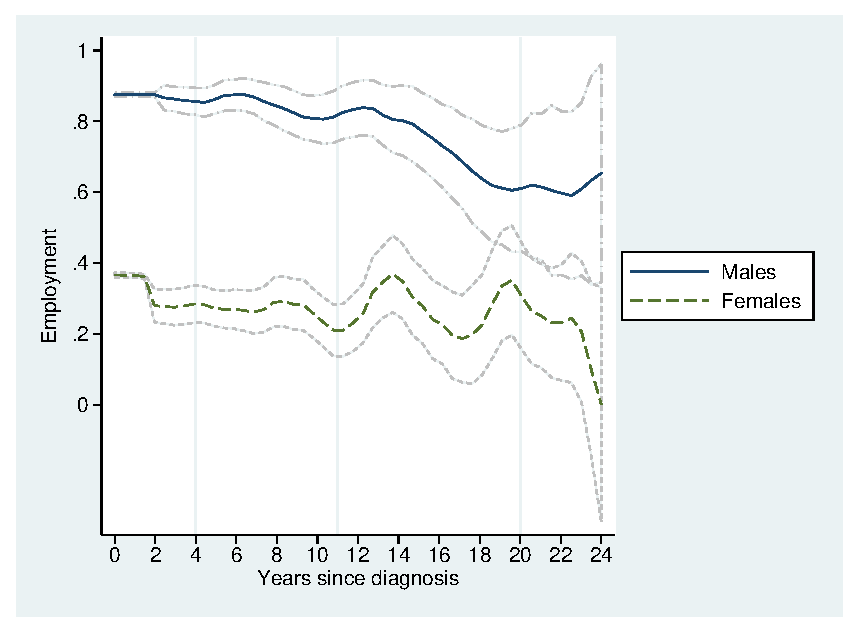
\includegraphics[width=\linewidth]{Chapter4/Figures/lpoly_works_diabetesduration.eps}\\
\footnotesize{\textit{Notes} The dotted lines around the main line show 95\% confidence intervals.}
\end{center}
\end{figure}

\newpage
\begin{figure}[h!]
\caption{\label{fig:Kernel-weighted-local-polynomial_wage}Kernel-weighted local
polynomial regression of log hourly wages on diabetes duration.}%
\begin{center}
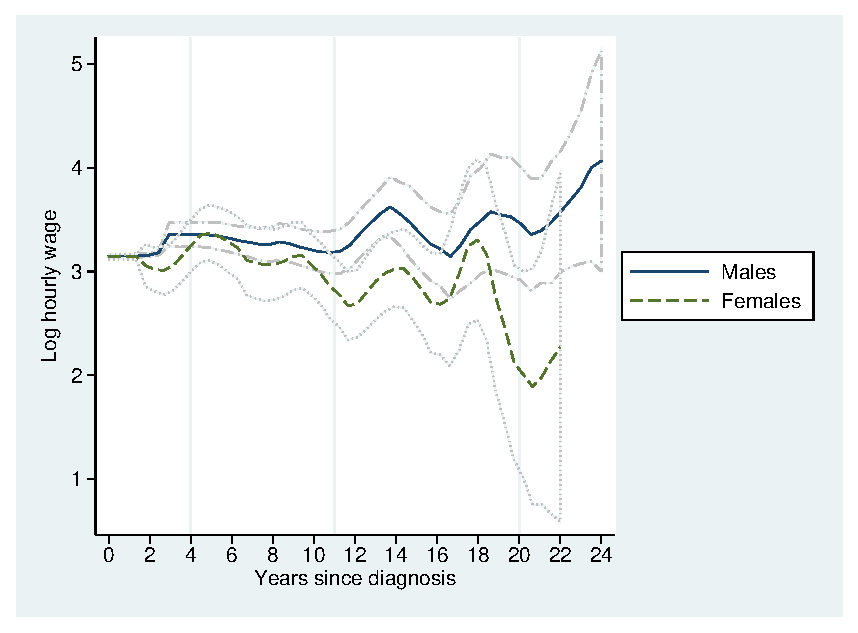
\includegraphics[width=\linewidth]{Chapter4/Figures/lpoly_wage_diabetesduration.eps}\\
\footnotesize{\textit{Notes} The dotted lines around the main line show 95\% confidence intervals.}
\end{center}
\end{figure}

\newpage
\begin{figure}[h!]
\caption{\label{fig:Kernel-weighted-local-polynomial_workhrs}Kernel-weighted local
polynomial regression of working hours on diabetes duration.}%
\begin{center}
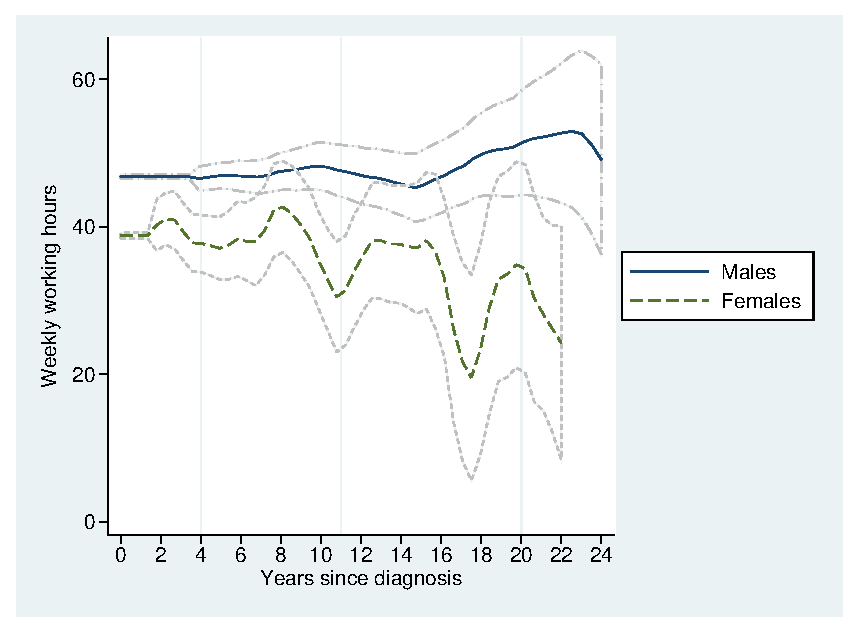
\includegraphics[width=\linewidth]{Chapter4/Figures/lpoly_workhrs_diabetesduration.eps}\\
\footnotesize{\textit{Notes} The dotted lines around the main line show 95\% confidence intervals.}
\end{center}
\end{figure}
\clearpage





\begin{table}[p]
\caption{\label{tab:Self-reported-diabetes-duration_employ}Relationship between self-reported years since diagnosis and employment probabilities using continuous duration and duration splines.}
\begin{center}
%\resizebox{\linewidth}{!}{%
\begin{adjustbox}{max width=\linewidth}
\begin{threeparttable}

{
\def\sym#1{\ifmmode^{#1}\else\(^{#1}\)\fi}
\begin{tabular}{l*{6}{S
S}}
\toprule
                &\multicolumn{3}{c}{Males}                               &\multicolumn{3}{c}{Females}                             \\\cmidrule(lr){2-4}\cmidrule(lr){5-7}
                &\multicolumn{1}{c}{(1)}&\multicolumn{1}{c}{(2)}&\multicolumn{1}{c}{(3)}&\multicolumn{1}{c}{(4)}&\multicolumn{1}{c}{(5)}&\multicolumn{1}{c}{(6)}\\
                  &\multicolumn{1}{c}{OLS}&\multicolumn{1}{c}{OLS}&\multicolumn{1}{c}{FE}&\multicolumn{1}{c}{OLS}&\multicolumn{1}{c}{OLS}&\multicolumn{1}{c}{FE}\\
                                &\multicolumn{1}{c}{(Wave 3)}&\multicolumn{1}{c}{(Pooled)}&\multicolumn{1}{c}{}&\multicolumn{1}{c}{(Wave 3)}&\multicolumn{1}{c}{(Pooled)}&\multicolumn{1}{c}{}\\
\midrule
\addlinespace
Panel A: linear &&&&&&\\
Diabetes duration &   -.008\sym{***}&    -.007\sym{***}&    -.017\sym{***}&    -.005\sym{***}&    -.004\sym{***}&    -.009\sym{*}  \\
                &   (.002)         &   (.002)         &   (.006)         &   (.002)         &   (.001)         &   (.005)         \\
                
\midrule
                Hausman test    &                  &                  &  153.024         &                  &                  &  200.073         \\
                \hspace*{10mm} p-value         &                  &                  &     .000         &                  &                  &     .000         \\
\midrule
\addlinespace
Panel B: splines&&&&&&\\
Diabetes duration &&&&&&\\
\hspace*{10mm}0--4&    -.007         &    -.007         &    -.026\sym{*}  &    -.010         &    -.015\sym{**} &    -.017         \\
                &   (.007)         &   (.006)         &   (.014)         &   (.007)         &   (.006)         &   (.016)         \\
\hspace*{10mm}5--11&     .000         &    -.003         &    -.003         &    -.004         &     .004         &    -.003         \\
                &   (.009)         &   (.006)         &   (.009)         &   (.008)         &   (.006)         &   (.008)         \\
\hspace*{10mm}12--20&  -.030\sym{**} &    -.017\sym{*}  &    -.029\sym{*}  &     .005         &    -.004         &    -.014         \\
                &   (.012)         &   (.010)         &   (.016)         &   (.008)         &   (.006)         &   (.011)         \\
\hspace*{10mm}> 20&     .011         &     .007         &    -.046\sym{*}  &    -.010\sym{*}  &    -.003         &    -.015         \\
                &   (.016)         &   (.014)         &   (.028)         &   (.006)         &   (.003)         &   (.018)         \\
\midrule
Hausman test    &                  &                  &  161.953         &                  &                  &  198.692         \\
\hspace*{10mm} p-value         &                  &                  &     .000         &                  &                  &     .000         \\
N               &     8217         &    16292         &    16292         &    10467         &    22407         &    22407         \\
\bottomrule
\end{tabular}
\begin{tablenotes}
\item \footnotesize \textit{Notes} The table presents the results of three estimation methods. Panel A presents the results of the linear specifications. Panel B presents the results of the non-linear specifications. Robust standard errors in parentheses. Other control variables: state dummies, urbanization dummies, education dummies, married dummy, number children < 6, wealth, age squared and calendar year dummies. The OLS and pooled OLS models additionally control for age. \sym{*} \(p<0.10\), \sym{**} \(p<0.05\), \sym{***} \(p<0.01\).
\end{tablenotes}
}
\end{threeparttable}
\end{adjustbox}
\end{center}
\end{table}


\begin{table}[p]
\caption{\label{tab:Self-reported-diabetes-duration_wage}Relationship between self-reported years since diagnosis and log hourly wage / weekly working hours using continuous duration and duration splines.}
\begin{center}
%\resizebox{\linewidth}{!}{%
\begin{adjustbox}{max width=\linewidth}
\begin{threeparttable}

{
\def\sym#1{\ifmmode^{#1}\else\(^{#1}\)\fi}
\begin{tabular}{l*{6}{S
S}}
\toprule
                &\multicolumn{3}{c}{Males}                               &\multicolumn{3}{c}{Females}                             \\\cmidrule(lr){2-4}\cmidrule(lr){5-7}
                &\multicolumn{1}{c}{(1)}&\multicolumn{1}{c}{(2)}&\multicolumn{1}{c}{(3)}&\multicolumn{1}{c}{(4)}&\multicolumn{1}{c}{(5)}&\multicolumn{1}{c}{(6)}\\
                &\multicolumn{1}{c}{OLS}&\multicolumn{1}{c}{OLS}&\multicolumn{1}{c}{FE}&\multicolumn{1}{c}{OLS}&\multicolumn{1}{c}{OLS}&\multicolumn{1}{c}{FE}\\
                 &\multicolumn{1}{c}{(wave 3)}&\multicolumn{1}{c}{(pooled)}&\multicolumn{1}{c}{}&\multicolumn{1}{c}{(wave 3)}&\multicolumn{1}{c}{(pooled)}&\multicolumn{1}{c}{}\\
\midrule

                &\multicolumn{6}{c}{\textbf{Log hourly wages}}\\
                \addlinespace
Panel A: linear &&&&&&\\
Diabetes duration&  .001         &     .010\sym{**} &    -.019         &    -.014\sym{*}  &    -.009         &    -.073\sym{**} \\
                &   (.006)         &   (.005)         &   (.018)         &   (.008)         &   (.008)         &   (.029)         \\
\midrule                
Hausman test    &                  &                  &  838.213         &                  &                  &   93.232         \\
\hspace*{10mm} p-value         &                  &                  &     .000         &                  &                  &     .000         \\                
\midrule
\addlinespace
Panel B: splines&&&&&&\\
Diabetes duration&&&&&&\\
\hspace*{10mm}0--4&      .034\sym{*}  &     .046\sym{***}&     .033         &     .027         &     .030         &     .015         \\
                &   (.017)         &   (.016)         &   (.055)         &   (.031)         &   (.026)         &   (.138)         \\
\hspace*{10mm}5--11&    -.041\sym{*}  &    -.037\sym{**} &    -.055\sym{*}  &    -.039         &    -.034         &    -.101\sym{*}  \\
                &   (.021)         &   (.018)         &   (.033)         &   (.030)         &   (.024)         &   (.056)         \\
\hspace*{10mm}12--20&      0.015         &     .044         &     .062         &    -.032         &    -.071\sym{*}  &    -.051         \\
                &   (.033)         &   (.029)         &   (.056)         &   (.042)         &   (.039)         &   (.047)         \\
\hspace*{10mm}> 20&     .053         &     .014         &    -.111         &    -.007         &     .041\sym{***}&    -.204\sym{***}\\
                &   (.054)         &   (.040)         &   (.104)         &   (.028)         &   (.015)         &   (.053)         \\
\midrule
Hausman test    &                  &                  & 1037.290         &                  &                  &   96.266         \\
\hspace*{10mm} p-value         &                  &                  &     .000         &                  &                  &     .000         \\
N               &     5509         &    10767         &    10767         &     2874         &     5741         &     5741         \\
\bottomrule
\addlinespace
&\multicolumn{6}{c}{\textbf{Weekly working hours}}\\
\addlinespace
Panel A: linear &&&&&&\\
Diabetes duration & .069         &     .048         &     .181         &    -.020         &    -.124         &     .208         \\
                &   (.124)         &   (.102)         &   (.330)         &   (.187)         &   (.127)         &   (.652)         \\
\midrule
Hausman test    &                  &                  &  704.904         &                  &                  &  107.709         \\
\hspace*{10mm} p-value         &                  &                  &     .000         &                  &                  &     .000         \\
\midrule
\addlinespace
Panel B: splines &&&&&&\\
Diabetes duration &&&&&&\\
\hspace*{10mm}0--4&      -.033         &    -.233         &     .709         &     .739         &     .470         &    2.014         \\
                &   (.421)         &   (.325)         &   (.938)         &   (.645)         &   (.586)         &  (2.947)         \\
\hspace*{10mm}5--11&  .269         &     .338         &    -.218         &    -.410         &    -.479         &    -.508         \\
                &   (.539)         &   (.399)         &   (.568)         &   (.728)         &   (.553)         &  (1.020)         \\
\hspace*{10mm}12--20&    .209         &     .137         &     .698         &    -.164         &    -.051         &    -.402         \\
                &   (.730)         &   (.538)         &   (.945)         &   (.995)         &   (.700)         &  (1.207)         \\
\hspace*{10mm}> 20&  -1.300         &    -.768         &     .039         &    -.499         &    -.418         &    8.117\sym{***}\\
                &   (.944)         &   (.930)         &  (2.184)         &   (.930)         &   (.305)         &  (1.612)         \\
\midrule
Hausman test    &                  &                  &  724.225         &                  &                  &  112.627         \\
\hspace*{10mm} p-value         &                  &                  &     .000         &                  &                  &     .000         \\
N               &     6807         &    13581         &    13581         &     3591         &     7383         &     7383         \\
\bottomrule
\end{tabular}
\begin{tablenotes}
\item \footnotesize \textit{Notes} The table presents the results of three estimation methods for the two dependent variables: log hourly wages and weekly working hours. Panel A presents the results of the linear specifications. Panel B presents the results of the non-linear specifications. Robust standard errors in parentheses. Other control variables: state dummies, urbanization dummies, education dummies, married dummy, number children < 6, wealth, age squared, calendar year dummies, type of work (agricultural and self employed with dependent non-agricultural wage employment as the base) and health insurance status. The OLS and pooled OLS models additionally control for age. \sym{*} \(p<0.10\), \sym{**} \(p<0.05\), \sym{***} \(p<0.01\).
\end{tablenotes}
}
\end{threeparttable}
\end{adjustbox}
\end{center}
\end{table}

%\FloatBarrier

\subsection{Cross-sectional biomarker analysis}


In this section we gain additional insights from using the biomarker data collected in the
third wave of the \ac{MxFLS}. These data enable us to identify respondents with
\ac{HbA1c} levels equal to or above the internationally recognized diabetes threshold of 6.5\%. This will allow the investigation of the direction of bias introduced when relying on self-reported diabetes only and when it is not possible to identify those unaware as well.

We first present a cross tabulation of self-reported diabetes and the results of the biomarker analysis (Table  \ref{tab:Biomarker_observations}). The table shows that 27\% of the sample have \ac{HbA1c} levels indicative of diabetes and 81\% of those self-reporting a diabetes diagnosis also have \ac{HbA1c} levels equal to or above the diabetes threshold. Overall, of the people with diabetes according to the biomarker analysis, 32\% self-report a diagnosis, while 68\% do not.


\begin{table}[p]
\caption{\label{tab:Biomarker_observations}Number of observations with diabetes (HbA1c $\geq 6.5\%$) and self-reported diabetes.}
\begin{center}
\begin{adjustbox}{max width=\linewidth}
\begin{threeparttable}
{
\def\sym#1{\ifmmode^{#1}\else\(^{#1}\)\fi}
\begin{tabular}{l*{3}{S S}}
\toprule
            &\multicolumn{1}{c}{$HbA1c < 6.5\%$}&\multicolumn{1}{c}{HbA1c $\geq 6.5\%$}&\multicolumn{1}{c}{Total}\\
\midrule
No self-reported diabetes & 4544 & 1181 & 5725 &  \\
 & 79\% & 21\% & 100\% &  \\
& 97\% & 68\% & 89\% &  \\
Self-reported diabetes & 129 & 554 & 683 &  \\
 & 19\% & 81\% & 100\% &  \\
 & 3\% & 32\% & 11\% &  \\
Total & 4673 & 1735 & 6408 &  \\
 & 73\% & 27\% & 100\% &  \\
  & 100\% & 100\% & 100\% &  \\
\bottomrule
\end{tabular}
\begin{tablenotes}
\item \footnotesize \textit{Notes} The first row of each category presents absolute values, the second row presents row percentages and the third row present column percentages.
\end{tablenotes}
}
\end{threeparttable}
\end{adjustbox}
\end{center}
\end{table}

To further investigate the relationship of self-reported and biomarker tested diabetes, we estimate the models presented in equations \ref{eq:diab_sr}, \ref{eq:diab} and \ref{eq:diab_ud}.  
The results in columns 1 and 2 of Table \ref{tab:Biomarker_results} show that the earlier longitudinal results using self-reported diabetes are robust for the biomarker sample. The coefficients in column 3 and 4 indicate that the associations with employment probabilities are much weaker when using diabetes defined by the biomarker instead of self-reported diabetes.\footnote{We also created a dummy variable that additionally to measured diabetes accounted for those with a self-reported diabetes diagnosis but biomarker levels below the diabetes threshold. This allowed us to investigate the effect for the entire diabetes population. The coefficients and their statistical significance are only marginally different to those presented in columns 3 and 4 of Table \ref{tab:Biomarker_results}, which is why we do not present them here.} In columns 5 and 6, obtained from estimating Eq. \ref{eq:diab_ud}, the coefficient for the biomarker diabetes population $Dbio_i$ now reflects the effect of undiagnosed diabetes, as the regression includes a control for self-reported diabetes, revealing that undiagnosed diabetes is not associated with any of the labour market outcomes. 

\newpage
\begin{table}[p]
\caption{\label{tab:Biomarker_results}Biomarker results}
\begin{center}
\begin{adjustbox}{max width=\linewidth}
\begin{threeparttable}
{
\def\sym#1{\ifmmode^{#1}\else\(^{#1}\)\fi}
\begin{tabular}{l*{6}{S
S}}
\toprule
                &\multicolumn{2}{c}{Self-reported diabetes}    &\multicolumn{2}{c}{HbA1c $\geq$ 6.5}&\multicolumn{2}{c}{HbA1c $\geq$ 6.5 and self-reported d.}                 \\\cmidrule(lr){2-3}\cmidrule(lr){4-5}\cmidrule(lr){6-7}
                &\multicolumn{1}{c}{(1)}&\multicolumn{1}{c}{(2)}&\multicolumn{1}{c}{(3)}&\multicolumn{1}{c}{(4)}&\multicolumn{1}{c}{(5)}&\multicolumn{1}{c}{(6)}\\
                &\multicolumn{1}{c}{Males}&\multicolumn{1}{c}{Females}&\multicolumn{1}{c}{Males}&\multicolumn{1}{c}{Females}&\multicolumn{1}{c}{Males}&\multicolumn{1}{c}{Females}\\
\midrule
\multicolumn{7}{l}{\hspace*{10mm}\textbf{Dependent variable: Employment}} \\
Self-reported diabetes&   -.051\sym{**} &    -.044\sym{*}  &                  &                  &    -.053\sym{**} &    -.032         \\
                &   (.026)         &   (.023)         &                  &                  &   (.026)         &   (.026)         \\
HbA1c $\geq$ 6.5&                  &                  &    -.012         &    -.031\sym{*}  &     .003         &    -.022         \\
                &                  &                  &   (.016)         &   (.018)         &   (.017)         &   (.019)         \\
\midrule
N               &\multicolumn{1}{S}{2785}         &\multicolumn{1}{S}{3623}         &\multicolumn{1}{S}{2785}         &\multicolumn{1}{S}{3623}         &\multicolumn{1}{S}{2785}         &\multicolumn{1}{S}{3623}         \\
\midrule
\multicolumn{7}{l}{\hspace*{10mm}\textbf{Dependent variable: Log hourly wages}} \\ 
\addlinespace
Self-reported diabetes&    -.010         &    -.040         &                  &                  &    -.006         &    -.010         \\
                &   (.065)         &   (.113)         &                  &                  &   (.078)         &   (.119)         \\
HbA1c $\geq$ 6.5&                  &                  &    -.007         &    -.057         &    -.006         &    -.055         \\
                &                  &                  &   (.044)         &   (.070)         &   (.049)         &   (.075)         \\
\midrule
N               &\multicolumn{1}{S}{1803}         &\multicolumn{1}{S}{884}         &\multicolumn{1}{S}{1803}         &\multicolumn{1}{S}{884}         &\multicolumn{1}{S}{1803}         &\multicolumn{1}{S}{884}         \\
\midrule
\multicolumn{7}{l}{\hspace*{10mm}\textbf{Dependent variable: Weekly working hours}} \\ 
\addlinespace
Self-reported diabetes&   -.293         &    -.751         &                  &                  &    -.286         &   -1.566         \\
                &  (1.305)         &  (2.178)         &                  &                  &  (1.419)         &  (2.351)         \\
HbA1c $\geq$ 6.5&                  &                  &    -.088         &    1.153         &    -.012         &    1.525         \\
                &                  &                  &   (.844)         &  (1.462)         &   (.925)         &  (1.565)         \\
\bottomrule
\end{tabular}
\begin{tablenotes}
\item \footnotesize \textit{Notes} Community level fixed effects. Robust standard errors in parentheses. Other control variables: age, age squared, state dummies, urbanization dummies, education dummies, married dummy, number children < 6 and wealth. Calender year dummies are included as data collection for the third wave was stretched out over several years. The wage and working hour models additionally control for type of work (agricultural and self employed with non-agricultural wage employment as the base) and for health insurance status. \sym{*} \(p<0.10\), \sym{**} \(p<0.05\), \sym{***} \(p<0.01\).
\end{tablenotes}
}
\end{threeparttable}
\end{adjustbox}
\end{center}
\end{table}


As discussed earlier, differences in effects between self-reported diabetes and those undiagnosed are likely to stem from selection into the diagnosed population, for instance those in worse health, with higher \ac{HbA1c} levels or a longer disease duration are more likely to go to the doctor and be diagnosed as well as to lose their job because of their diabetes. To further explore this, we first estimate models additionally controlling for self-reported health status to capture differences in subjective individual health. Secondly, we estimate models accounting for measured \ac{HbA1c} levels, to  investigate in how far current diabetes severity affects our labour market outcomes. If current severity would be related to labour market outcomes and explain the difference between self-reported and the undiagnosed diabetes population, one would expect an adverse association with increasing \ac{HbA1c} levels, for both self-reporting and undiagnosed. To investigate this, we construct three dummy variables using \ac{HbA1c} groups above the diabetes threshold (i.e. 6.5--7.9, 8--11.9 and 12--14), each for those with self-reported diabetes and for those unaware of their diabetes (Table \ref{tab:Diagnosed_undiagnosed_robust}, Panel B).

\begin{table}[p]
\caption{\label{tab:Diagnosed_undiagnosed_robust}Self-reported diabetes, biomarkers, diabetes severity and self-reported health and their association with labour market outcomes}
\begin{center}
\begin{adjustbox}{max width=\linewidth} 
\begin{threeparttable} 
{
\def\sym#1{\ifmmode^{#1}\else\(^{#1}\)\fi}
\begin{tabular}{l*{6}{S
S}}
\toprule
                &\multicolumn{2}{c}{Employment}       &\multicolumn{2}{c}{Log hourly wages} &\multicolumn{2}{c}{Weekly working hours}\\\cmidrule(lr){2-3}\cmidrule(lr){4-5}\cmidrule(lr){6-7}
                &\multicolumn{1}{c}{(1)}&\multicolumn{1}{c}{(2)}&\multicolumn{1}{c}{(3)}&\multicolumn{1}{c}{(4)}&\multicolumn{1}{c}{(5)}&\multicolumn{1}{c}{(6)}\\
                &\multicolumn{1}{c}{Males}&\multicolumn{1}{c}{Females}&\multicolumn{1}{c}{Males}&\multicolumn{1}{c}{Females}&\multicolumn{1}{c}{Males}&\multicolumn{1}{c}{Females}\\
\midrule
\multicolumn{6}{l}{\hspace*{10mm}\textbf{Panel A (self-reported health)}}\\  
Self-reported diabetes&   -.036         &    -.023         &     .002         &     .060         &     .123         &   -2.191         \\
                &   (.026)         &   (.027)         &   (.079)         &   (.121)         &  (1.433)         &  (2.386)         \\        
HbA1c $\geq 6.5\%$&       .003         &    -.023         &    -.004         &    -.051         &    -.066         &    1.829         \\
                &   (.017)         &   (.019)         &   (.049)         &   (.075)         &   (.926)         &  (1.569)         \\
\multicolumn{6}{l}{Self-reported health status}\\
\hspace*{10mm}good&    .023         &     .057\sym{*}  &     .061         &    -.115         &   -1.131         &    3.521         \\
                &   (.025)         &   (.034)         &   (.074)         &   (.124)         &  (1.376)         &  (2.499)         \\
\hspace*{10mm}fair&    -.007         &     .006         &     .025         &    -.157         &   -1.606         &    4.646\sym{*}  \\
                &   (.026)         &   (.034)         &   (.076)         &   (.128)         &  (1.424)         &  (2.607)         \\
\hspace*{10mm}bad &    -.127\sym{***}&    -.024         &    -.016         &    -.371\sym{*}  &   -6.190\sym{**} &    6.918\sym{*}  \\
                &   (.043)         &   (.046)         &   (.135)         &   (.189)         &  (2.521)         &  (3.858)         \\
\hspace*{10mm}very bad&    -.165         &     .117         &    -.331         &     .316         &   -1.869         &  -17.400\sym{*}  \\
                &   (.110)         &   (.116)         &   (.300)         &   (.439)         &  (6.433)         &  (9.005)         \\
\midrule
N               &\multicolumn{1}{S}{2785}         &\multicolumn{1}{S}{3621}         &\multicolumn{1}{S}{1803}         &\multicolumn{1}{S}{883}         &\multicolumn{1}{S}{2302}         &\multicolumn{1}{S}{1143}         \\
\midrule
\multicolumn{6}{l}{\hspace*{10mm}\textbf{Panel B (HbA1c levels)}}\\
\multicolumn{6}{l}{Self-reported diabetes}\\
\hspace*{10mm}$6.5 - 7.9$&    -.126\sym{**} &    -.040         &    -.228\sym{*}  &     .041         &    1.218         &   -9.170\sym{*}  \\
                &   (.059)         &   (.051)         &   (.127)         &   (.269)         &  (2.921)         &  (4.864)         \\
\hspace*{10mm}$8 - 11.9$&    -.052         &    -.051         &     .026         &     .225         &   -1.332         &   -1.086         \\
                &   (.051)         &   (.042)         &   (.107)         &   (.206)         &  (2.298)         &  (4.395)         \\
\hspace*{10mm}12+  &     .011         &     .021         &    -.106         &    -.427         &    1.979         &   -2.518         \\
                &   (.062)         &   (.069)         &   (.156)         &   (.279)         &  (3.692)         &  (5.335)         \\
\multicolumn{6}{l}{Undiagnosed diabetes}\\
\hspace*{10mm}$6.5 - 7.9$&     .005         &    -.002         &     .015         &    -.040         &    1.003         &    3.616         \\
                &   (.022)         &   (.025)         &   (.058)         &   (.099)         &  (1.178)         &  (2.323)         \\
\hspace*{10mm}$8 - 11.9$&     .006         &    -.027         &     .014         &    -.204         &   -1.004         &    -.077         \\
                &   (.035)         &   (.031)         &   (.078)         &   (.129)         &  (1.485)         &  (2.614)         \\
\hspace*{10mm}12+&     .015         &    -.055         &    -.019         &     .169         &   -1.581         &    1.753         \\
                &   (.040)         &   (.046)         &   (.087)         &   (.181)         &  (2.099)         &  (3.978)         \\
\midrule
N               &\multicolumn{1}{S}{2785}         &\multicolumn{1}{S}{3623}         &\multicolumn{1}{S}{1803}         &\multicolumn{1}{S}{884}         &\multicolumn{1}{S}{2302}         &\multicolumn{1}{S}{1144}         \\
\bottomrule
\end{tabular}
\begin{tablenotes}
\item \footnotesize \textit{Notes} Community level fixed effects. Robust standard errors in parentheses. Other control variables: age, age squared, state dummies, urbanization dummies, education dummies, married dummy, number children < 6 and wealth. Calender year dummies are included as data collection for the third wave was stretched out over several years. The wage and working hour models additionally control for type of work (agricultural and self employed with non-agricultural wage employment as the base) and for health insurance status. \sym{*} \(p<0.10\), \sym{**} \(p<0.05\), \sym{***} \(p<0.01\).
\end{tablenotes}
}
\end{threeparttable}
\end{adjustbox}
\end{center}
\end{table}


When additionally controlling for subjective health status, we find that for men and women the difference between self-reported diabetes and undiagnosed diabetes is reduced due to a smaller coefficient for self-reported diabetes (Table \ref{tab:Diagnosed_undiagnosed_robust}, Panel A). Especially for women, the point estimates for self-reported diabetes and undiagnosed diabetes are now virtually the same size, suggesting that differences could be due to the differences in self-reported health. For men, factors not captured by self-reported health may still play a role. \footnote{Additionally accounting for measures of overweight and obesity, self-reported hypertension, heart disease and depression does not further affect the interpretation of the diabetes coefficient.}

Turning to Panel B, we do not find a consistent relationship of increasing \ac{HbA1c} levels with employment chances, especially for those self-reporting, suggesting that current disease severity may not explain the different employment effects of diabetes for the aware and unaware.

To the best of our knowledge only one study has previously used biomarkers to analyse the relationship with labour market outcomes in a comparable population. \textcite{BrownIII2011} use data for a Mexican American population in a broadly comparable way to this paper, though stopping short of investigating the labour market impact of undiagnosed diabetes. In concordance with our results this study also finds that once diabetes is diagnosed, current management plays a minor role in determining labour market outcomes. This is not surprising given that \ac{HbA1c} levels only provide a picture of blood glucose levels over the last three months. They therefore may not be representative of blood glucose levels in the years before and after the diabetes diagnosis which ultimately determine how soon complications appear and how severe they will be.

\parencite{Minor2015} finds for a general USA population, similar to us, that people with undiagnosed diabetes likely, if at all, experience smaller employment penalties than people self-reporting the disease. He finds, however, much bigger effects then we do when estimating the impact of biometrically measured diabetes instead of distinguishing between the self-reporting and those unaware. This may be explained by the fact that in that study the undiagnosed population made up a much smaller share of the overall diabetes population compared to our study, so that self-reported diabetes was still the predominant factor driving the result.  
%\FloatBarrier


\section{\label{sec:cha_4_conclusion}Conclusion}

Diabetes has become one of the most common chronic diseases in middle- and high-income countries, with the potential to severely impact the health and economic well-being of those directly (and possibly indirectly) affected. Yet there remains only limited 'hard' evidence on the economic consequences, especially for these countries. Moreover, what evidence does exist at best partially tackles the econometric challenges involved. 

This paper improves on existing work by addressing several methodological challenges that arise due to the nature of the disease and types of data available, using rich longitudinal panel data from Mexico, a \ac{MIC} for which the biomarker data used in this paper indicates that diabetes, including undiagnosed diabetes, has reached alarming levels.

Apart from providing unique evidence for a developing country, the paper makes methodological contributions for the estimation of labour market effects of diabetes. By estimating individual fixed effects the analysis provides an improved accounting for the endogeneity of self-reported diabetes, as this allows cancelling out the potential role of unobserved individual traits that may affect both labour market outcomes and propensity to self-report (or suffer from) diabetes. Using further information on the year of diagnosis enables us to investigate the potential heterogeneity in the effect of self-reported diabetes on labour market outcomes over time. Finally, taking advantage of biomarker data to identify the entire diabetes population, i.e. including those with undiagnosed diabetes, allows for an assessment of the potential bias in estimates relying on self-reported diabetes (which is still the most frequent measure in the previous literature).

The first part of our results confirms a considerable gap in employment probabilities for both men and women reporting a diabetes diagnosis, compared to those that do not report the condition. We also find some evidence that diabetes is more likely to reduce the probability of employment in the agricultural and self-employment sector, characterized predominantly by informal arrangements, compared to the rest of the workforce. Those who remain employed do not suffer any wage or labour supply effects, possibly because they are still relatively healthy or are able to resort to a type of work that does not entail their diabetes status limiting their work-related performance. More research will be needed to confirm and further investigate this finding as well as its interpretation. 

Regarding the heterogeneity in the effects of diabetes over time, our results indicate an adverse impact of self-reported diabetes on employment chances, with the impact growing in magnitude especially after the first 10 years post-diagnosis. This is plausible in that as time lived with diabetes evolves, complications associated with diabetes tend to become more frequent and more severe \parencite{Adler2003}. Looking at wages as our labour market outcome, we uncover some adverse effects for females, indicating a sizeable reduction with time since diagnosis. These findings may bode ill for countries where diabetes has started appearing at an increasingly younger age, causing people to live with the disease for larger parts of their productive lifespan, possibly exacerbating the economic effects of reduced employment due to diabetes \parencite{Hu2011,Villalpando2010}.

The second part of our results indicates that only relying on self-reported diabetes can lead to an overestimation of the relationship between diabetes and labour market outcomes. We find that a negative relationship only exists for those with self-reported, but not for those with undiagnosed diabetes. This perhaps surprising, notable difference, is at least mediated by the subjective health status being worse for those self-reporting compared to the undiagnosed. Current disease severity, as proxied by \ac{HbA1c} levels, does not appear to play an important role in this context.

Our findings bear several implications. First, when interpreting labour market impact estimates relying on self-reported diabetes, one cannot assume that the results extend to those with undiagnosed diabetes. However, the strategy of simply merging self-reported and undiagnosed in one diabetes category may not be ideal either, as doing so will fail to account for the heterogeneity between the groups in the amount of health information they possess, the time they have already been exposed to elevated blood glucose levels and consequently their subjective as well as true health status, leading to a potentially important loss of information. If, by contrast, both groups are separately accounted for in the model, thereby acknowledging their inherent differences, this allows us to gain information about the distribution of the economic burden across the two groups. 

In the case of Mexico, given that more than 7\% of the Mexican population have been diagnosed with diabetes, the identified reduction in employment probabilities for those with self-reported diabetes still amounts to a significant overall economic burden being associated with (diagnosed) diabetes.

Our results add further weight to the case for reducing the incidence and progression of diabetes. On top of the well-documented health benefits, it appears there are considerable potential gains to be had in terms of increasing the productive lifespan of people. This is of particular importance in \acp{LMIC}, where parental health shocks, related job loss and increasing health expenditures can have repercussions across the entire household. Other family members, including children, may be forced to increase their labour supply and to reduce non-health expenditures in order to prevent deterioration of the household's economic situation. This can lead to forgone investments into child education, showcasing the potential for adverse long-term effects of health shocks due to diabetes \parencite{Bratti2014}. Moreover, the large proportion of undiagnosed people indicates that diagnosis---at least in Mexico---happens too late or not at all, thereby significantly reducing the possibility to prevent complications via appropriate treatment and self-management, which has repercussions by increasing the risk of severe complications appearing early. Hence, much of the health and economic burden may be prevented by earlier diagnosis and, given the generally limited success in achieving good control in Mexico, better treatment of those already diagnosed with diabetes. Ultimately of course, there will be a need to invest in the prevention of diabetes cases in the first place. Taxation of sugar sweetened beverages may be one promising way forward \parencite{Colchero2016}, though the long-term effects in terms of diabetes prevention remain to be demonstrated.Diabetes has become one of the most common chronic diseases in middle- and high-income countries, with the potential to severely impact the health and economic well-being of those directly (and possibly indirectly) affected. Yet there remains only limited 'hard' evidence on the economic consequences, especially for these countries. Moreover, what evidence does exist at best partially tackles the econometric challenges involved. 








\printbibliography
\end{document}          
